\documentclass[xcolor=pdftex,dvipsnames,table]{beamer}
 
 \usepackage{hyperref}
\usepackage[utf8]{inputenc}
\usepackage[absolute,overlay]{textpos}
%\usetheme{AnnArbor}
\usetheme{Boadilla}
\newcommand{\backupbegin}{
   \newcounter{finalframe}
   \setcounter{finalframe}{\value{framenumber}}
}
\newcommand{\backupend}{
   \setcounter{framenumber}{\value{finalframe}}
}
% Use the colors:
\setbeamercolor{title}{fg=black,bg=lightgray}






\begin{document}
\title{Status of disappearing track search with $E_{T}^{miss}$}
\author{\underline{Viktor Kutzner$^1$}, Sam Bein$^1$, Alex Tews$^1$, Isabell Melzer-Pellmann$^2$, Akshansh Singh$^2$, Seh Wook Lee$^3$, Sang-il Pak$^3$, Sezen Sekmen$^3$, } 
\institute{$^1$Hamburg, $^2$DESY, $^3$Kyungpook}
\date{\today} 
%\logo{\includegraphics[height=2.1cm]{pdfs/1-UHHlogo.png}\vspace{1pt}}

\frame{\titlepage{
\begin{textblock*}{5cm}(1cm,6.5cm) % {block width} (coords)

\includegraphics[width=0.8in]{pdfs/2-UHHlogo.png}
\end{textblock*}
\begin{textblock*}{5cm}(10.1cm,6.5cm) % {block width} (coords)
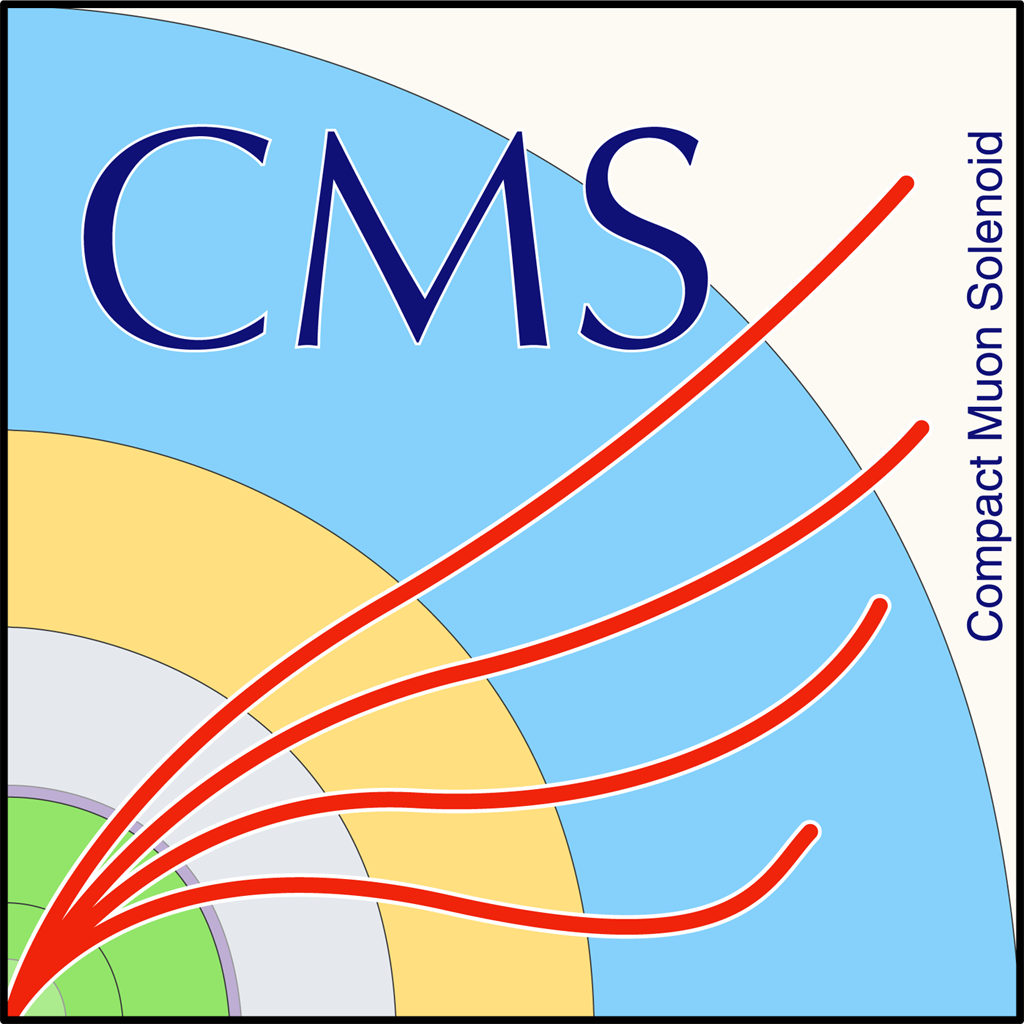
\includegraphics[width=0.8in]{pdfs/3-CMSlogo.png}
\end{textblock*}
}}

\frame{\frametitle{Updates with disappearing tracks with $E_{T}^{miss}$}
\begin{enumerate}
\item Concept refresh 
\begin{itemize}
\item $\rightarrow$selection, search regions, and targeted signal models
\end{itemize}
\item general updates
\begin{itemize}
\item update to track tags with loosened BDTs
\item revisiting fake background closure
\item extend prompt background method to include pions
\item non-pion contamination in $m_{\tau\tau}$
\end{itemize}
\item some changes to the analysis approach seem warranted, so we've made a couple of modifications
\begin{itemize}
\item dropping veto on muons (event-level veto, not object-level)
\item splitting 1-track bins according to high-low track mass observable 
\end{itemize}
\item Signal models and simulation
\begin{itemize}
\item $\rightarrow$ some interesting features seen in the MC
\end{itemize}
\end{enumerate}
\vspace{.5cm}
\scriptsize
Previous updates given in inclusive SUSY meeting \href{https://indico.cern.ch/event/767669/contributions/3188682/attachments/1742622/2820111/susy-status-update-oct26.pdf}{\textbf{link 1}} \href{https://indico.cern.ch/event/767669/contributions/3188682/attachments/1742622/2820111/susy-status-update-oct26.pdf}{\textbf{link 2}}
}

\frame{\frametitle{Key analysis features}
\begin{columns}
\column{.5\textwidth}
\begin{itemize}
\scriptsize
\item Select quality tracks with missing outer hits (DT)
\item Catagorize tracks into short (pixel hits only) and long (pixel and strips hits)
\item Select events with one or more DT's with various topologies
\item Bin search in jet multiplicity to maintain sensitivity to a range of models
\end{itemize}
\centering
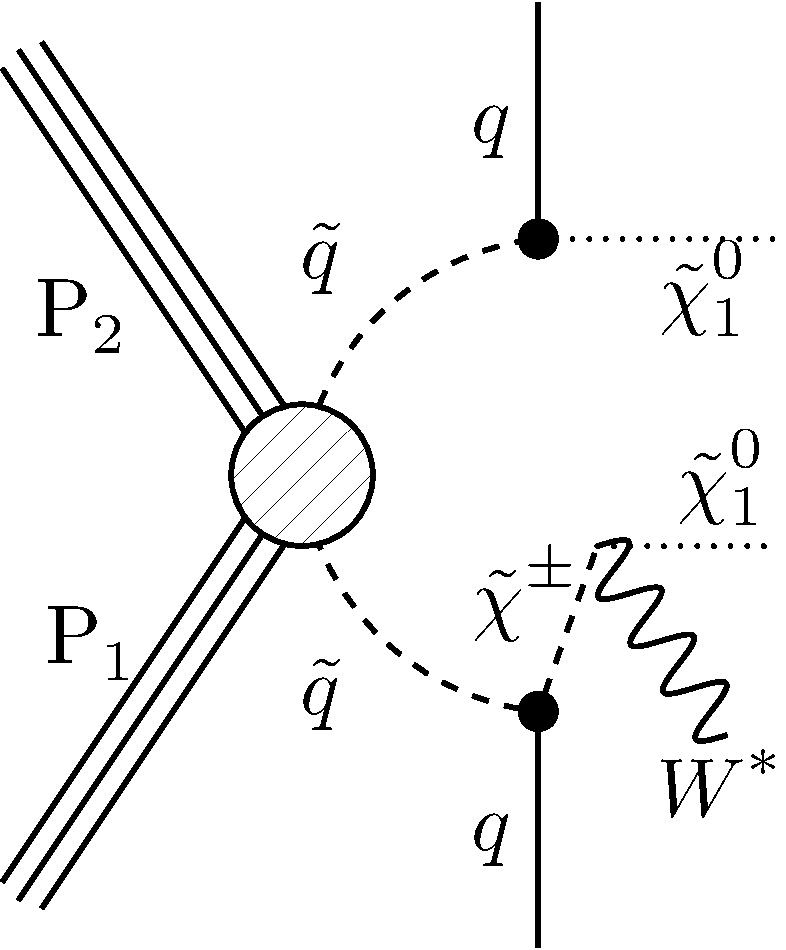
\includegraphics[width=.35\linewidth]{pdfs/4-1b_T3wqq}
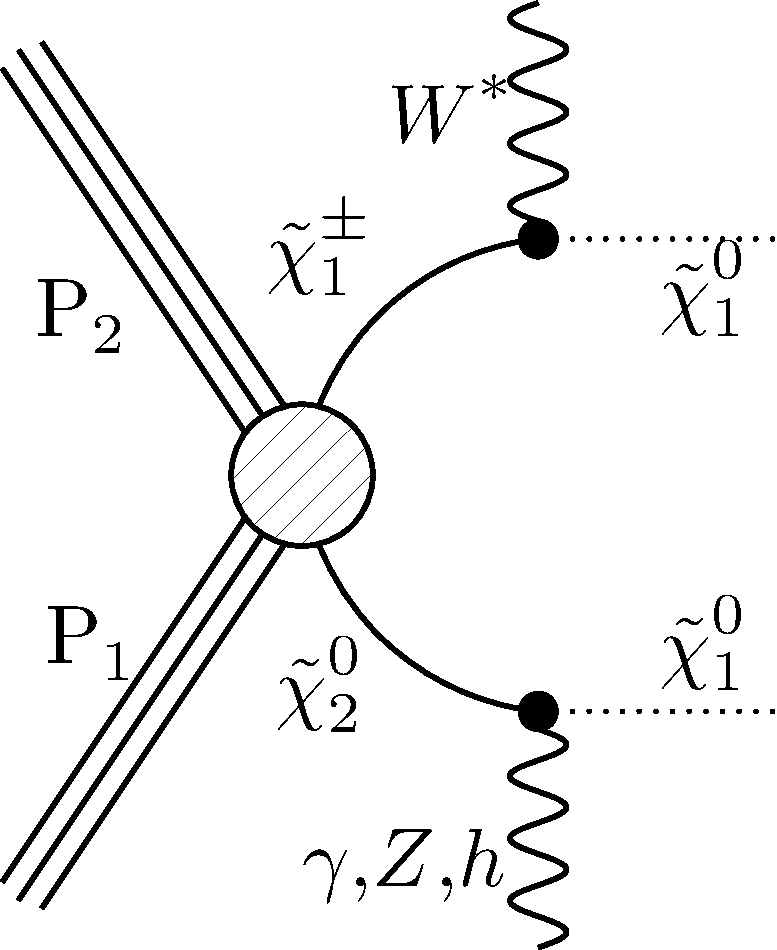
\includegraphics[width=.35\linewidth]{pdfs/5-103b_TChiWB}
\begin{itemize}
\scriptsize
\item Split signal bins into high and low de/dx categories
\end{itemize}
\column{.5\textwidth}
\centering
\scriptsize
Signal regions
\includegraphics[width=.8\linewidth]{pdfs/6-SRTable1}\\
\vspace{-.2cm}
...\\
\vspace{.2cm}
\includegraphics[width=.8\linewidth]{pdfs/7-SRTable3}
\end{columns}
}



\frame{\frametitle{Updated tag}
\centering
\begin{columns}
\column{.5\textwidth}
\begin{itemize}
\scriptsize
\item Before: fully informed BDT (with dxy) 
\item Now: ``uninformed'' BDT without dxy
\item Now: BDT $>60*d_{xy}+0.05$ (long tracks); 
\item analogous cut function for short tracks
\item similar signal efficiency as with informed BDT
\end{itemize}
\centering
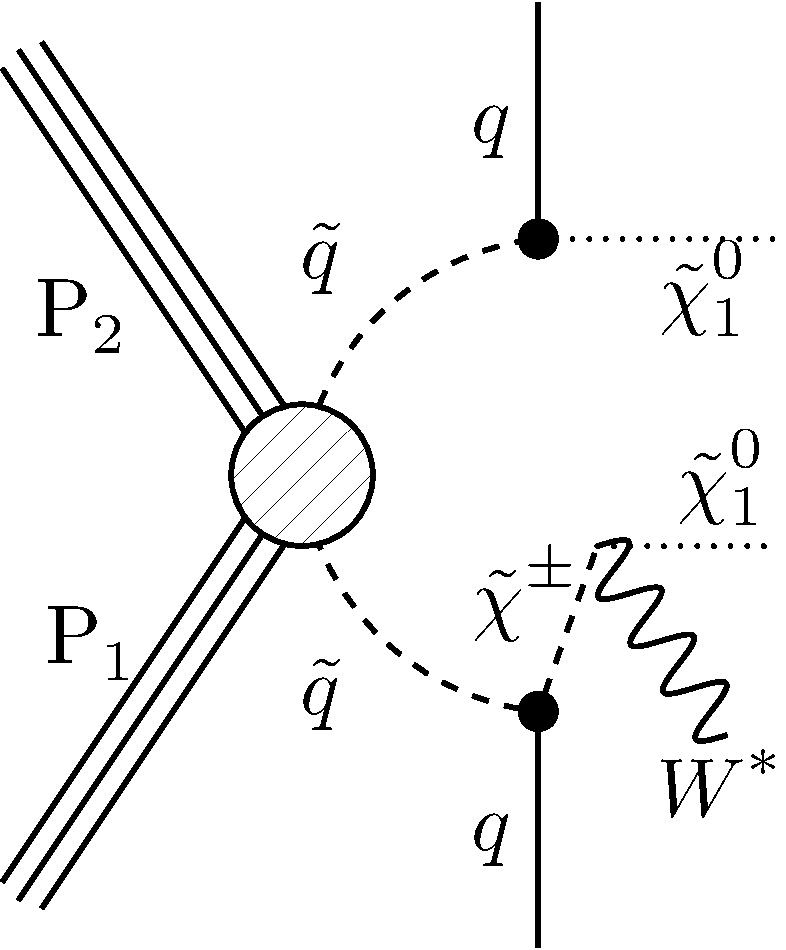
\includegraphics[width=.35\linewidth]{pdfs/8-1b_T3wqq}
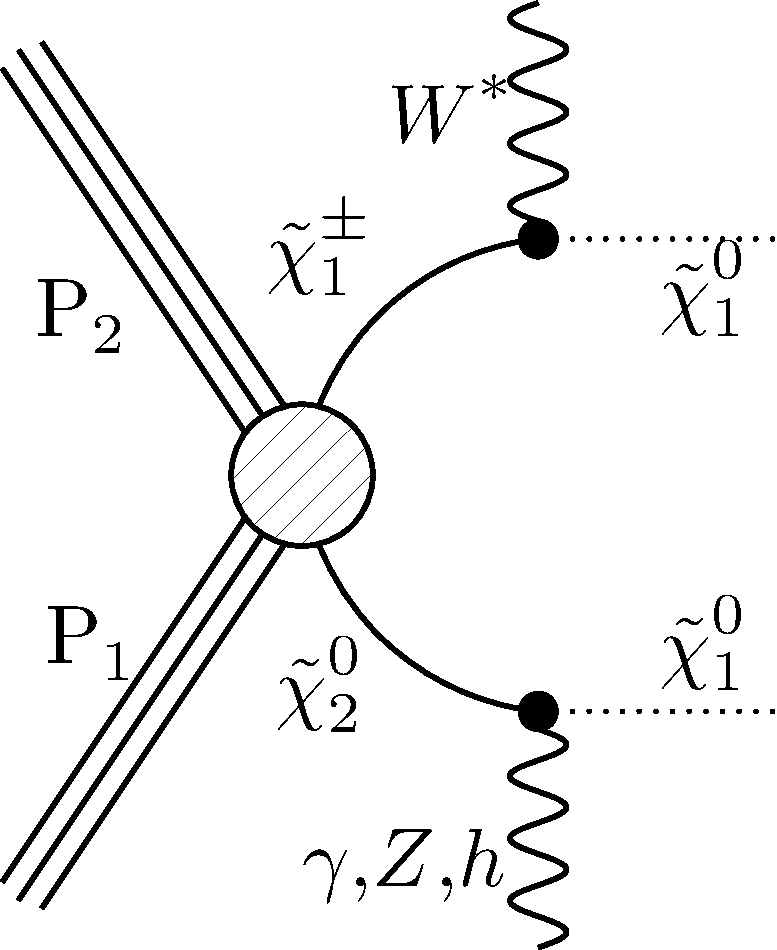
\includegraphics[width=.35\linewidth]{pdfs/9-103b_TChiWB}
\column{.5\textwidth}
\centering
\scriptsize
%plot of uninformed BDT vs dxy (old BDT$>$x)\\
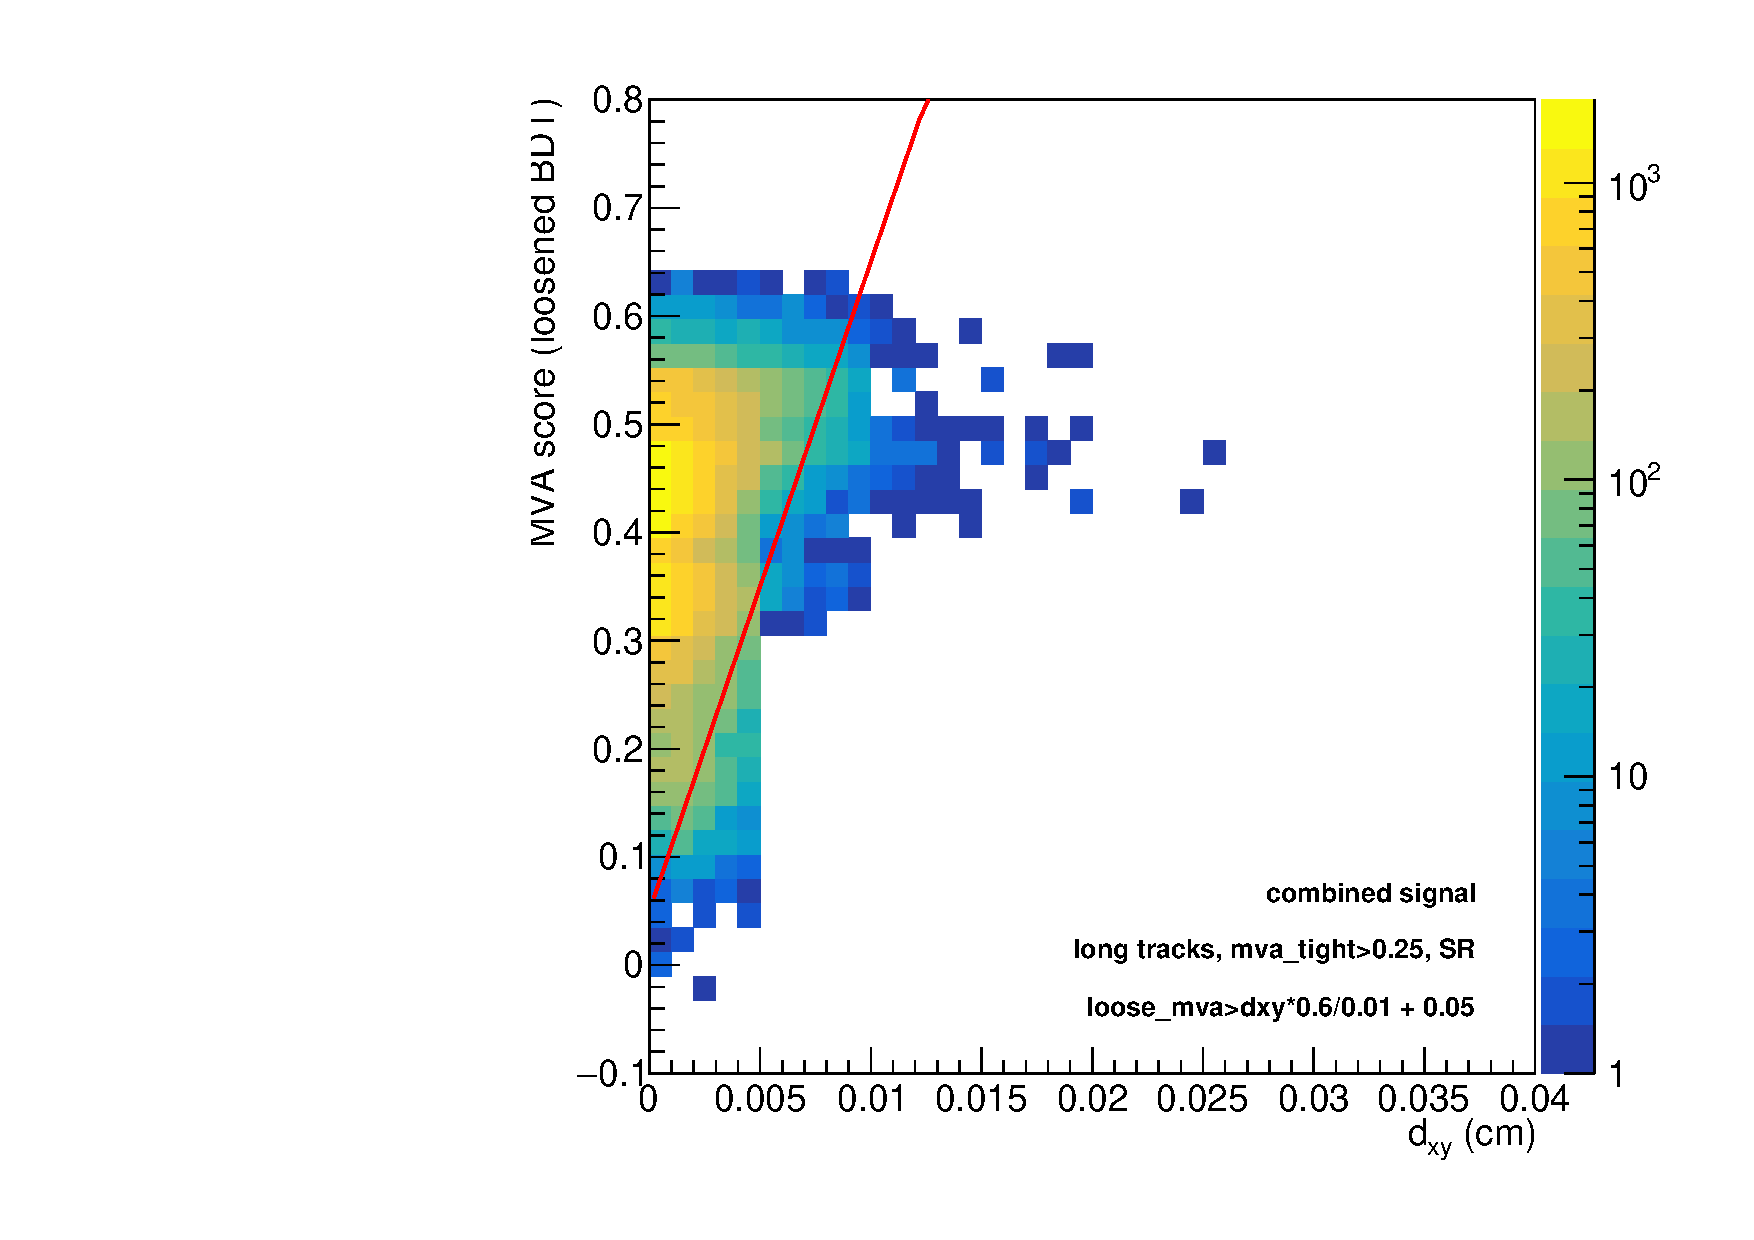
\includegraphics[width=.65\textwidth]{pdfs/2d_long_getfunction_sg.pdf}\\
%plot of uninformed BDT vs dxy (new cut function)
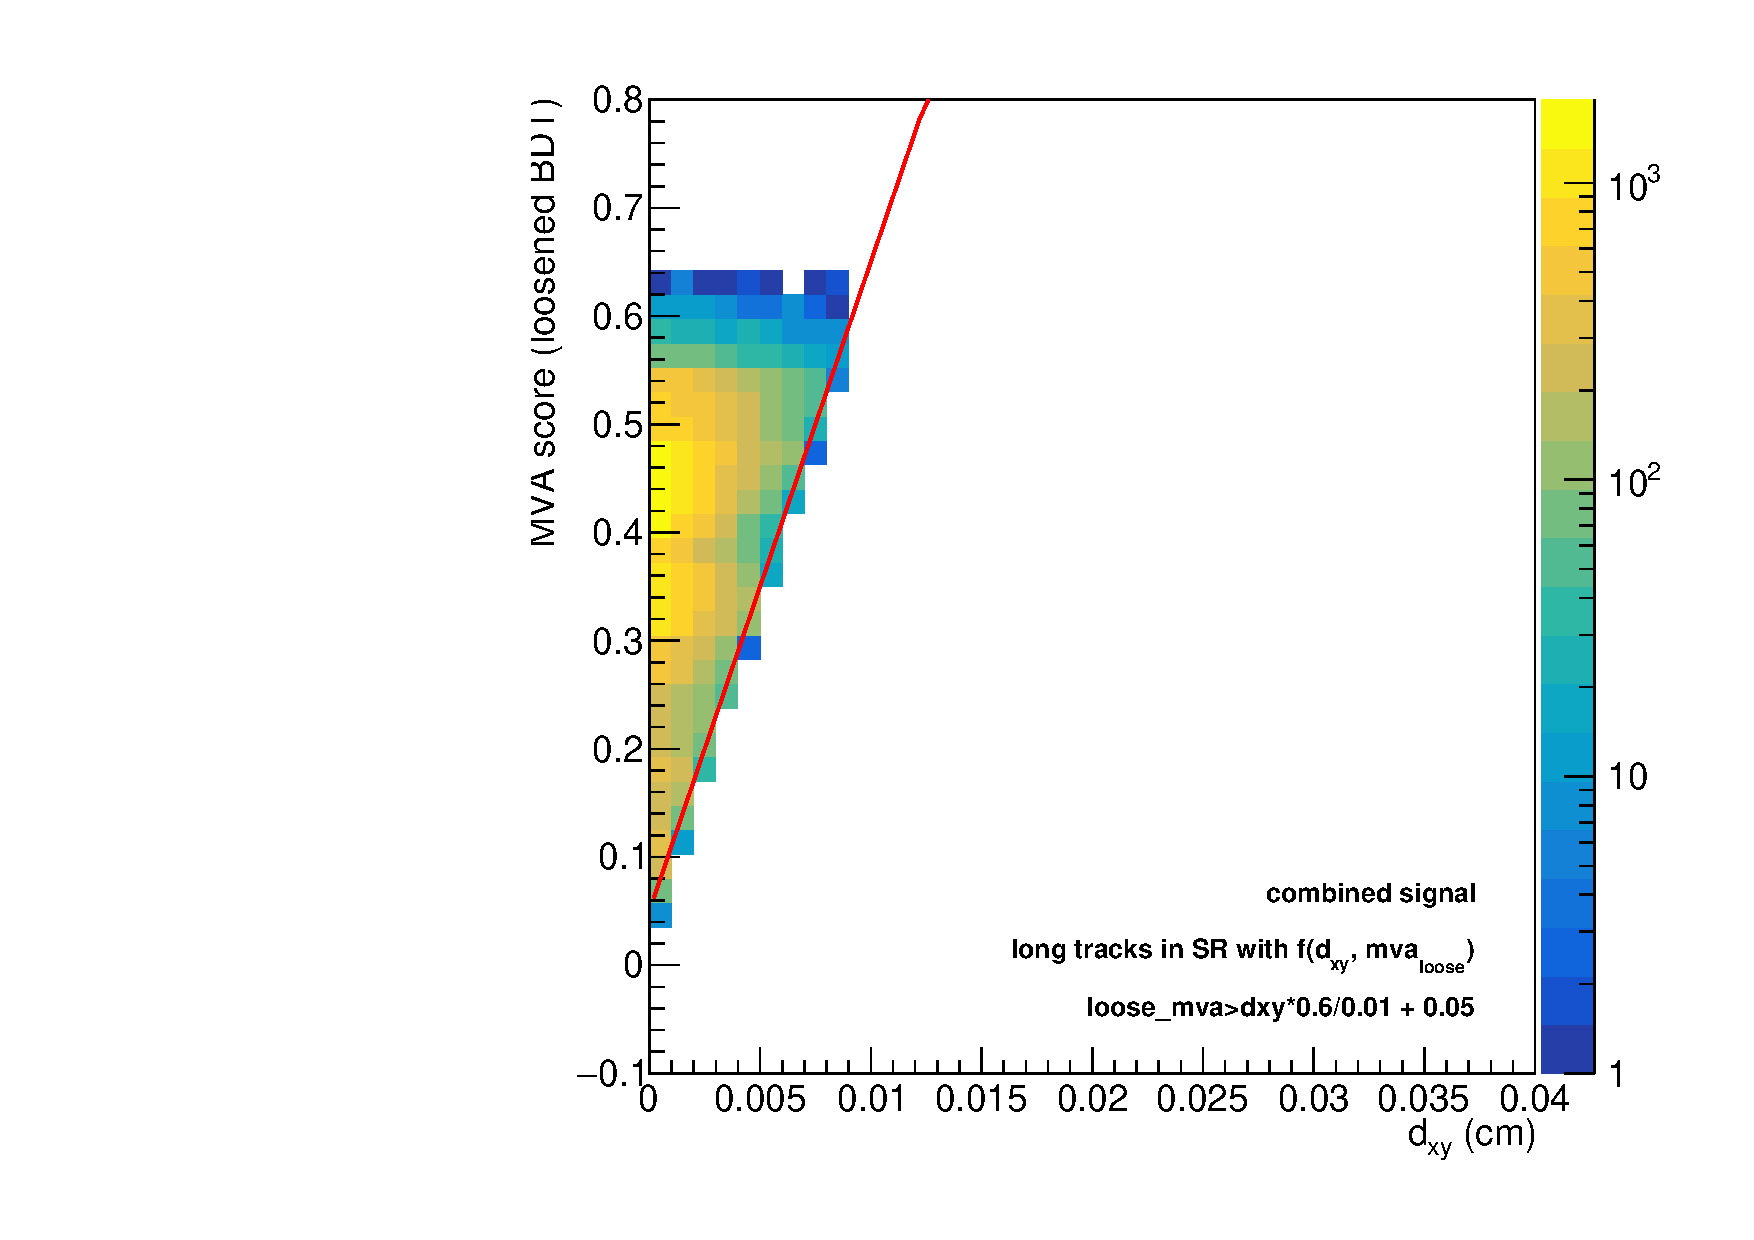
\includegraphics[width=.65\textwidth]{pdfs/2d_long_function_sg.pdf}
\end{columns}
}






\frame{\frametitle{Non-prompt closure}
\centering
\begin{columns}
\column{.5\textwidth}
\begin{itemize}
\scriptsize
\item Use fake rate transfer factor
\end{itemize}
\begin{align*}
\mathcal{F}&= \frac{P(n_{DT}^{SL}=1|\vec{x})}{P(n_{DT}^{CR}=1|\vec{x})}\\
\vec{x} &= {H_{T}, n_{pvtx}}
\end{align*}
\vspace{-.4cm}
\begin{itemize}
\scriptsize
\item SL (signal-like): BDT $>60*d_{xy}+0.05$
\item CR (fake control): BDT $<60*d_{xy}+0.05$
\end{itemize}
\centering
figure of 2-d map
\column{.5\textwidth}
\centering
\scriptsize
%data/MC comparison in CR\\
%closure plot vs NJets or MHT
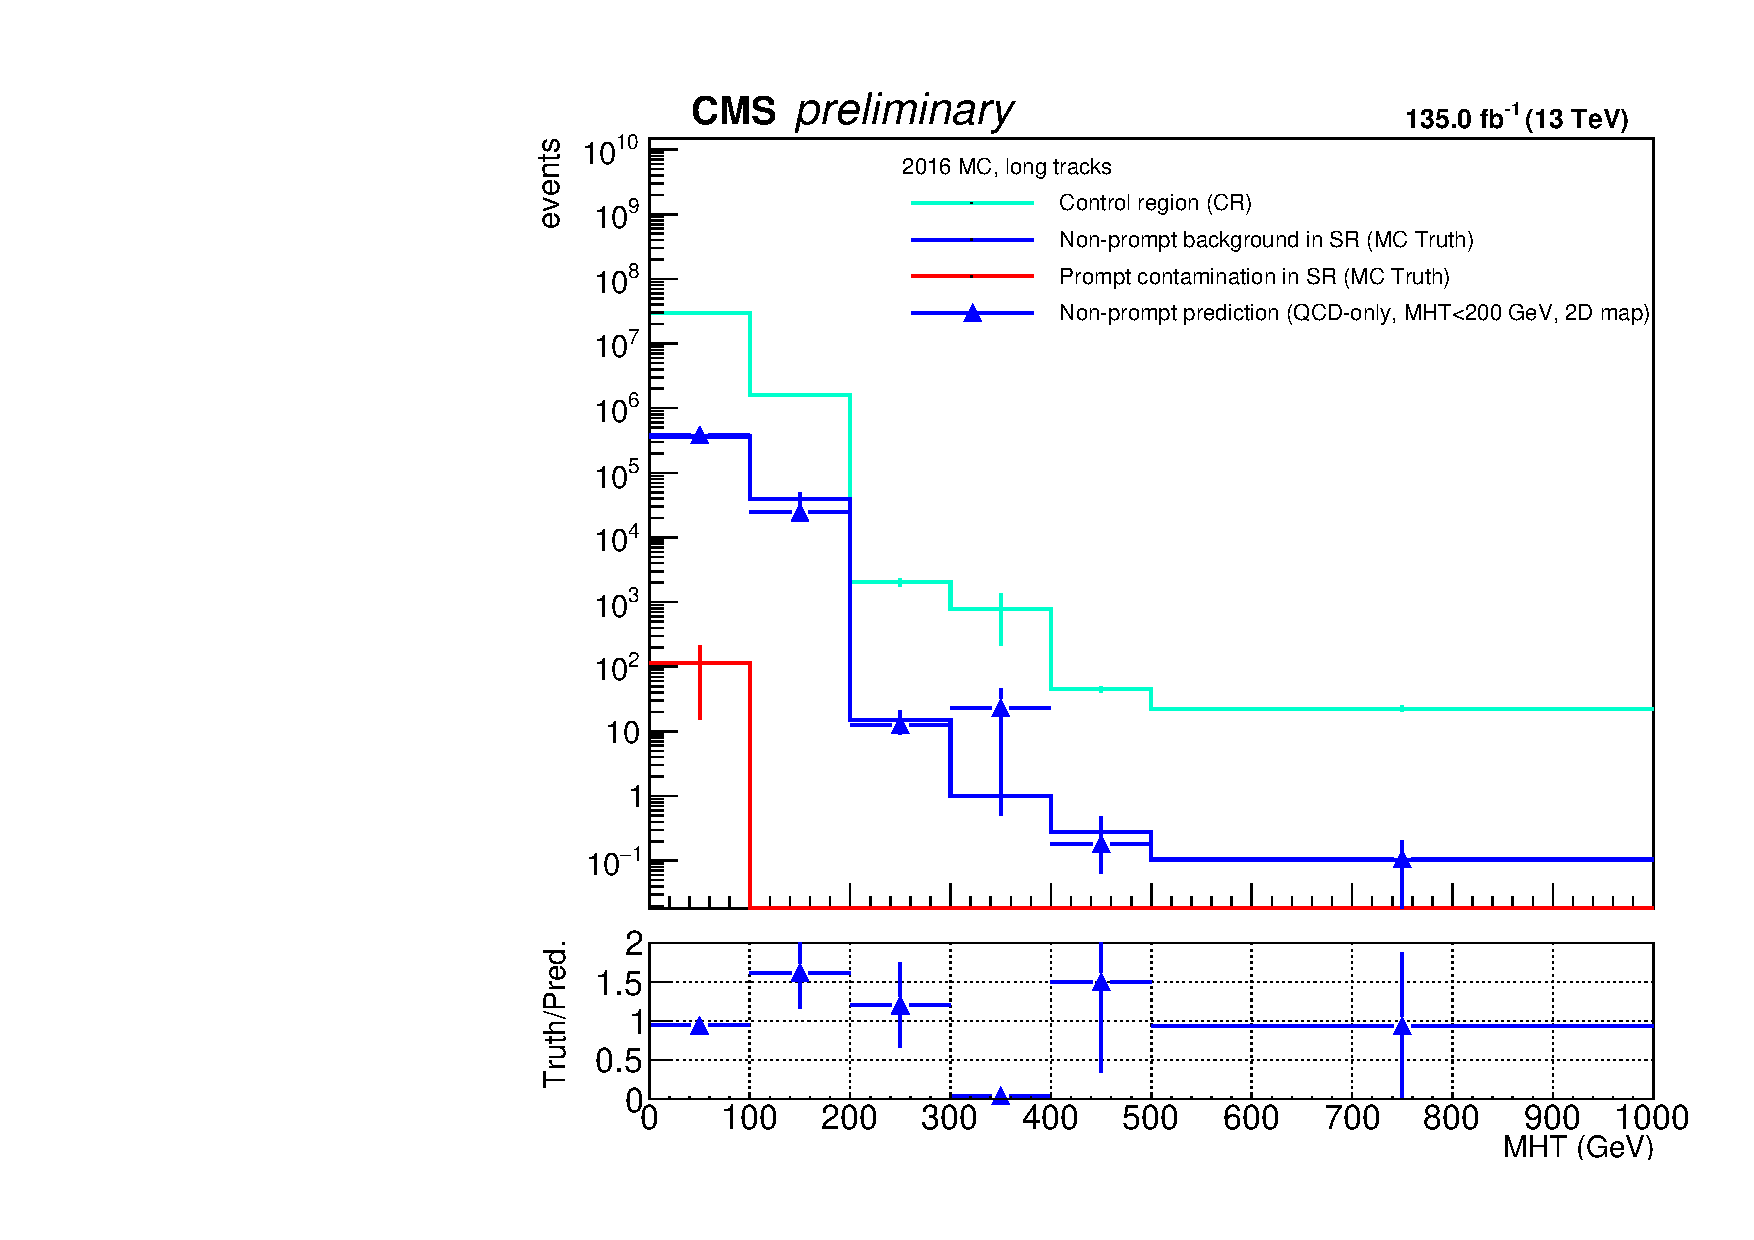
\includegraphics[width=.65\textwidth]{pdfs/prediction_Summer16_MHT_loose5_long_comparison_cr1.pdf}\\
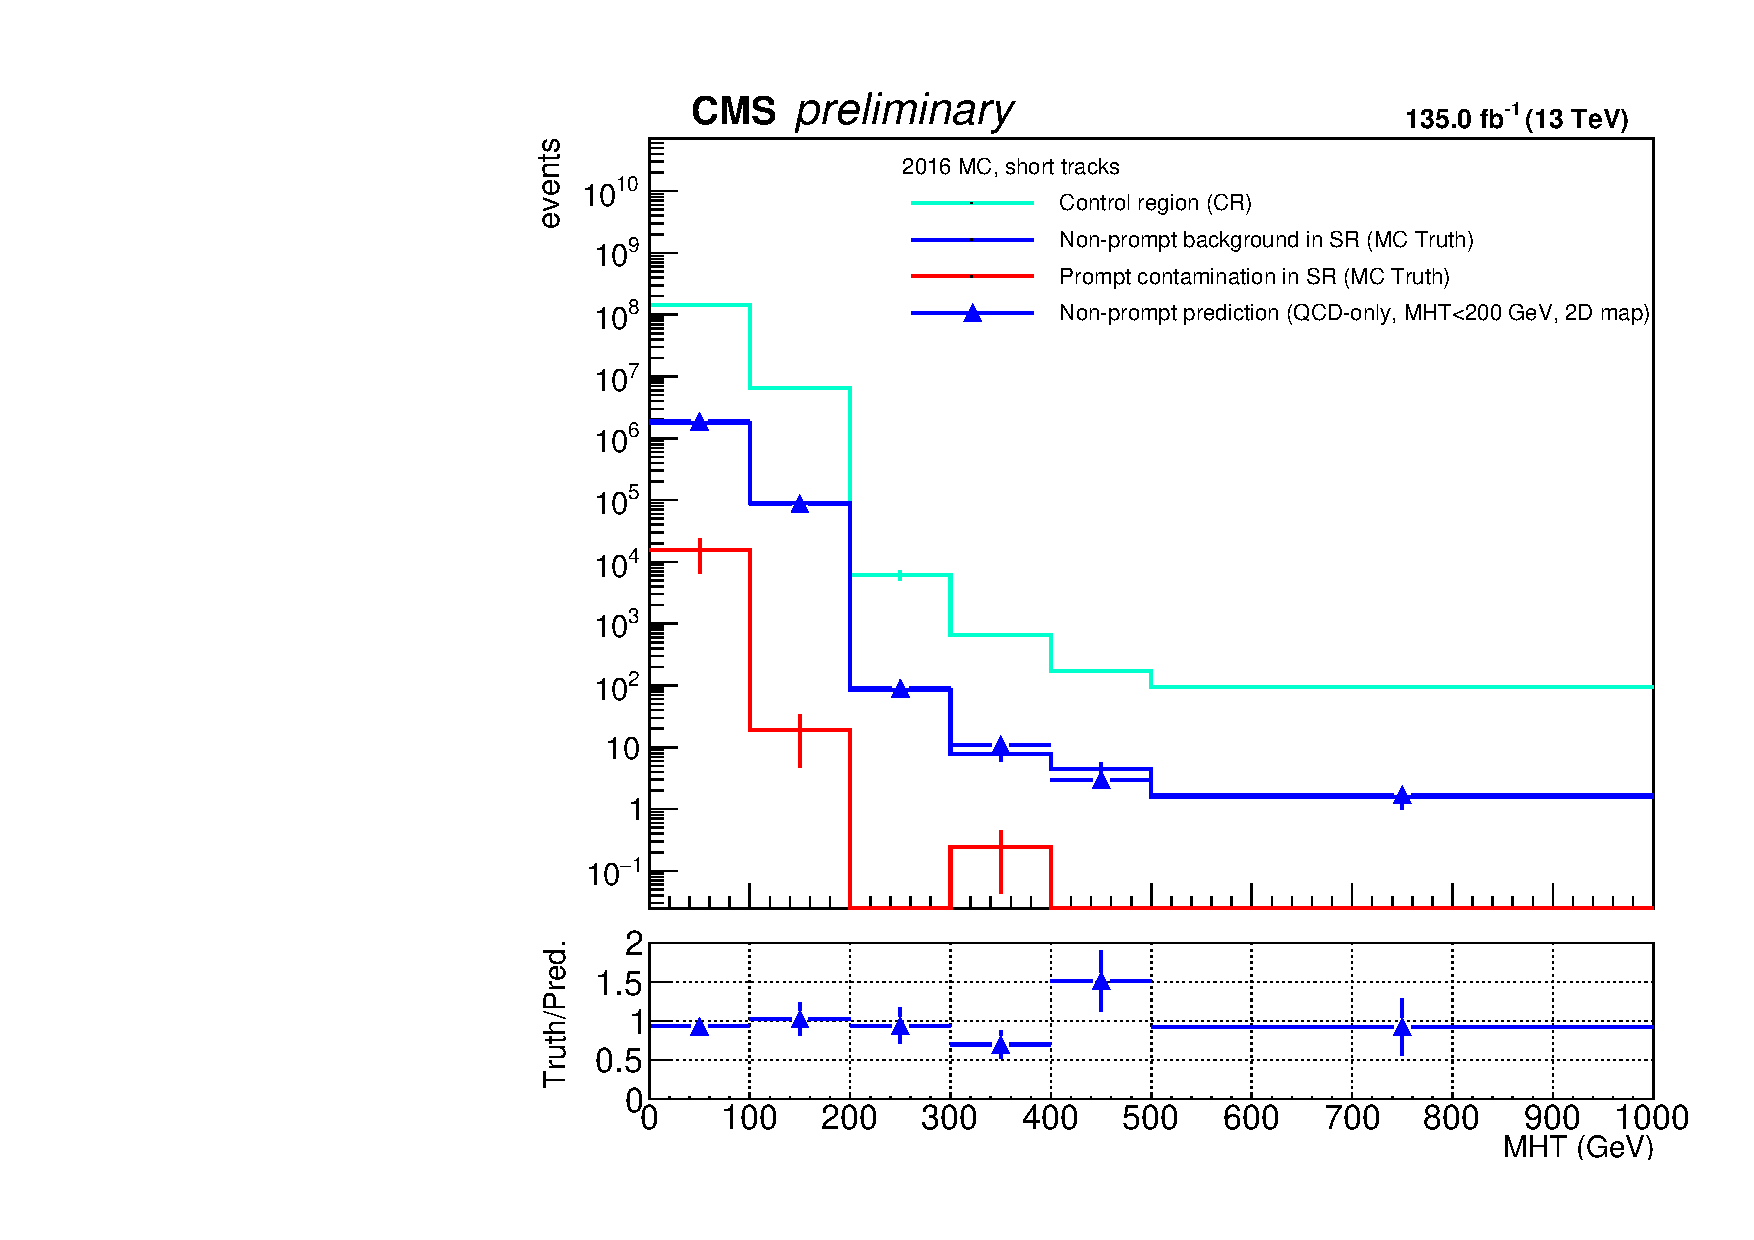
\includegraphics[width=.65\textwidth]{pdfs/prediction_Summer16_MHT_loose5_short_comparison_cr1.pdf}
\end{columns}
}



\frame{\frametitle{Incorporation of de/dx}
\scriptsize
\centering
\begin{columns}
\column{.5\textwidth}
\scriptsize
\begin{itemize}
\scriptsize
\item use pixel-only and strips-only ``harmonic2'' average ($I_h$)
\item compute mass using relation from \href{https://arxiv.org/abs/1101.1645}{arXiv:1101.1645 }
\begin{itemize}
\scriptsize
\item $I_{h} = K \frac{m^2}{p^2}+C$
\item $K = 2.579\pm0.001$ MeV $cm^{-1}$ $c^2$ and C = 2.557 $\pm$ 0.001 MeV $cm^{-1}$
\end{itemize}
\item calibration study of pixel de/dx \href{http://www.iexp.uni-hamburg.de/groups/pd/contents/index/index-124.html?q=theses/concept-search-heavy-stable-charged-particles-cms-tracking-system}{P. Asmuss master thesis\textbf{ link}}
\end{itemize}
Pursuing two approaches
\begin{enumerate}
\scriptsize
\item bin inclusively in jets and b-tagged jets, apply analysis MHT thresholds, fit mass distribution with a function
\item construct high/low mass template from ``prompt-like" and ``fake-like" control regions, use to split signal regions
\end{enumerate}
\column{.5\textwidth}
\centering
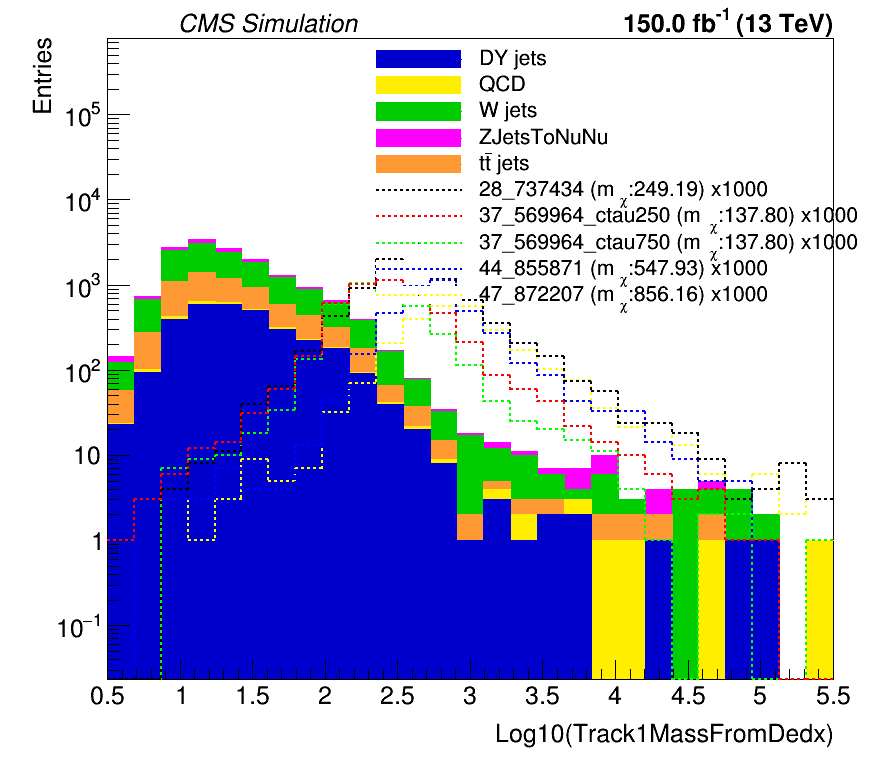
\includegraphics[width=.7\linewidth]{pdfs/10-Log10OfTrack1MassFromDedx_pMSSM28to47.png}\\
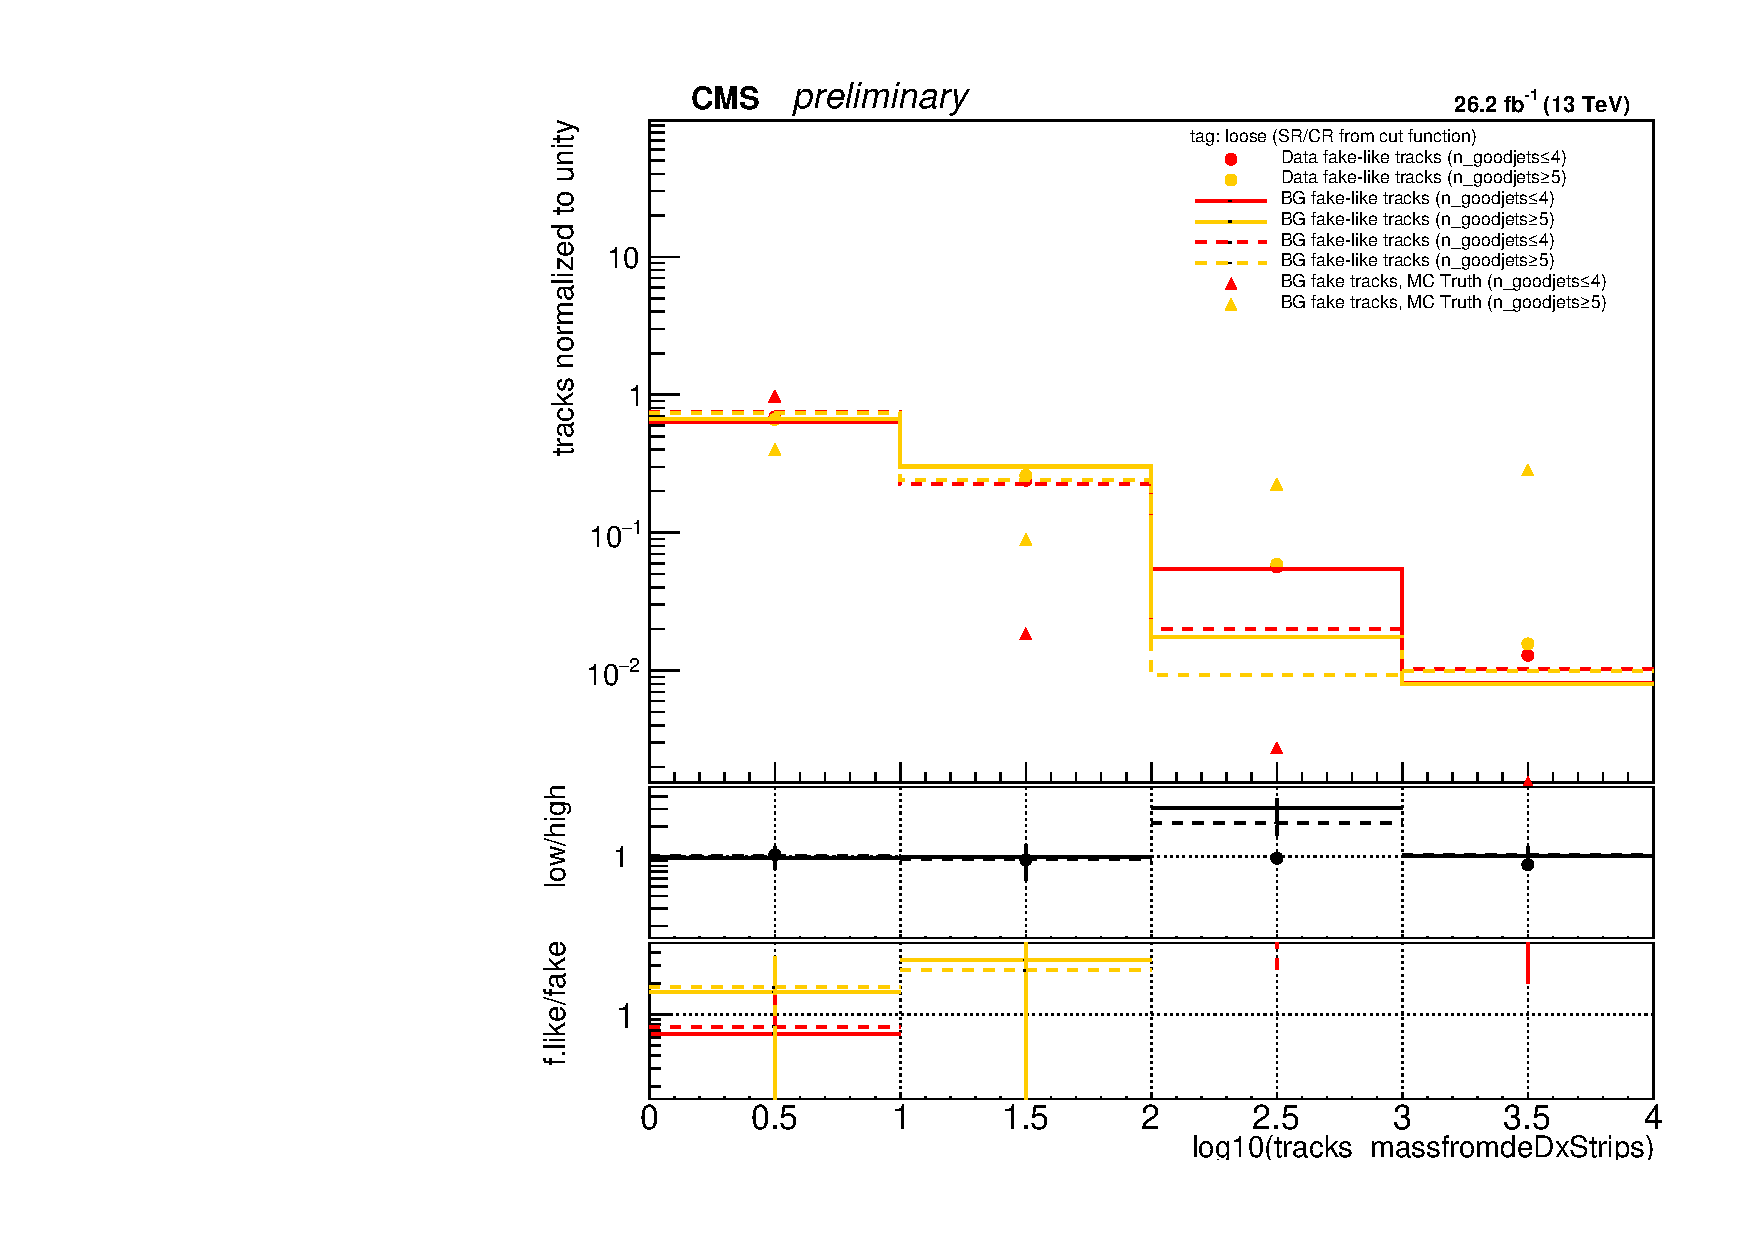
\includegraphics[width=.7\linewidth]{pdfs/11-waterfall_fake_loose3_highlowJets.pdf}
\end{columns}
}



\frame{\frametitle{Status of signal}
\centering
\begin{columns}
\column{.5\textwidth}
\begin{itemize}
\scriptsize
\item We requested several samples in the spring (examples in next couple of slides)
\item Samples were not produced for various reasons
\item One factor is that FastSim now produces AOD's that contain the de/dx collections (now added)
\item We would like to re-start these campaigns as soon as possible
\end{itemize}
\centering
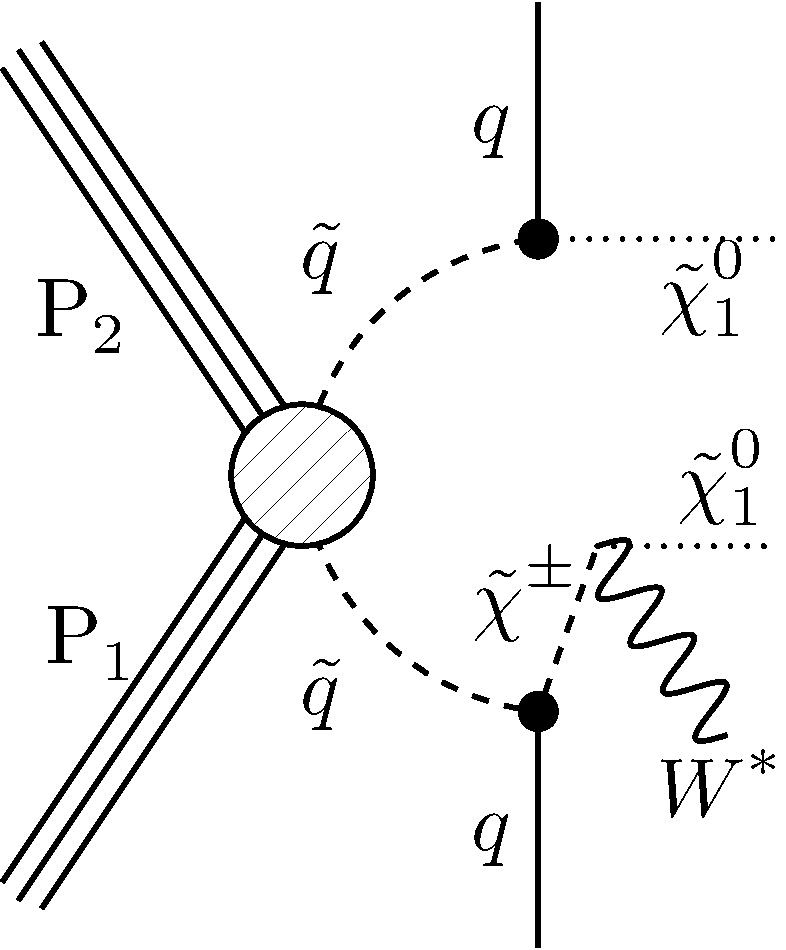
\includegraphics[width=.35\linewidth]{pdfs/12-1b_T3wqq}
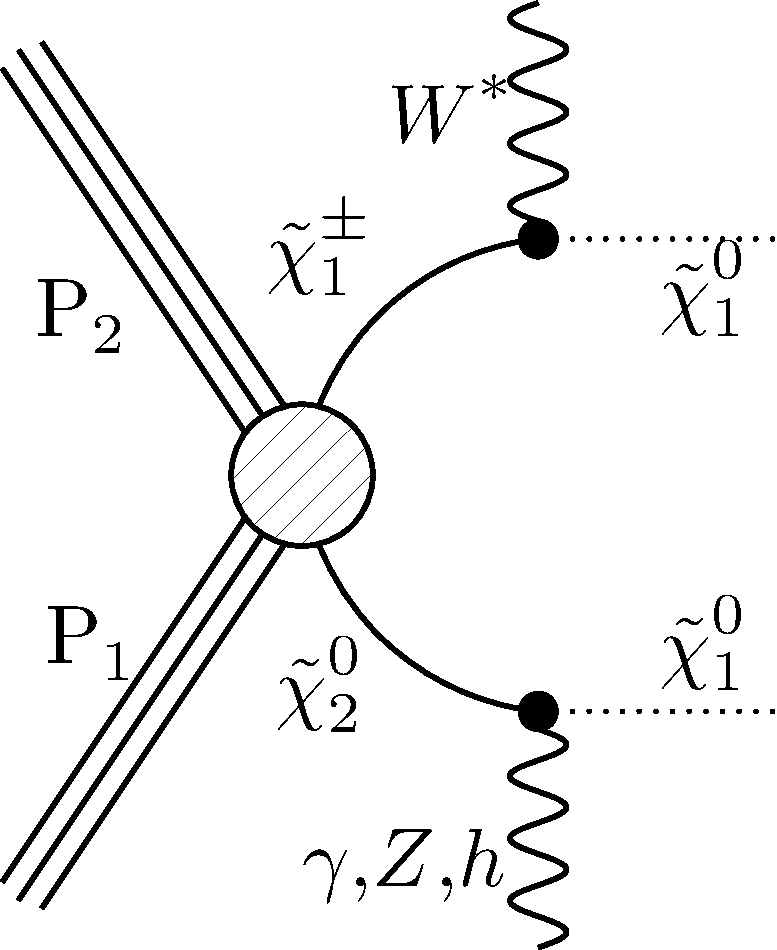
\includegraphics[width=.35\linewidth]{pdfs/13-103b_TChiWB}
\column{.5\textwidth}
\centering
\scriptsize
plots of fastsim de/dx
\end{columns}
}

\frame{\frametitle{Model T1btbLL (requested)}
\begin{center}
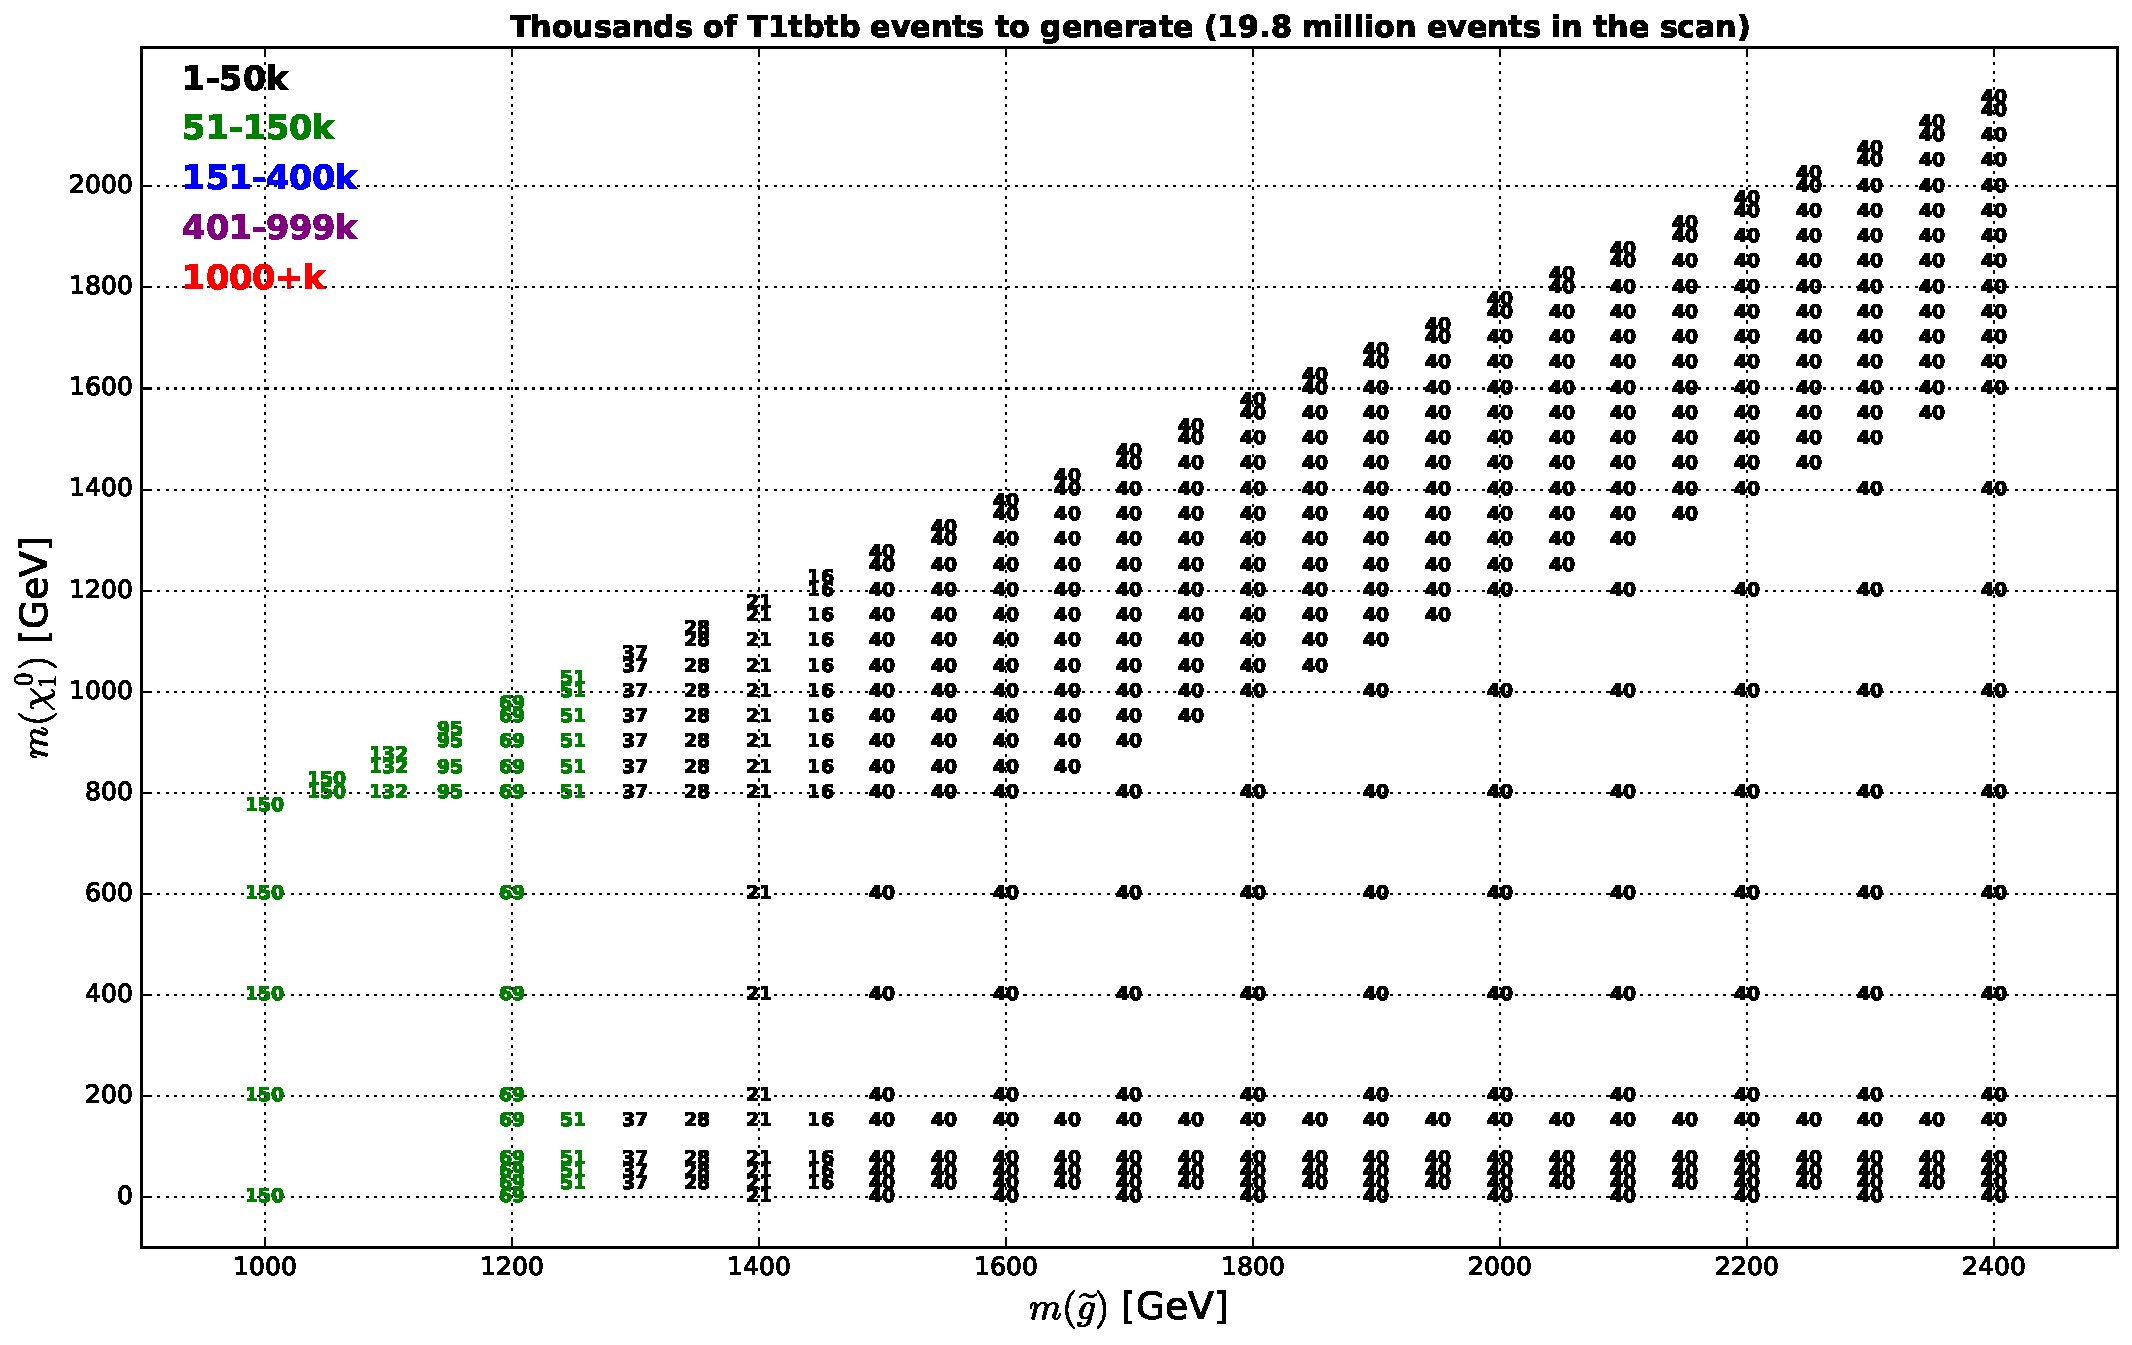
\includegraphics[width=\linewidth]{pdfs/14-T1tbtb_events.pdf}
\end{center}
}

\frame{\frametitle{Model T1tbtb (requested)}
\begin{center}
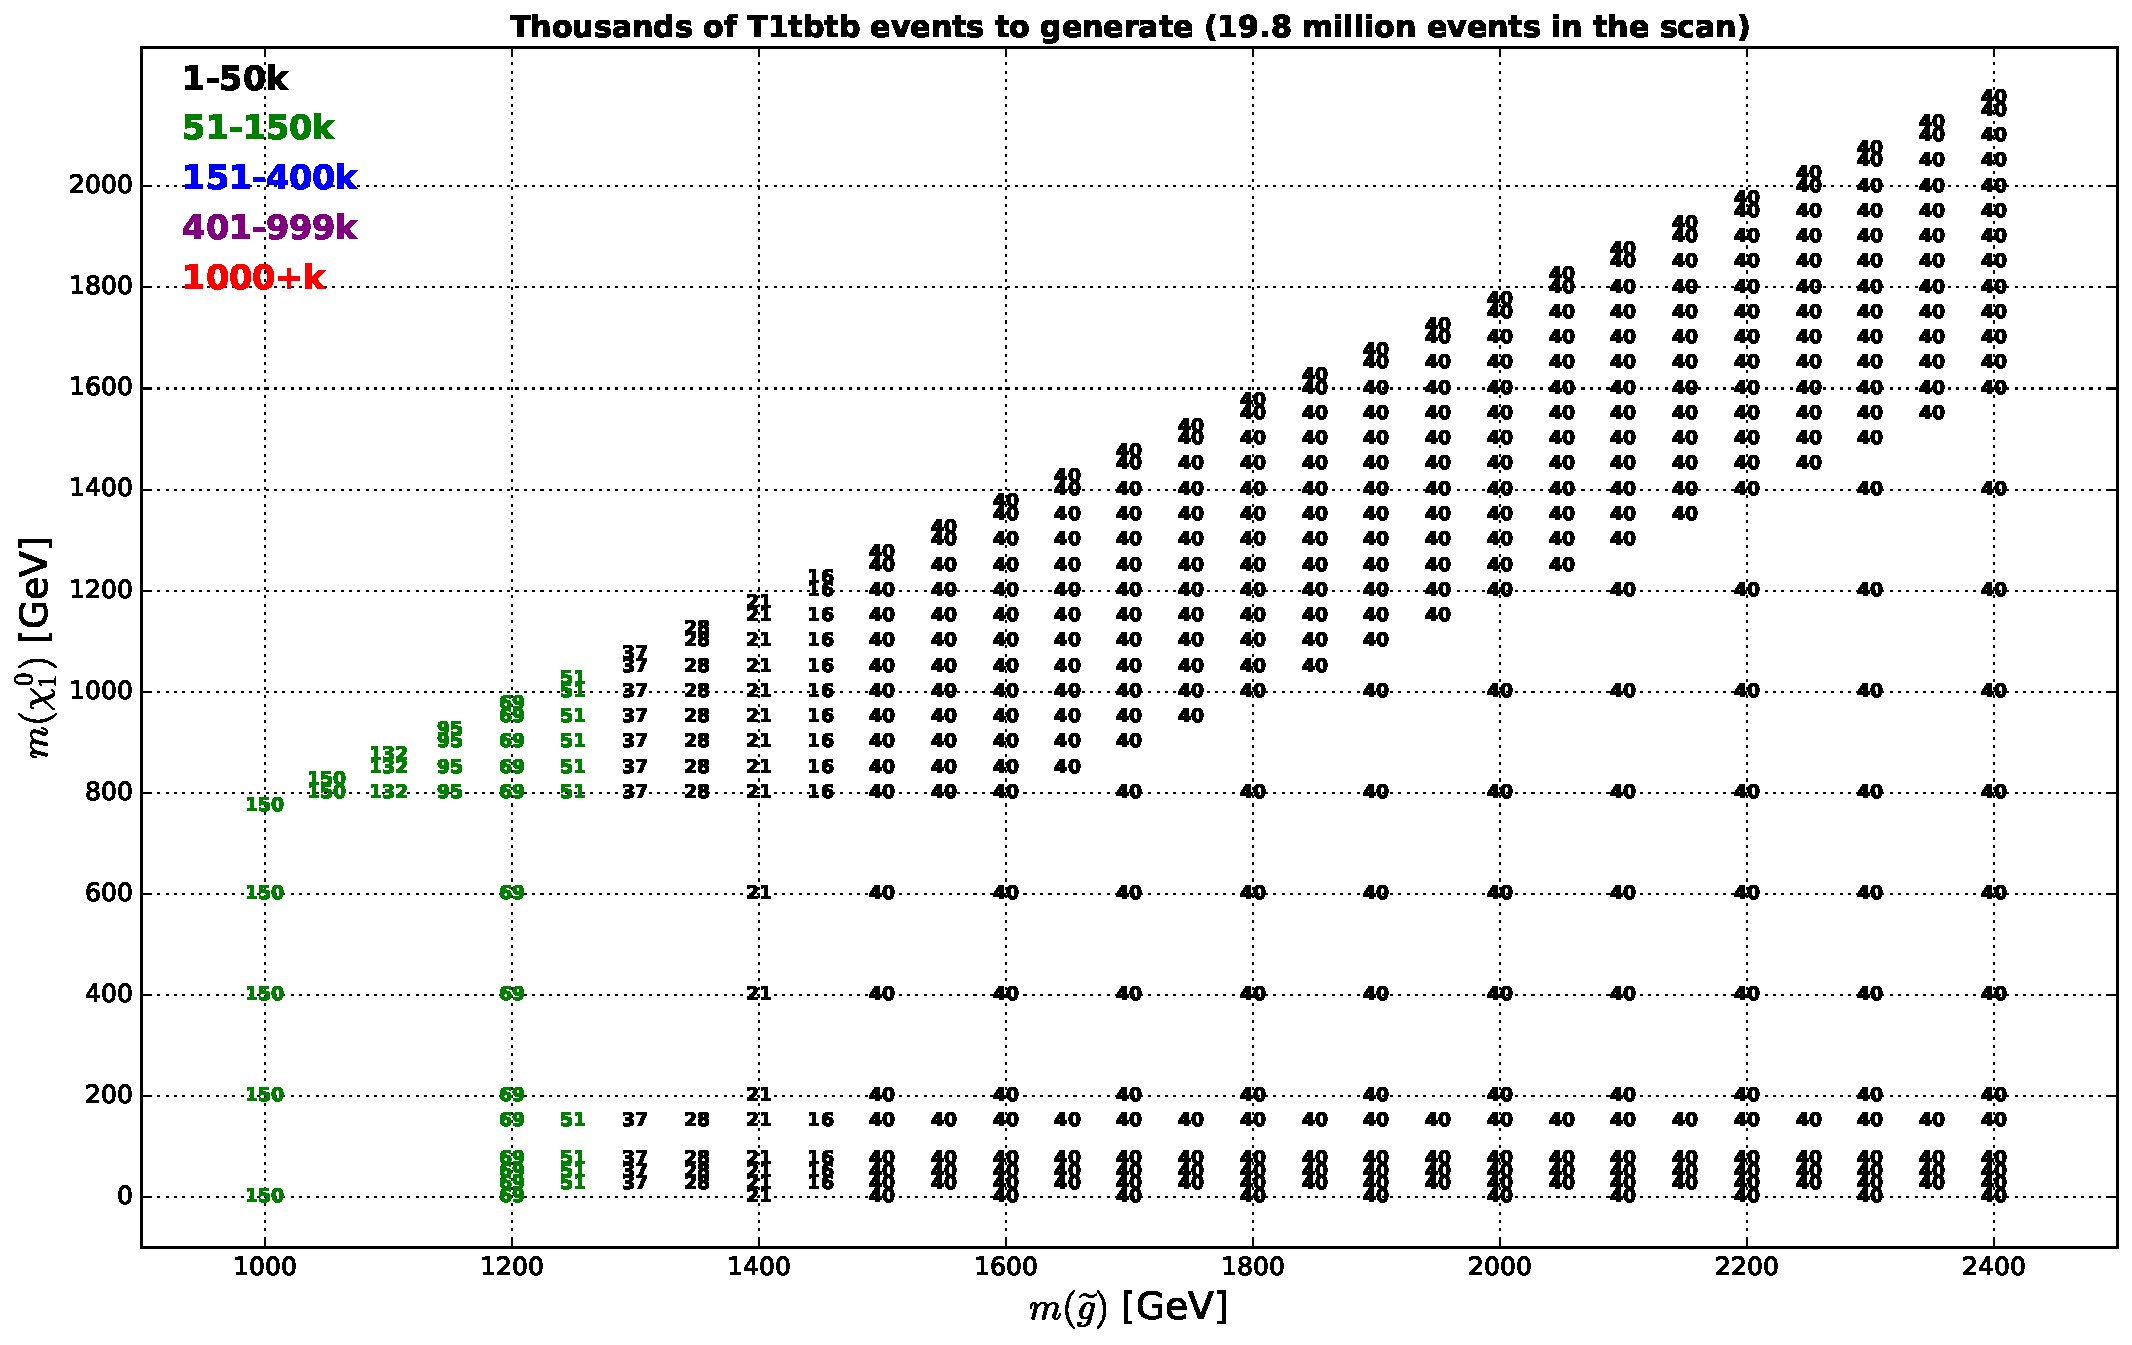
\includegraphics[width=\linewidth]{pdfs/15-T1tbtb_events.pdf}
\end{center}
}


\frame{\frametitle{Conclusions and outlook}
\small
\begin{itemize}
\scriptsize
\item Background methods show improvement in 2016 and 2017 MC
\item Dropping muon veto should help pick up sensitivity to some long-lived scenarios
\item Indications that mass(de/dx) is invariant w.r.t. event topology, differs between fake and prompt tracks
\item Still need to study masks for 2017 and 2018 data
\item Still need to re-do data-validation studies with the new tag
\end{itemize}
}




\appendix
\backupbegin

\frame{\frametitle{}
\begin{center}
\huge{Backup}
\end{center}
}




\frame{\frametitle{Prompt background: $\kappa$}
\begin{columns}
\column{.5\linewidth}
\centering
\textbf{electrons}
\column{.5\linewidth}
\centering
\textbf{muons}
\end{columns}
\vspace{0.2cm}
\begin{columns}
\column{.25\linewidth}
\scriptsize
\centering
short - barrel\\
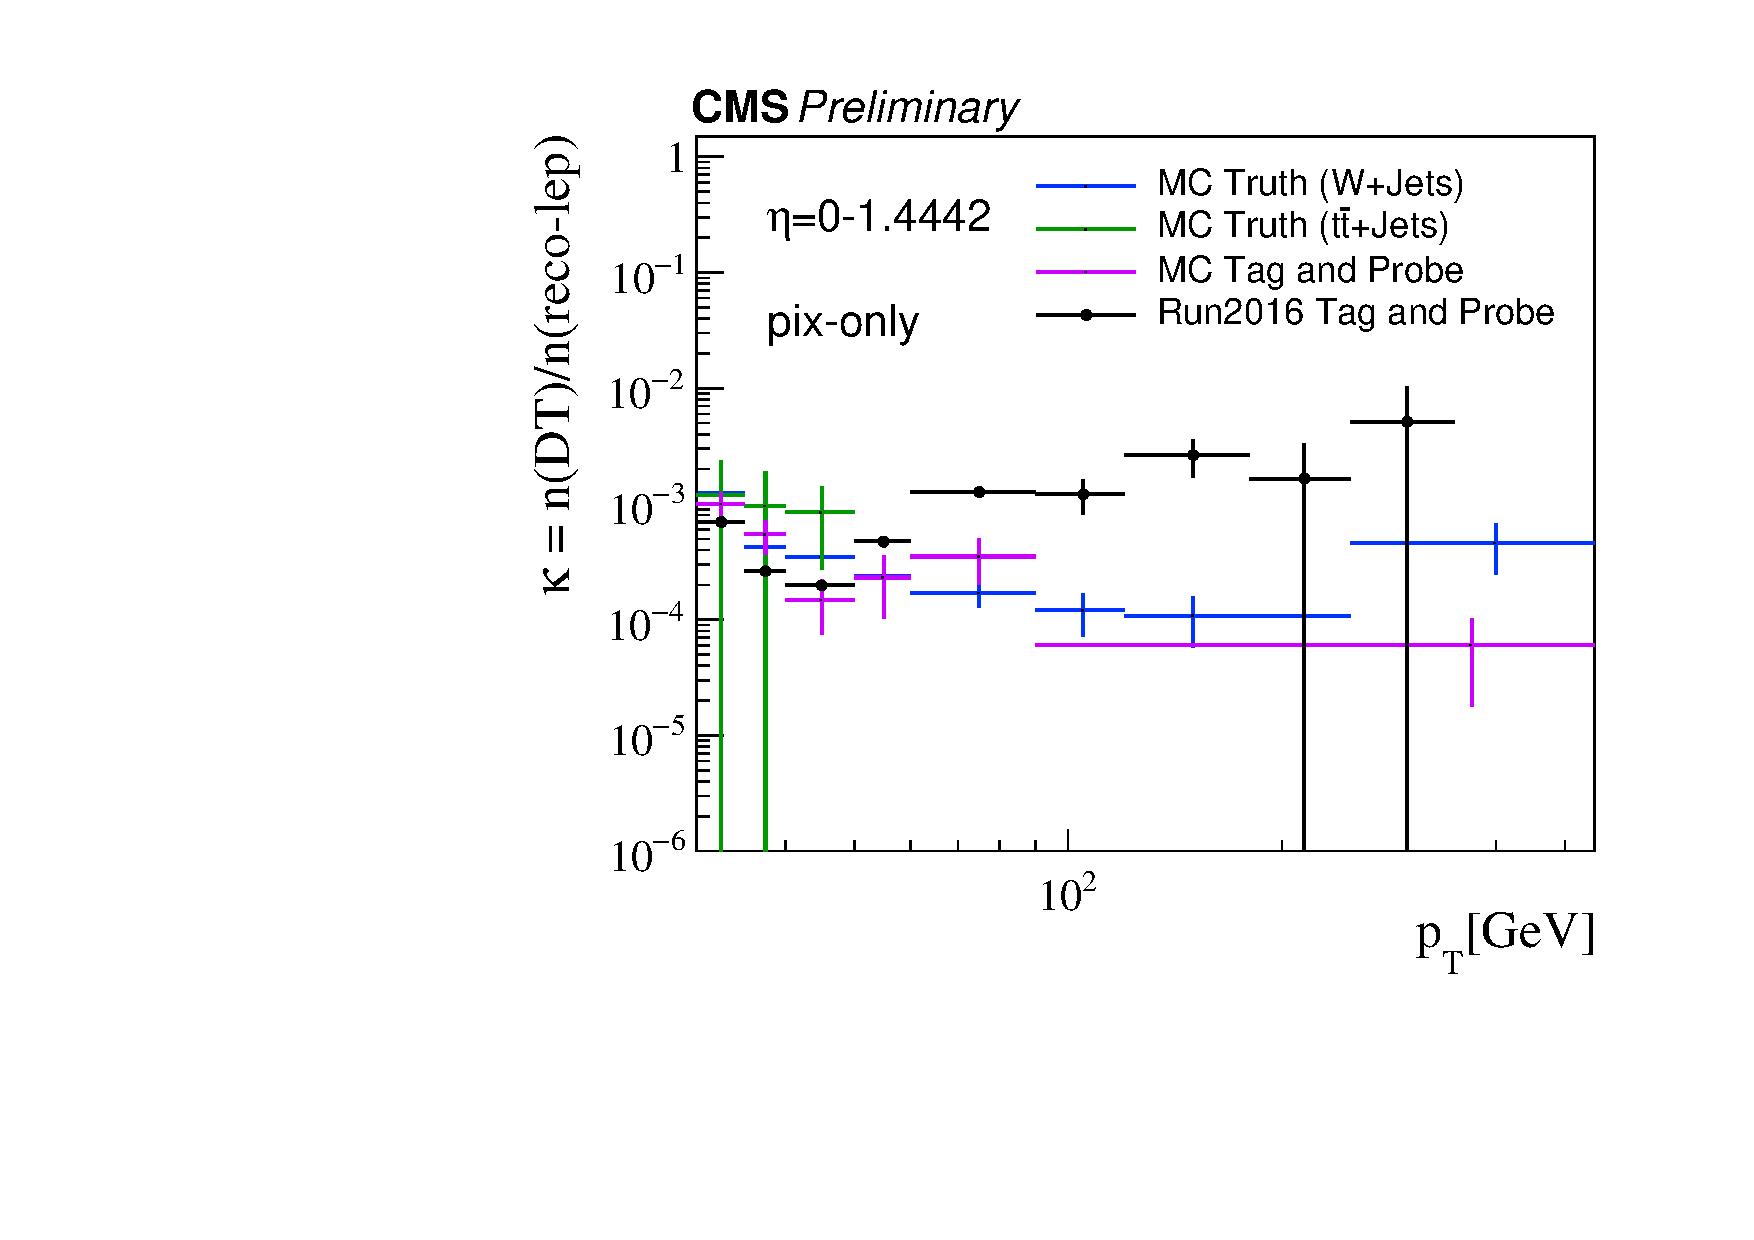
\includegraphics[width=1\linewidth]{pdfs/16-kappaElProbePtKappa_eta0to1p4442_PixOnly.pdf}\\
long  - barrel\\
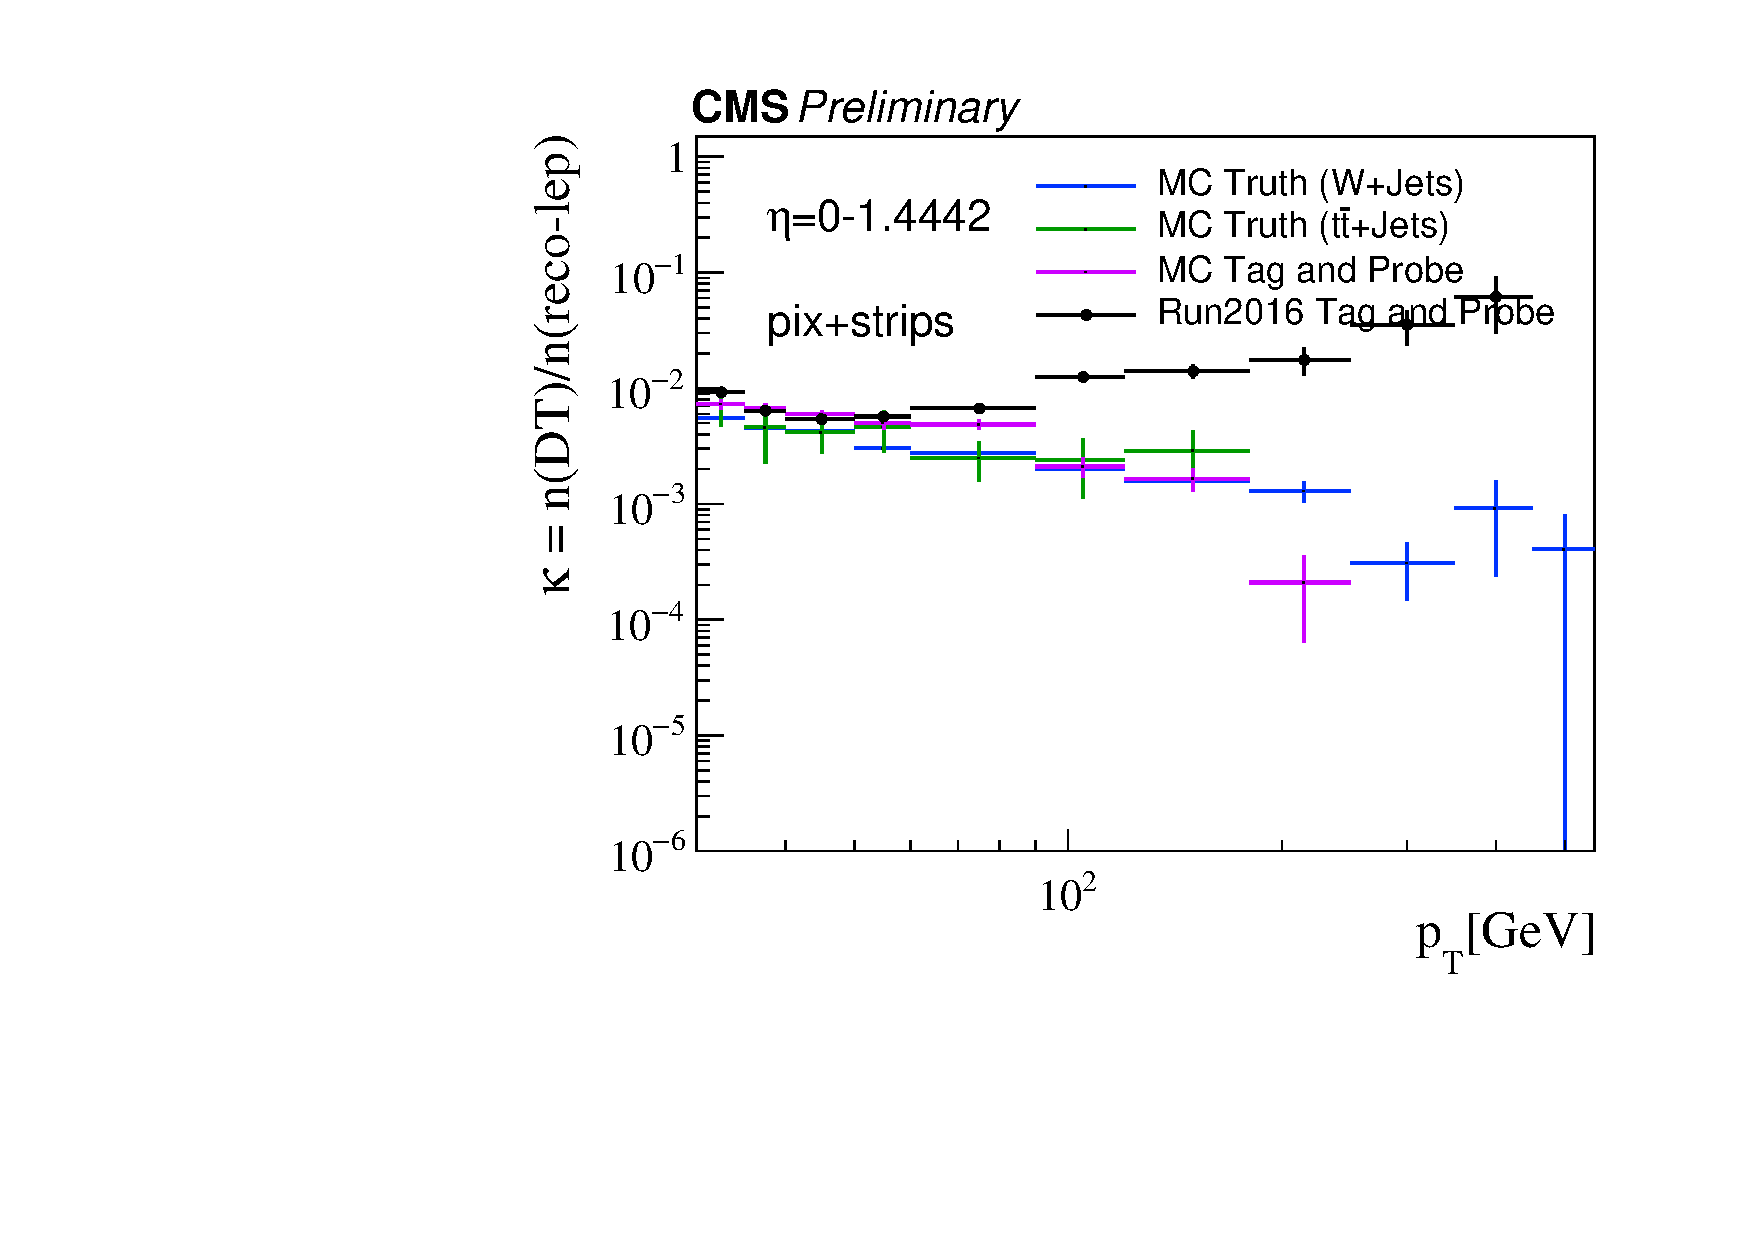
\includegraphics[width=1\linewidth]{pdfs/17-kappaElProbePtKappa_eta0to1p4442_PixAndStrips.pdf}
\column{.25\linewidth}
\scriptsize
\centering
short - endcap\\
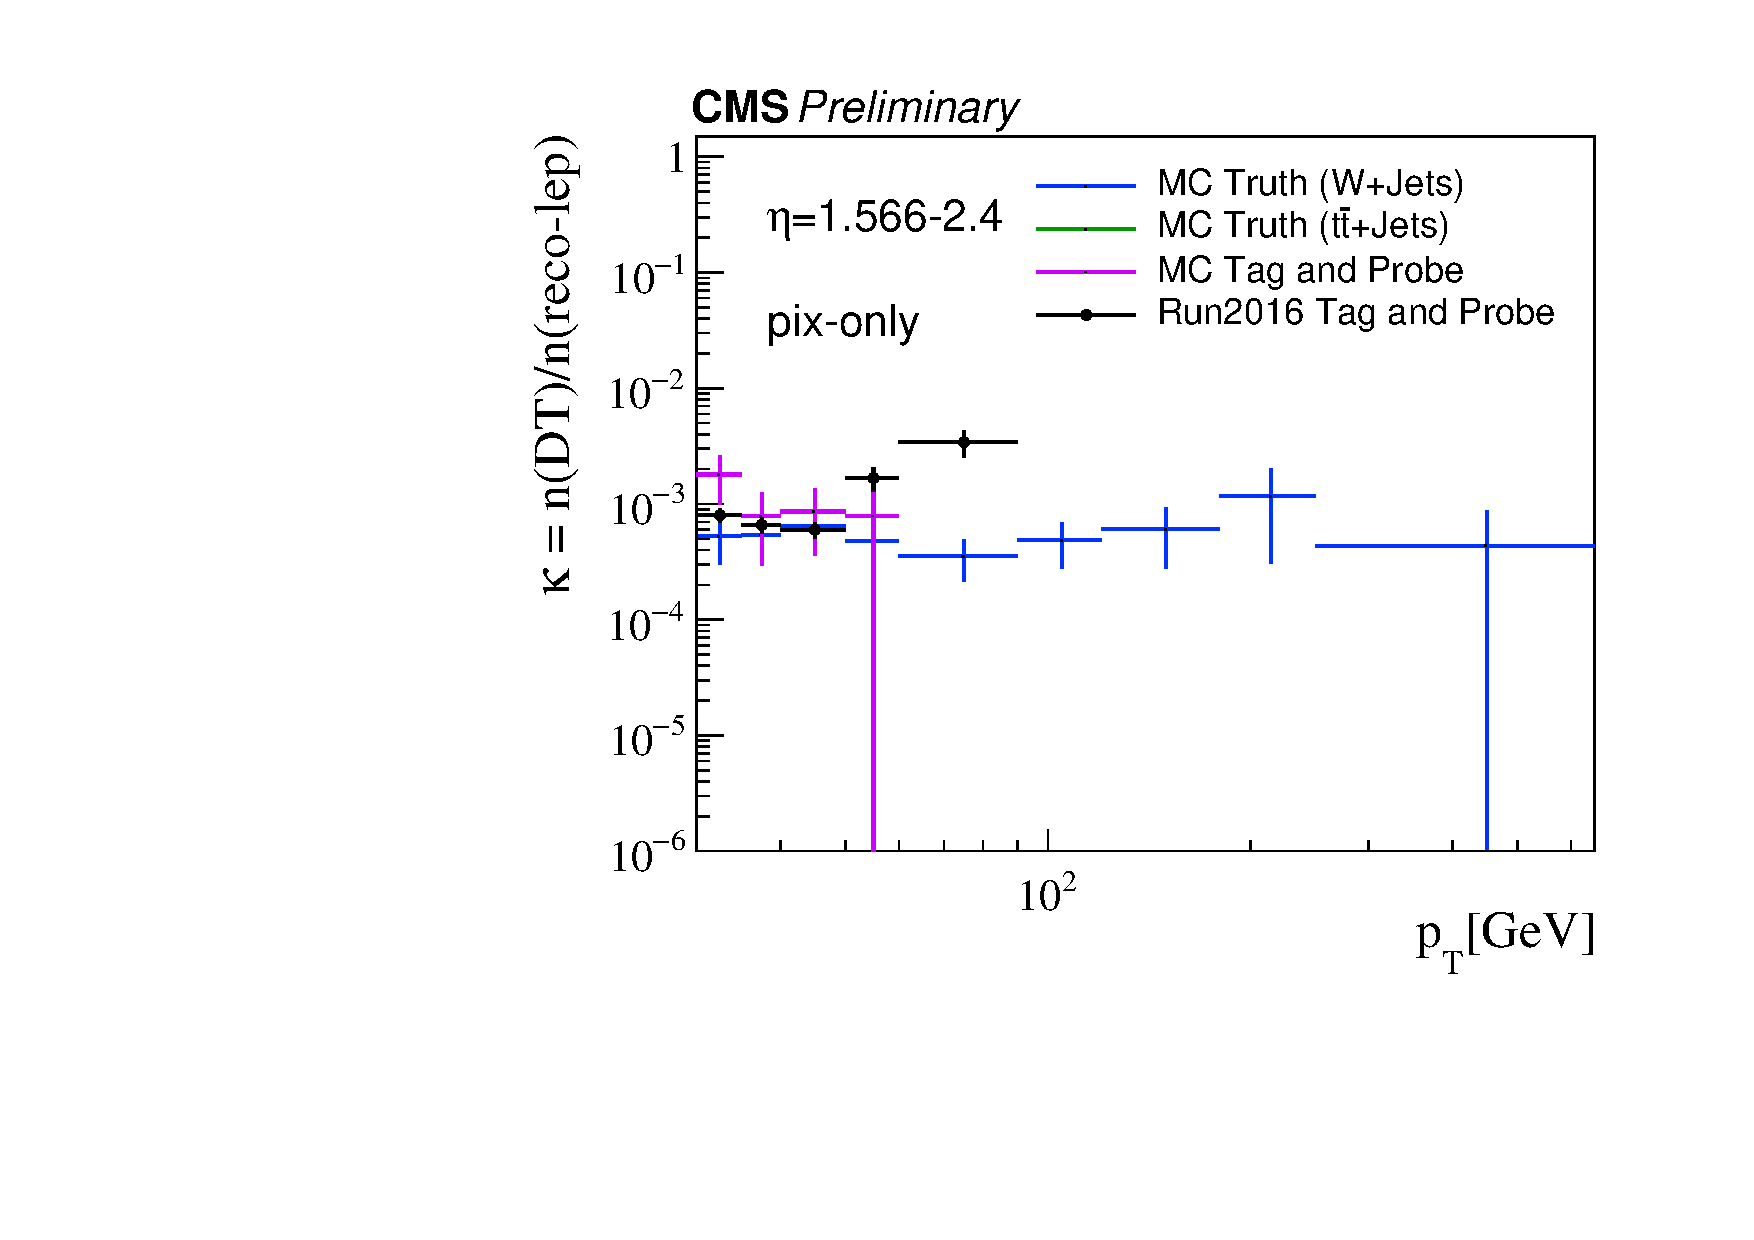
\includegraphics[width=1\linewidth]{pdfs/18-kappaElProbePtKappa_eta1p566to2p4_PixOnly.pdf}\\
long - endcap\\
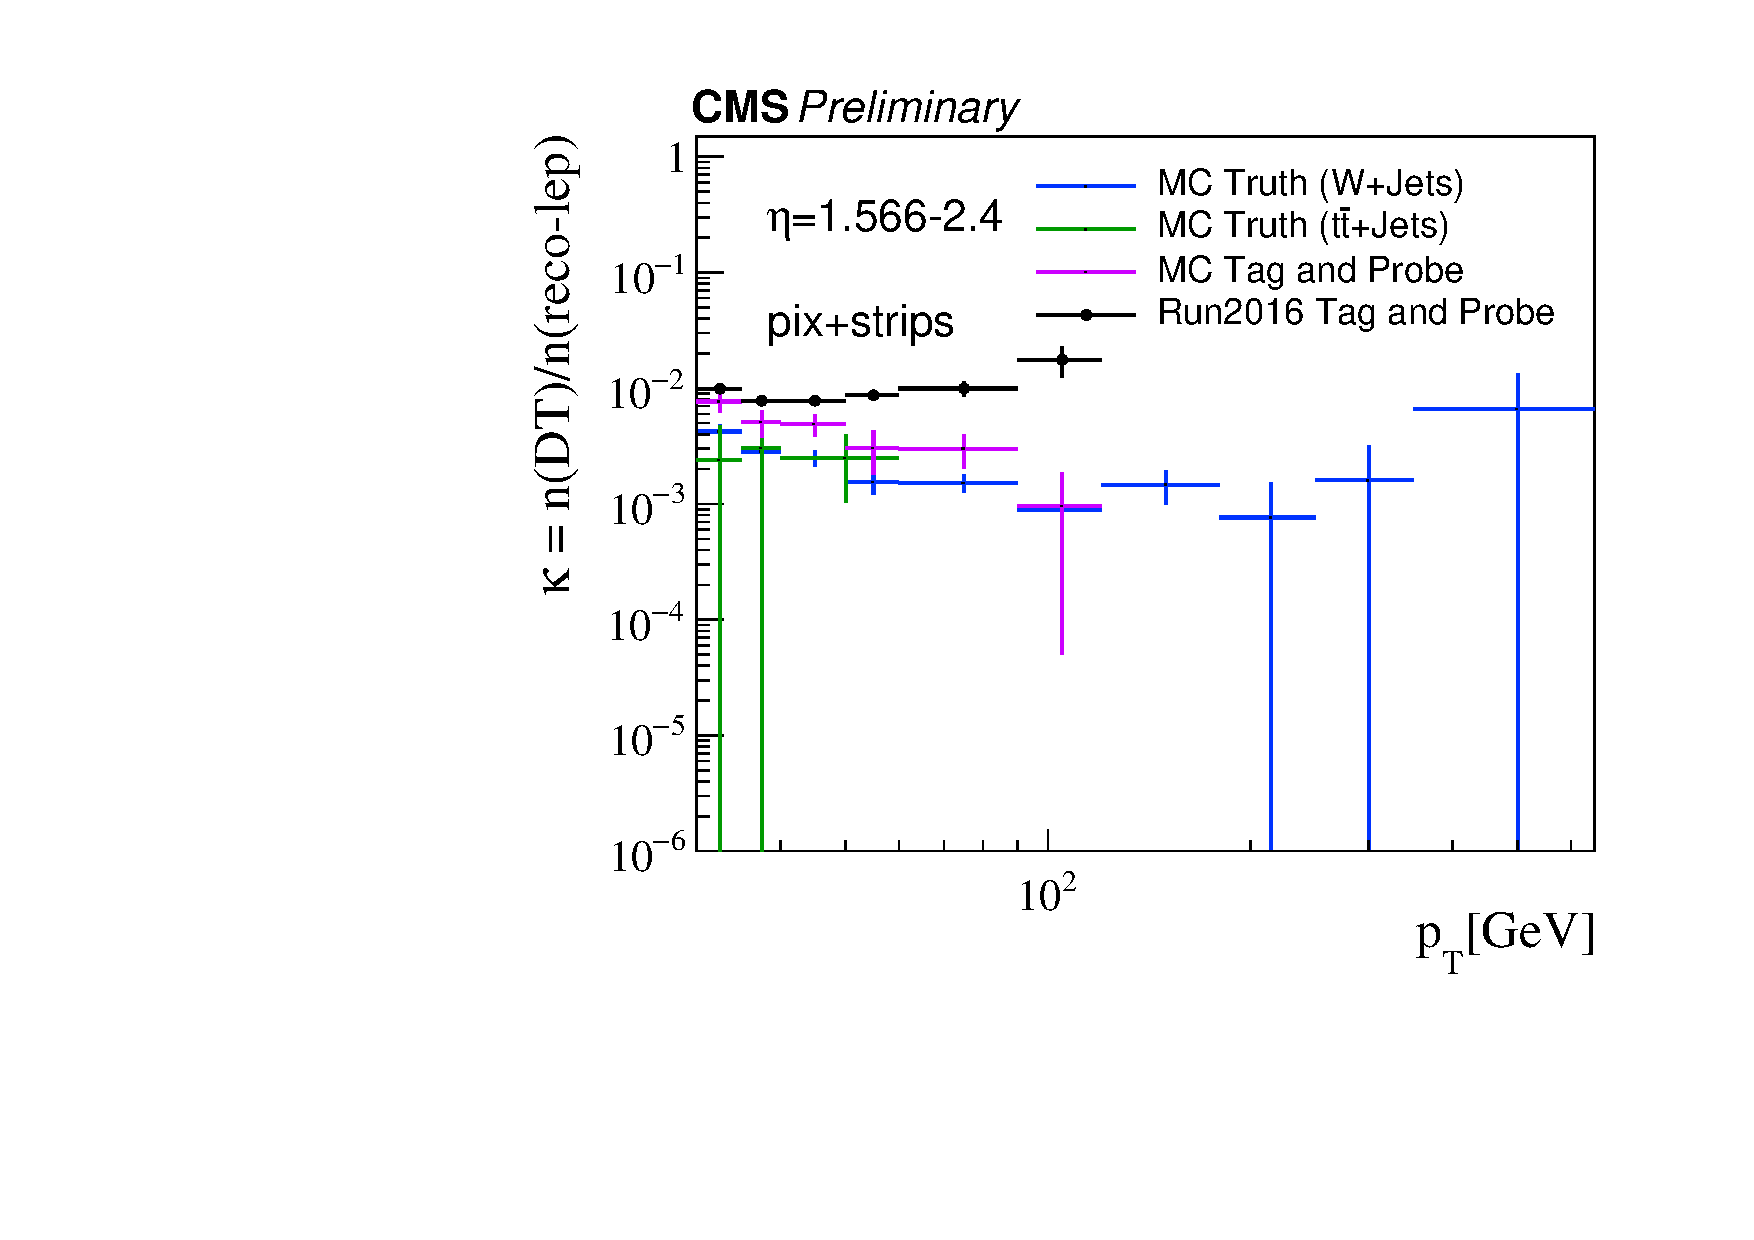
\includegraphics[width=1\linewidth]{pdfs/19-kappaElProbePtKappa_eta1p566to2p4_PixAndStrips.pdf}
\column{.25\linewidth}
\scriptsize
\centering
short - barrel\\
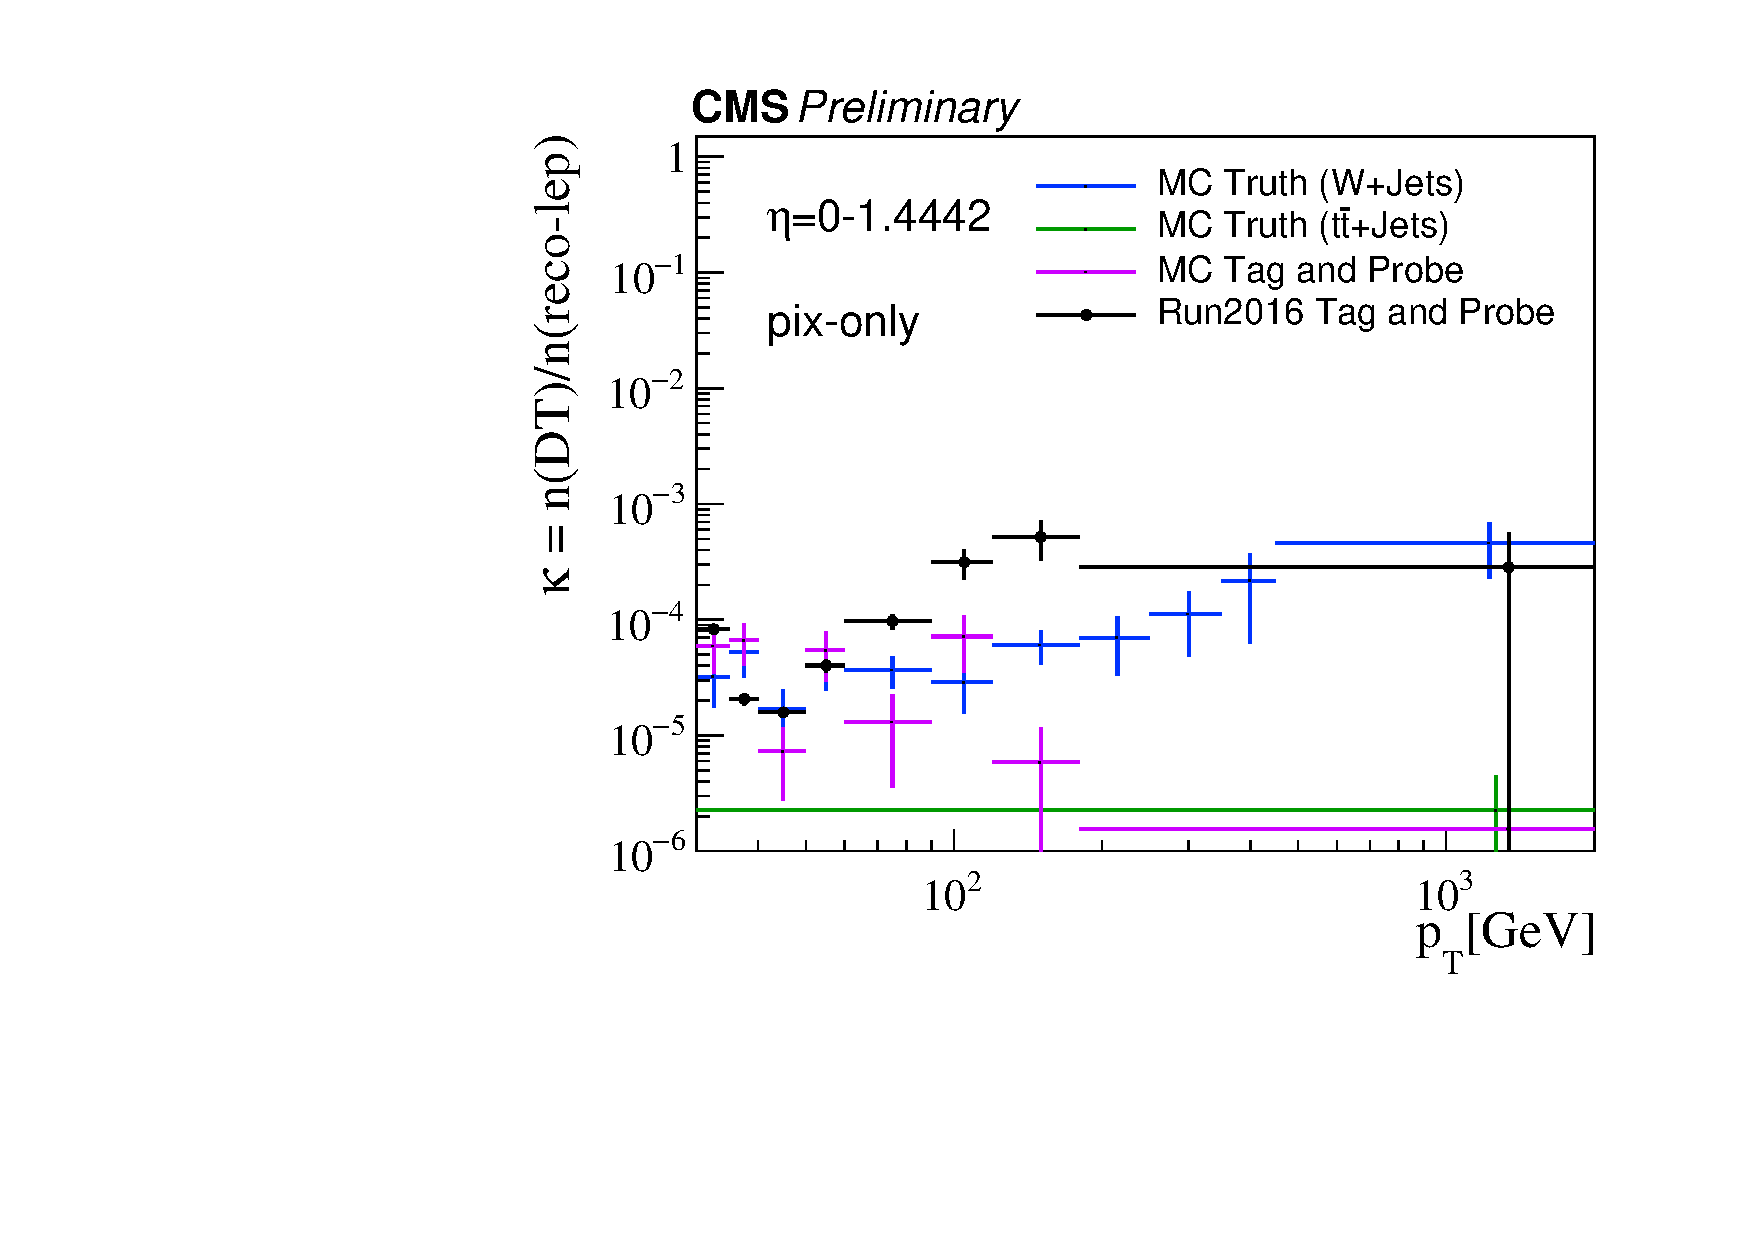
\includegraphics[width=1\linewidth]{pdfs/20-kappaMuProbePtKappa_eta0to1p4442_PixOnly.pdf}\\
long  - barrel\\
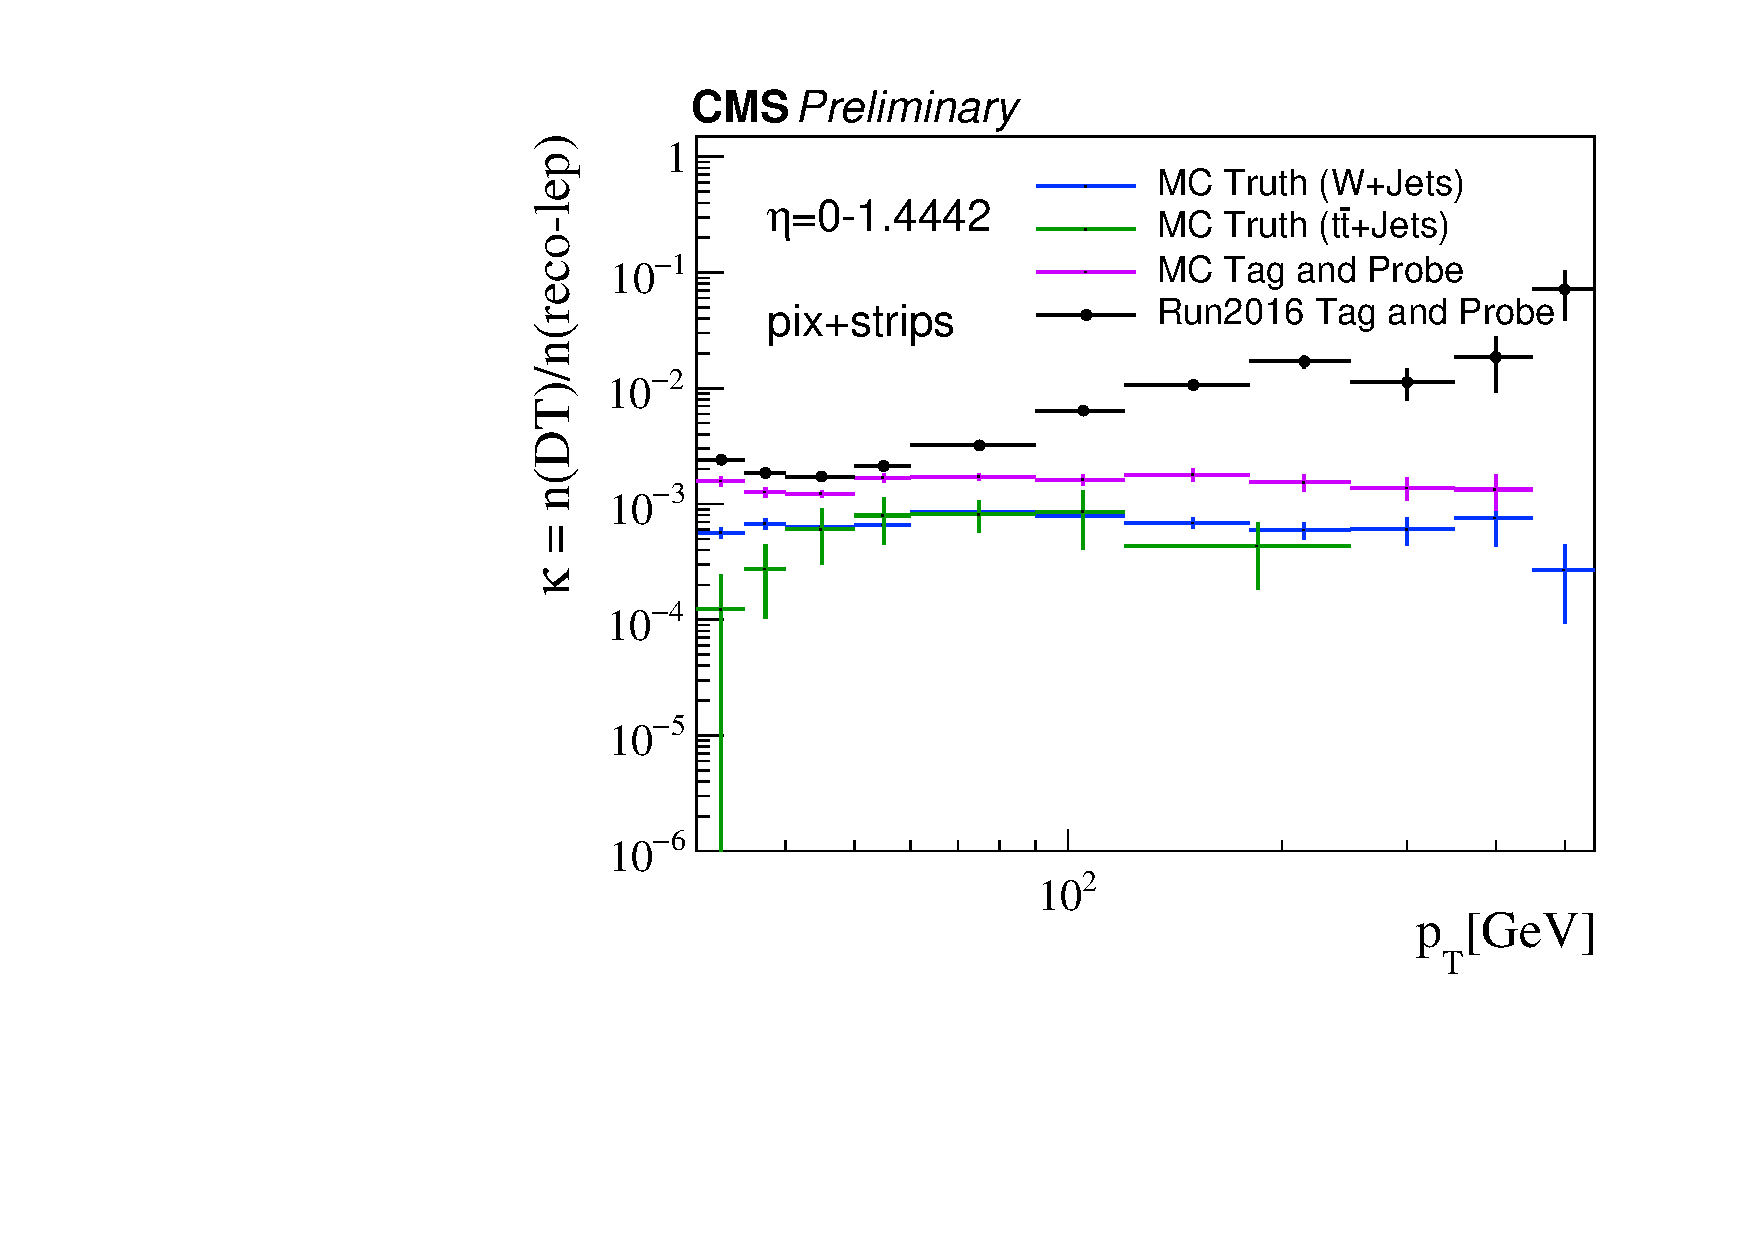
\includegraphics[width=1\linewidth]{pdfs/21-kappaMuProbePtKappa_eta0to1p4442_PixAndStrips.pdf}
\column{.25\linewidth}
\scriptsize
\centering
short - endcap\\
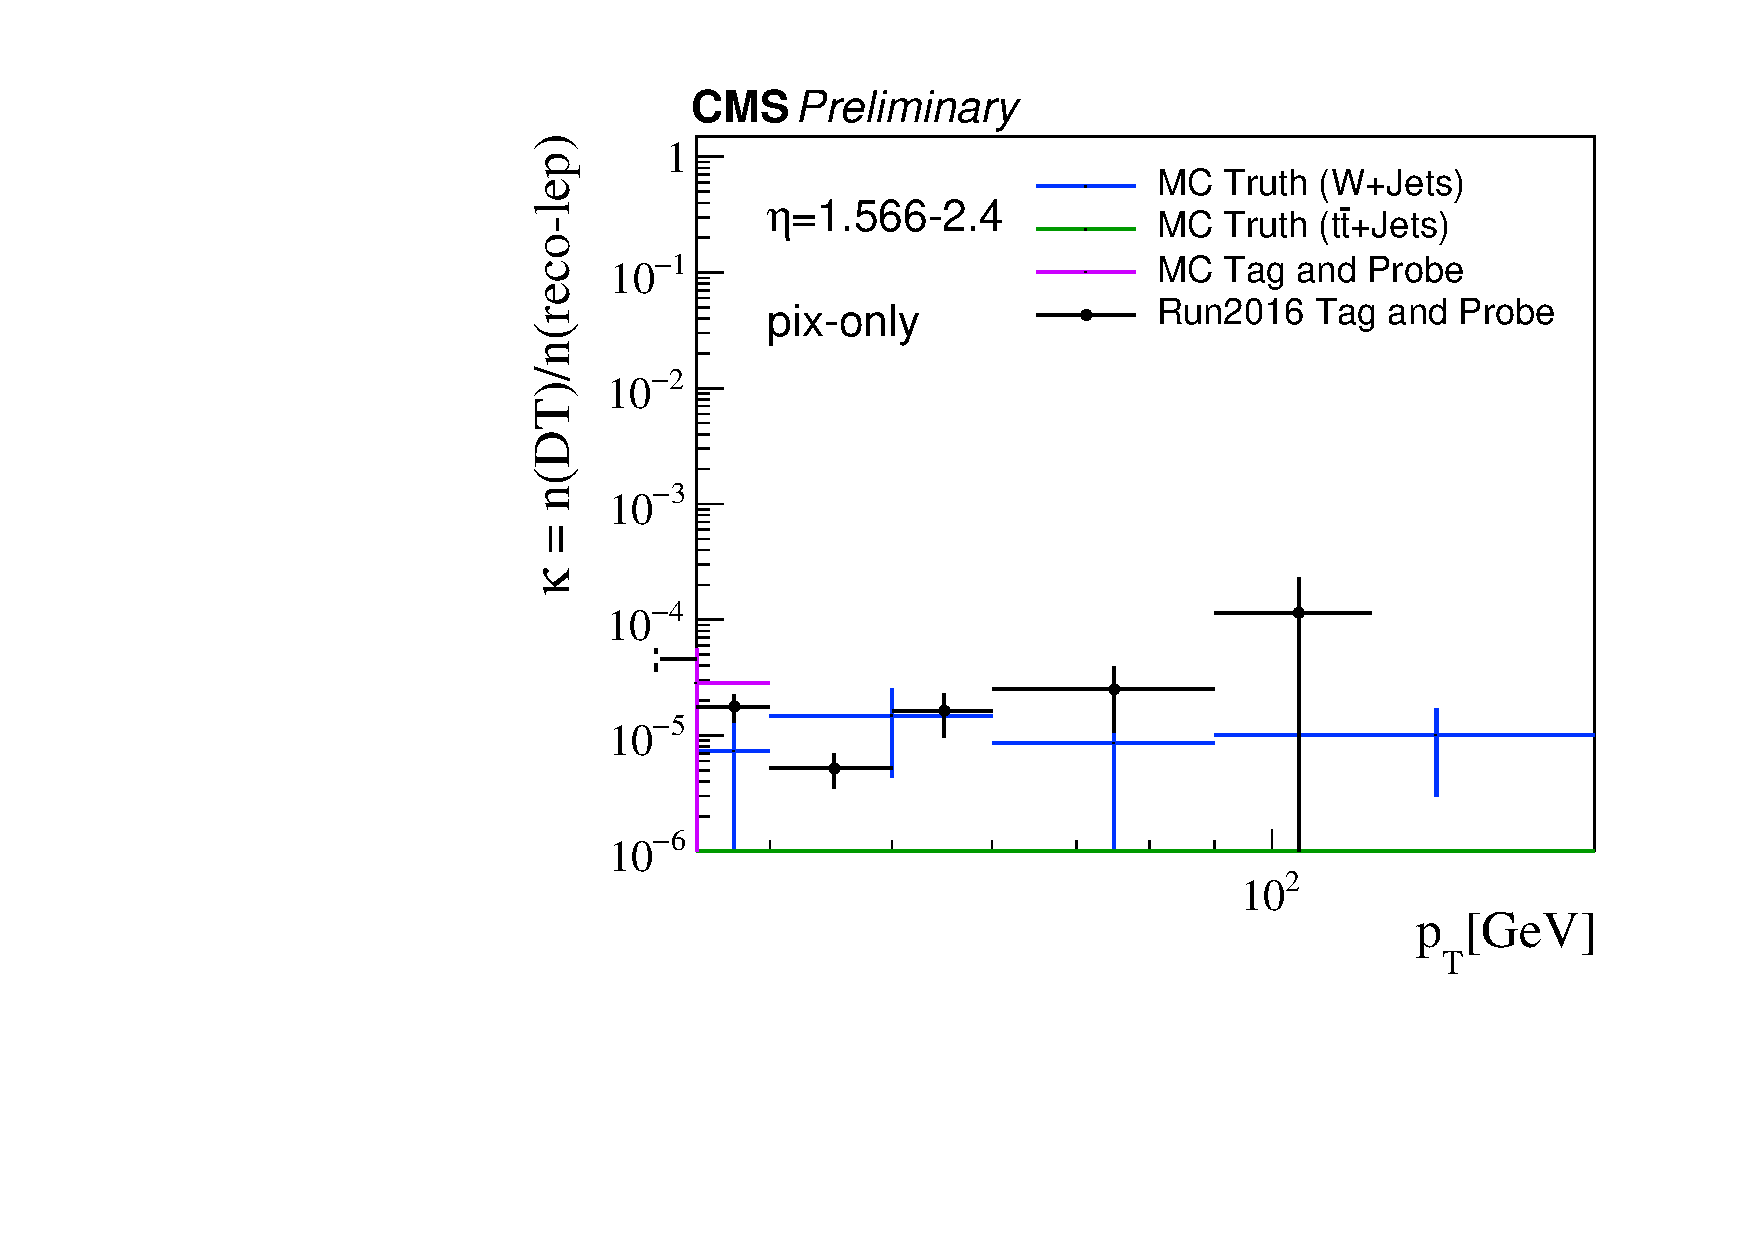
\includegraphics[width=1\linewidth]{pdfs/22-kappaMuProbePtKappa_eta1p566to2p4_PixOnly.pdf}\\
long - endcap\\
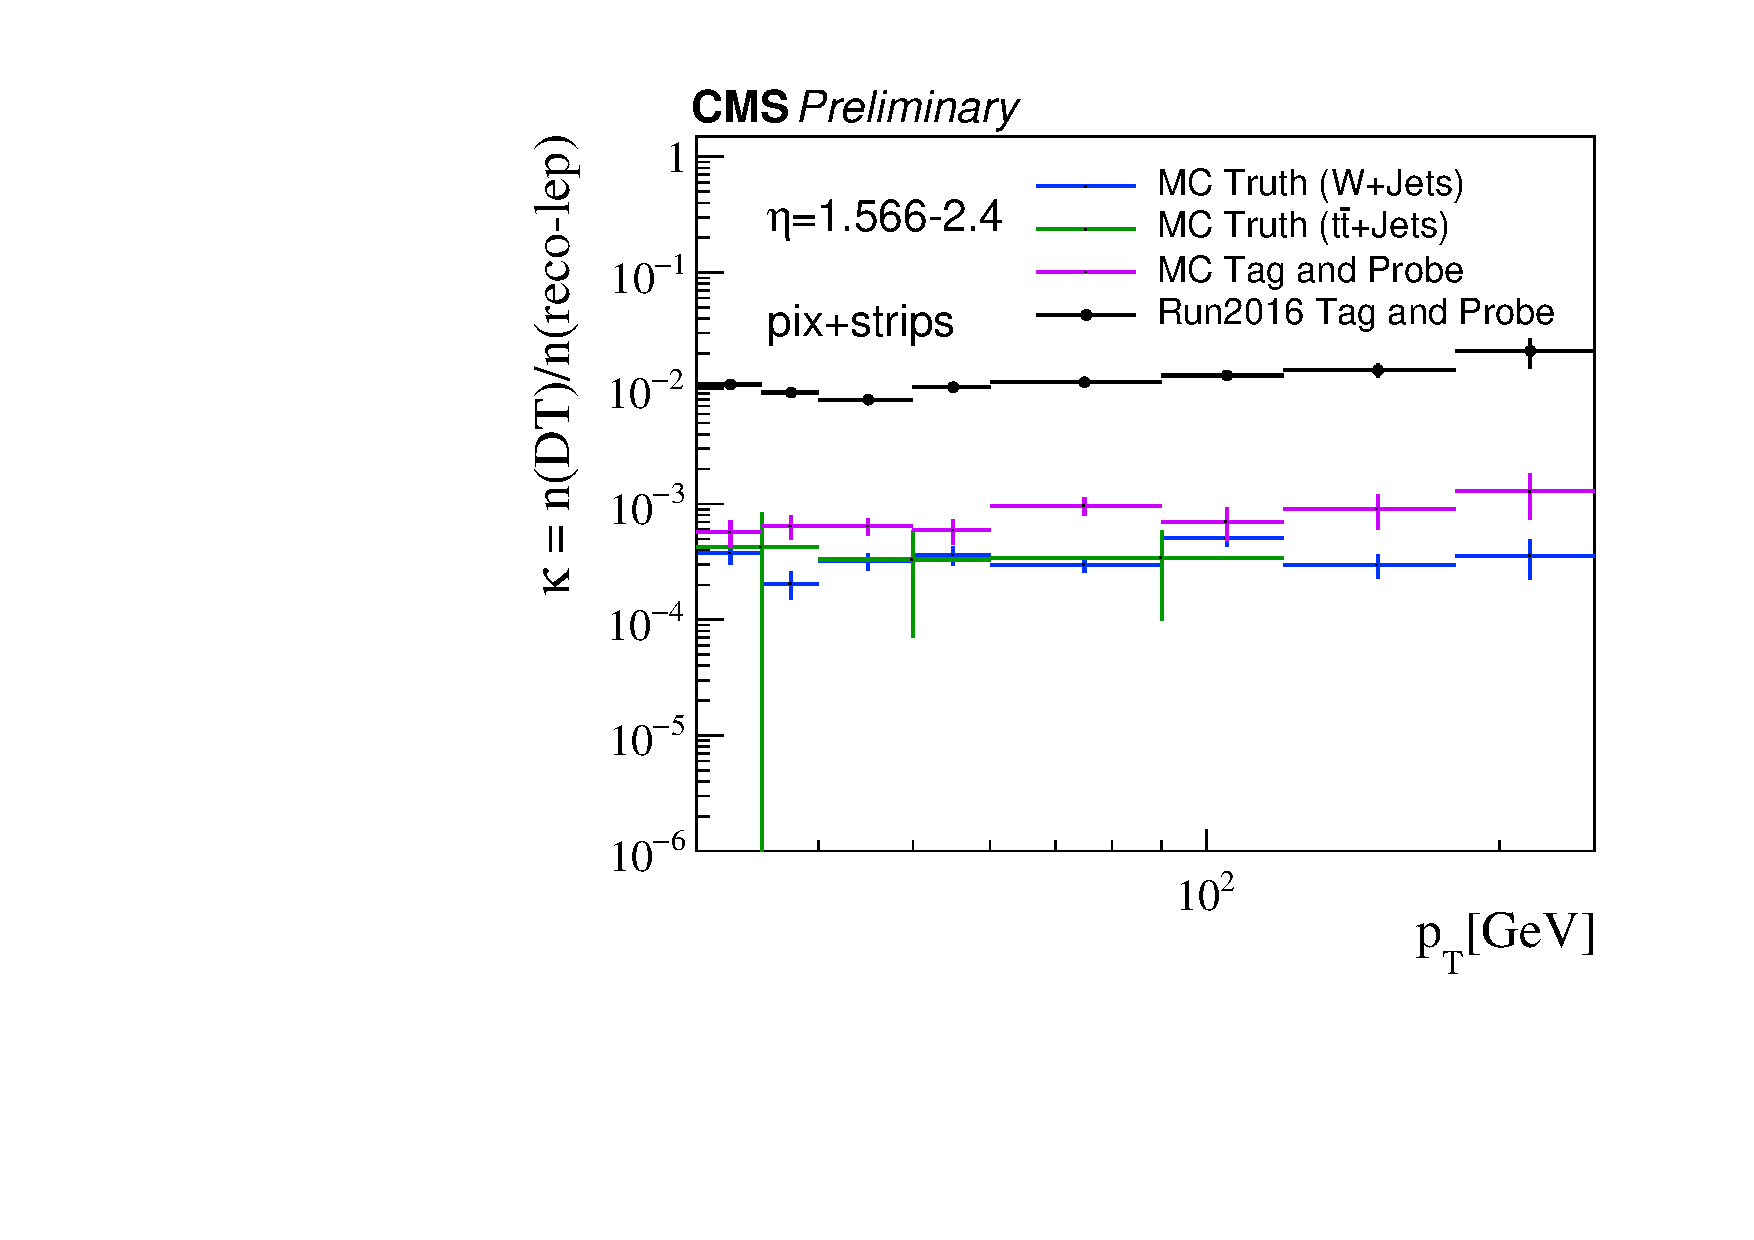
\includegraphics[width=1\linewidth]{pdfs/23-kappaMuProbePtKappa_eta1p566to2p4_PixAndStrips.pdf}
\end{columns}
\vspace{.2cm}
\scriptsize
\textbf{black}: tag/probe in data; {\color{violet} violet: tag/probe in MC}; {\color{blue} blue: MC truth (W+Jets)}; {\color{ForestGreen} green: MC truth ($t\bar{t}$+jets); }
}


\frame{\frametitle{}
\vspace{-.16cm}
\centering
\textbf{smearing functions (global)}
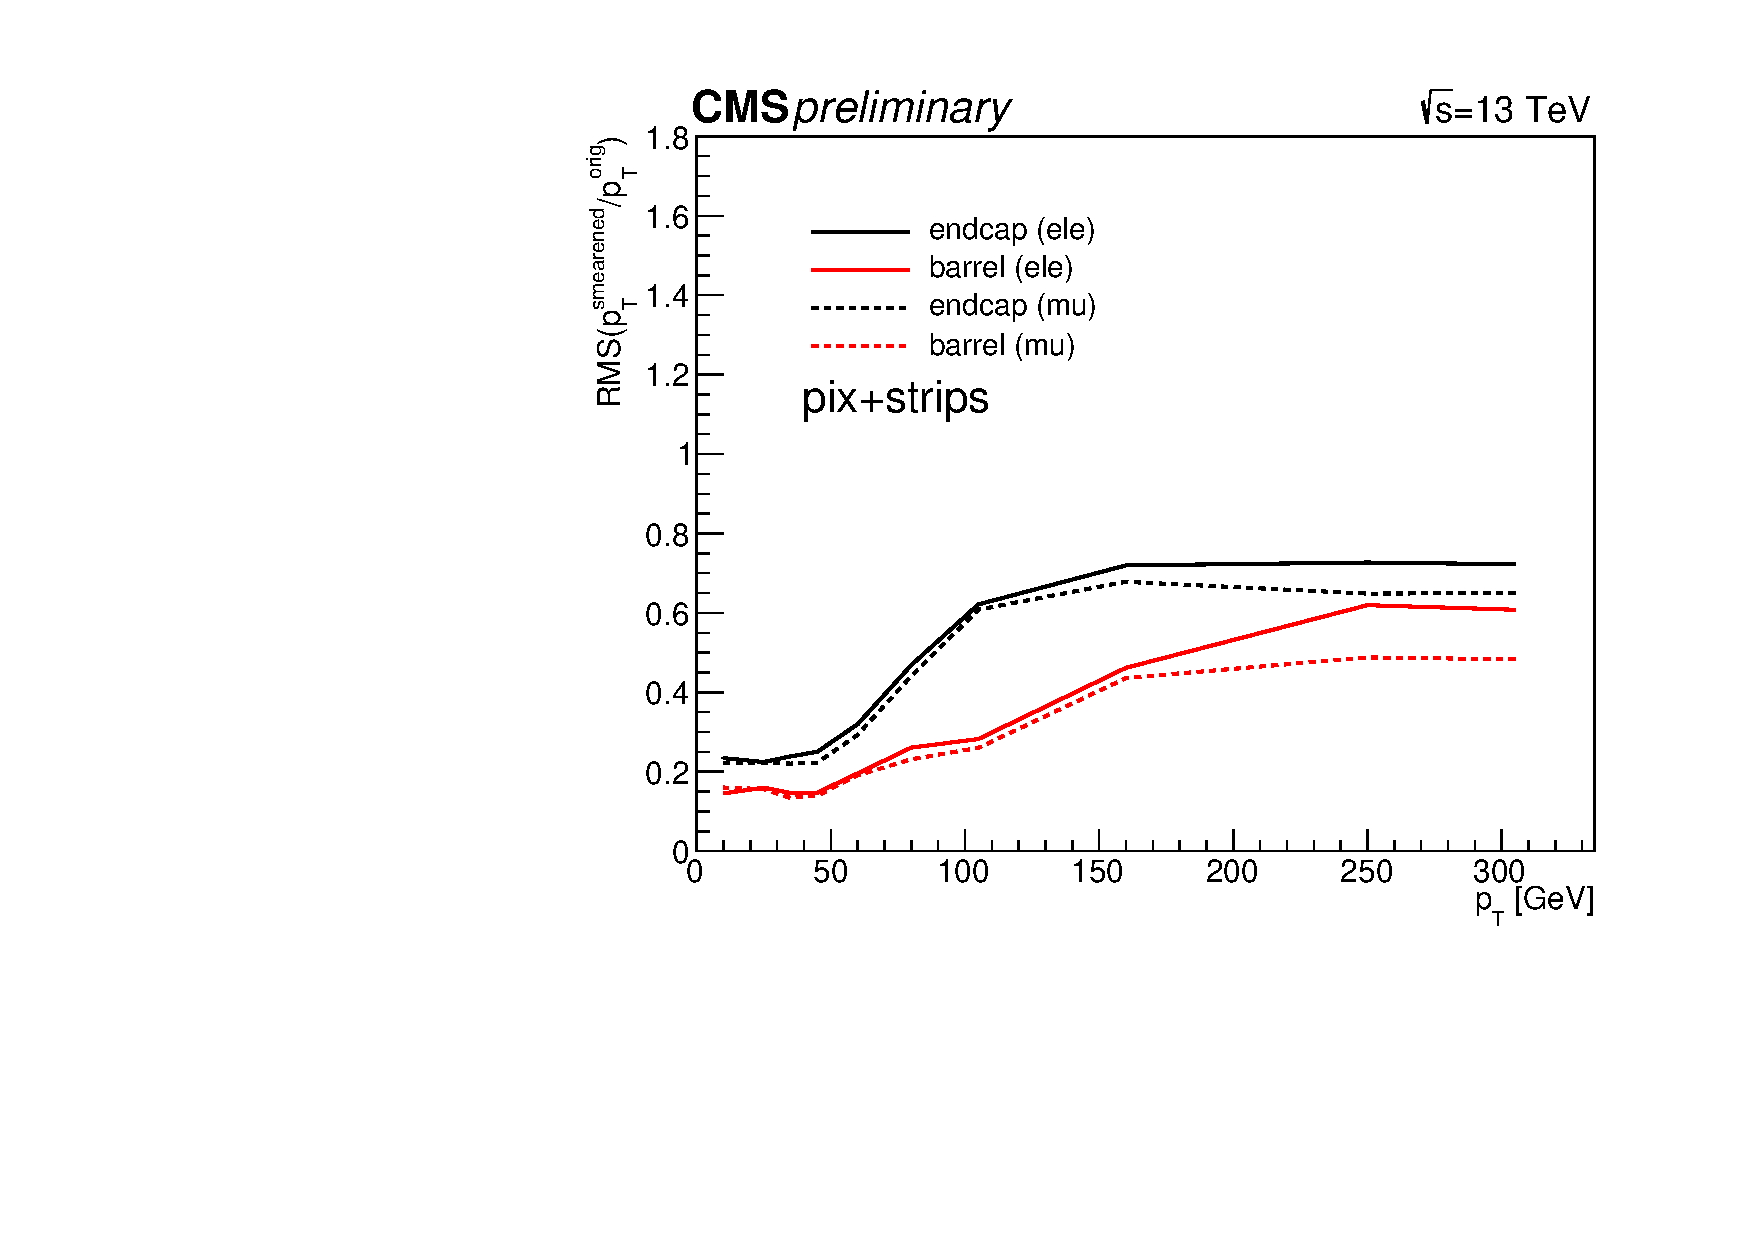
\includegraphics[width=.5\linewidth]{pdfs/24-RmsVsPt_PixAndStrips.pdf}
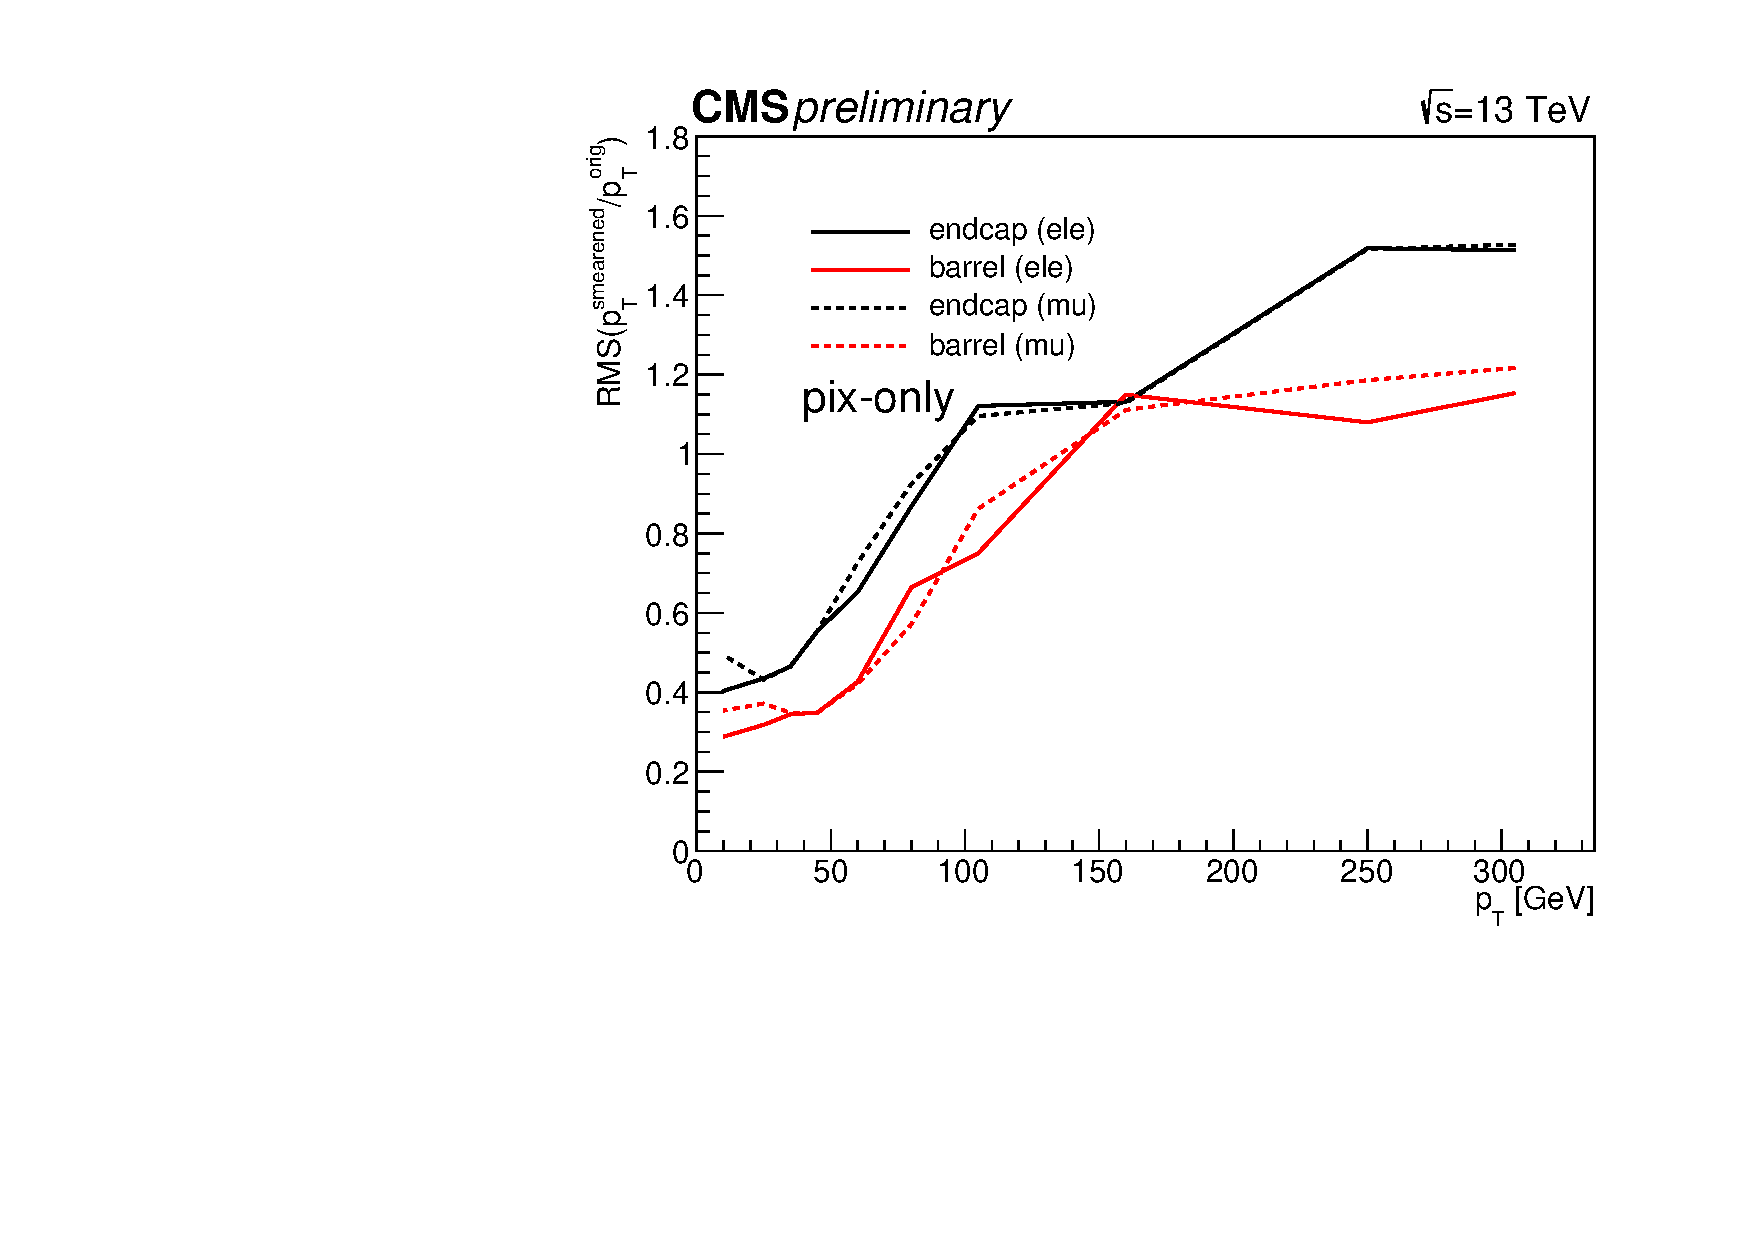
\includegraphics[width=.5\linewidth]{pdfs/25-RmsVsPt_PixOnly.pdf}
}


\frame{\frametitle{Masks}
\scriptsize
An eta/phi mask seems appropriate - veto tracks that fall within white area below, defined by bins with a normalized occupancy $>0.5*10^{-4}$ \\
\vspace{.4cm}
\centering
\begin{columns}
\column{.5\textwidth}
\centering
\scriptsize
before mask\\
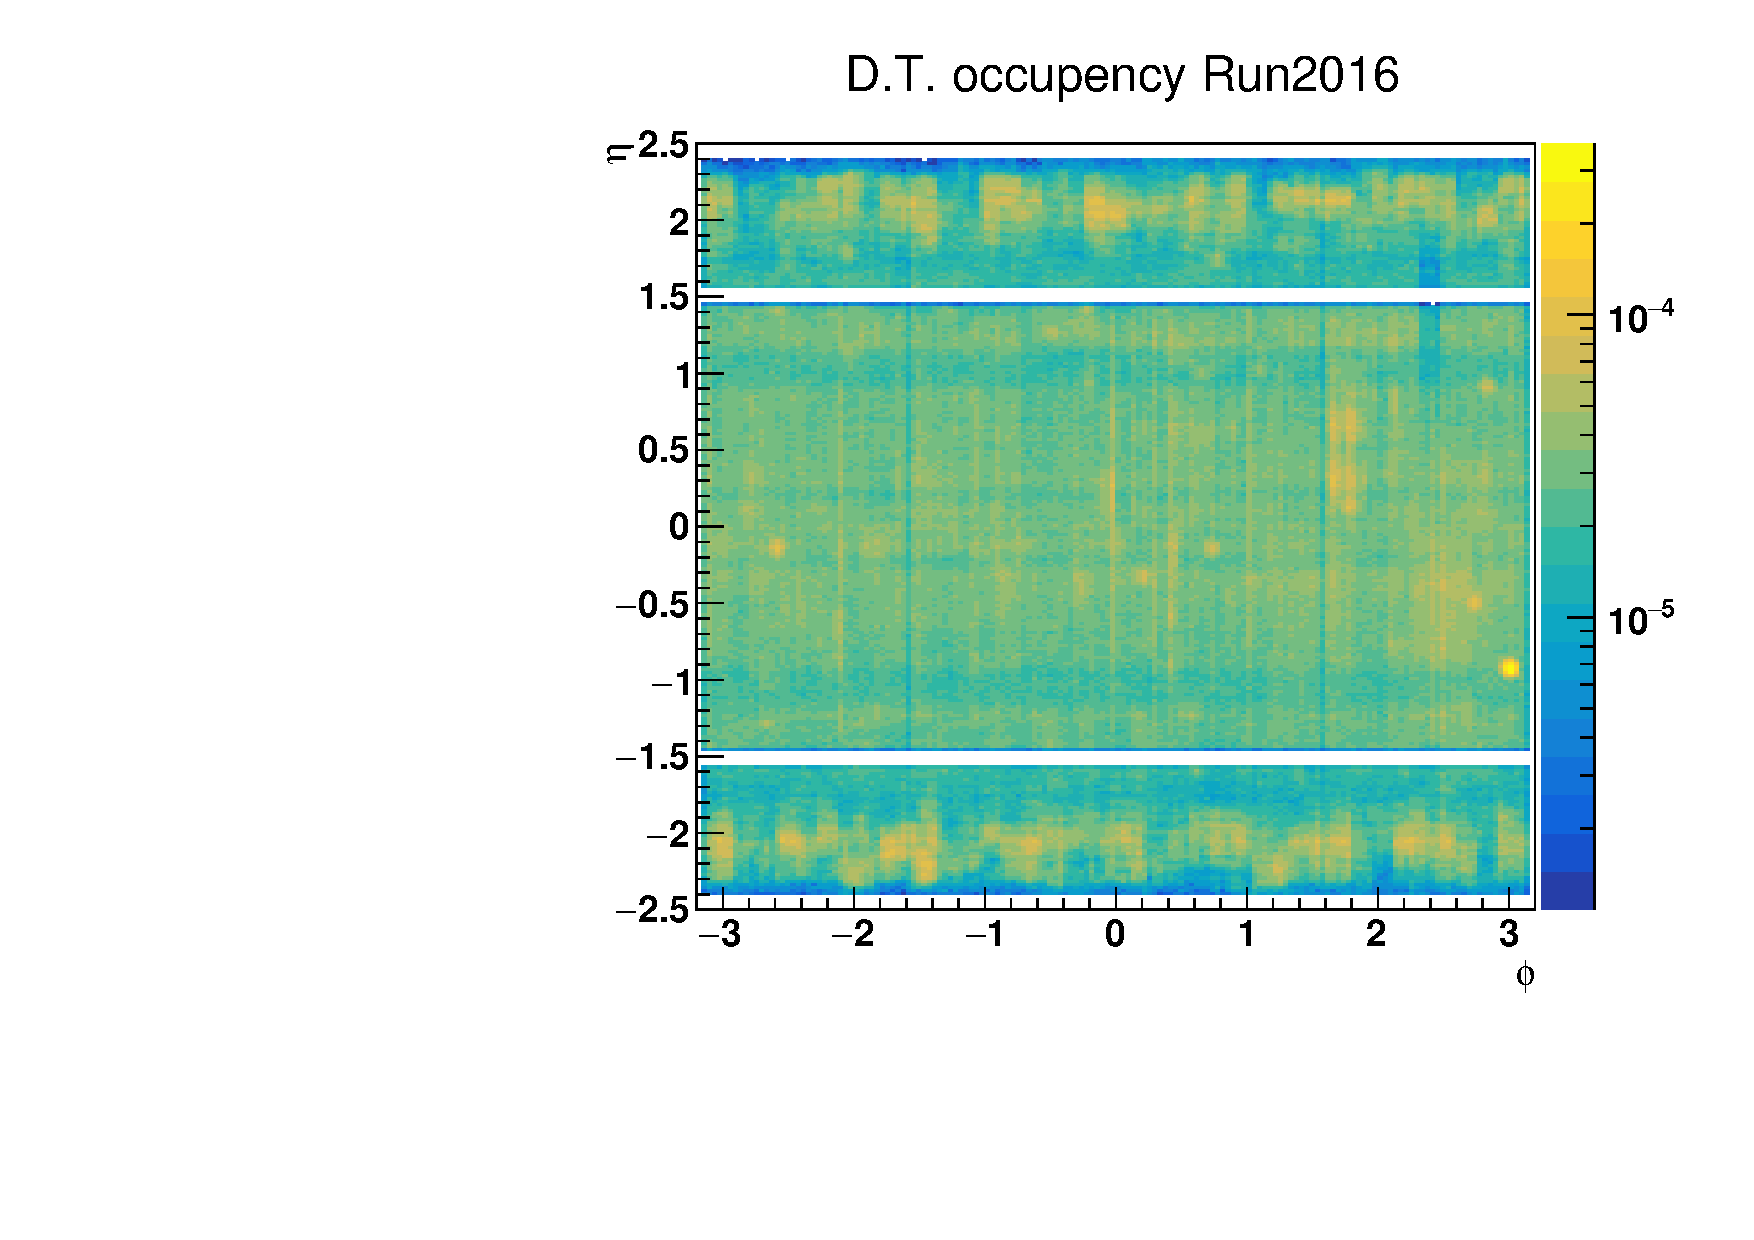
\includegraphics[width=\textwidth]{pdfs/26-hEtaVsPhiDTRun2016.pdf}
\column{.5\textwidth}
\centering
\scriptsize
after mask\\
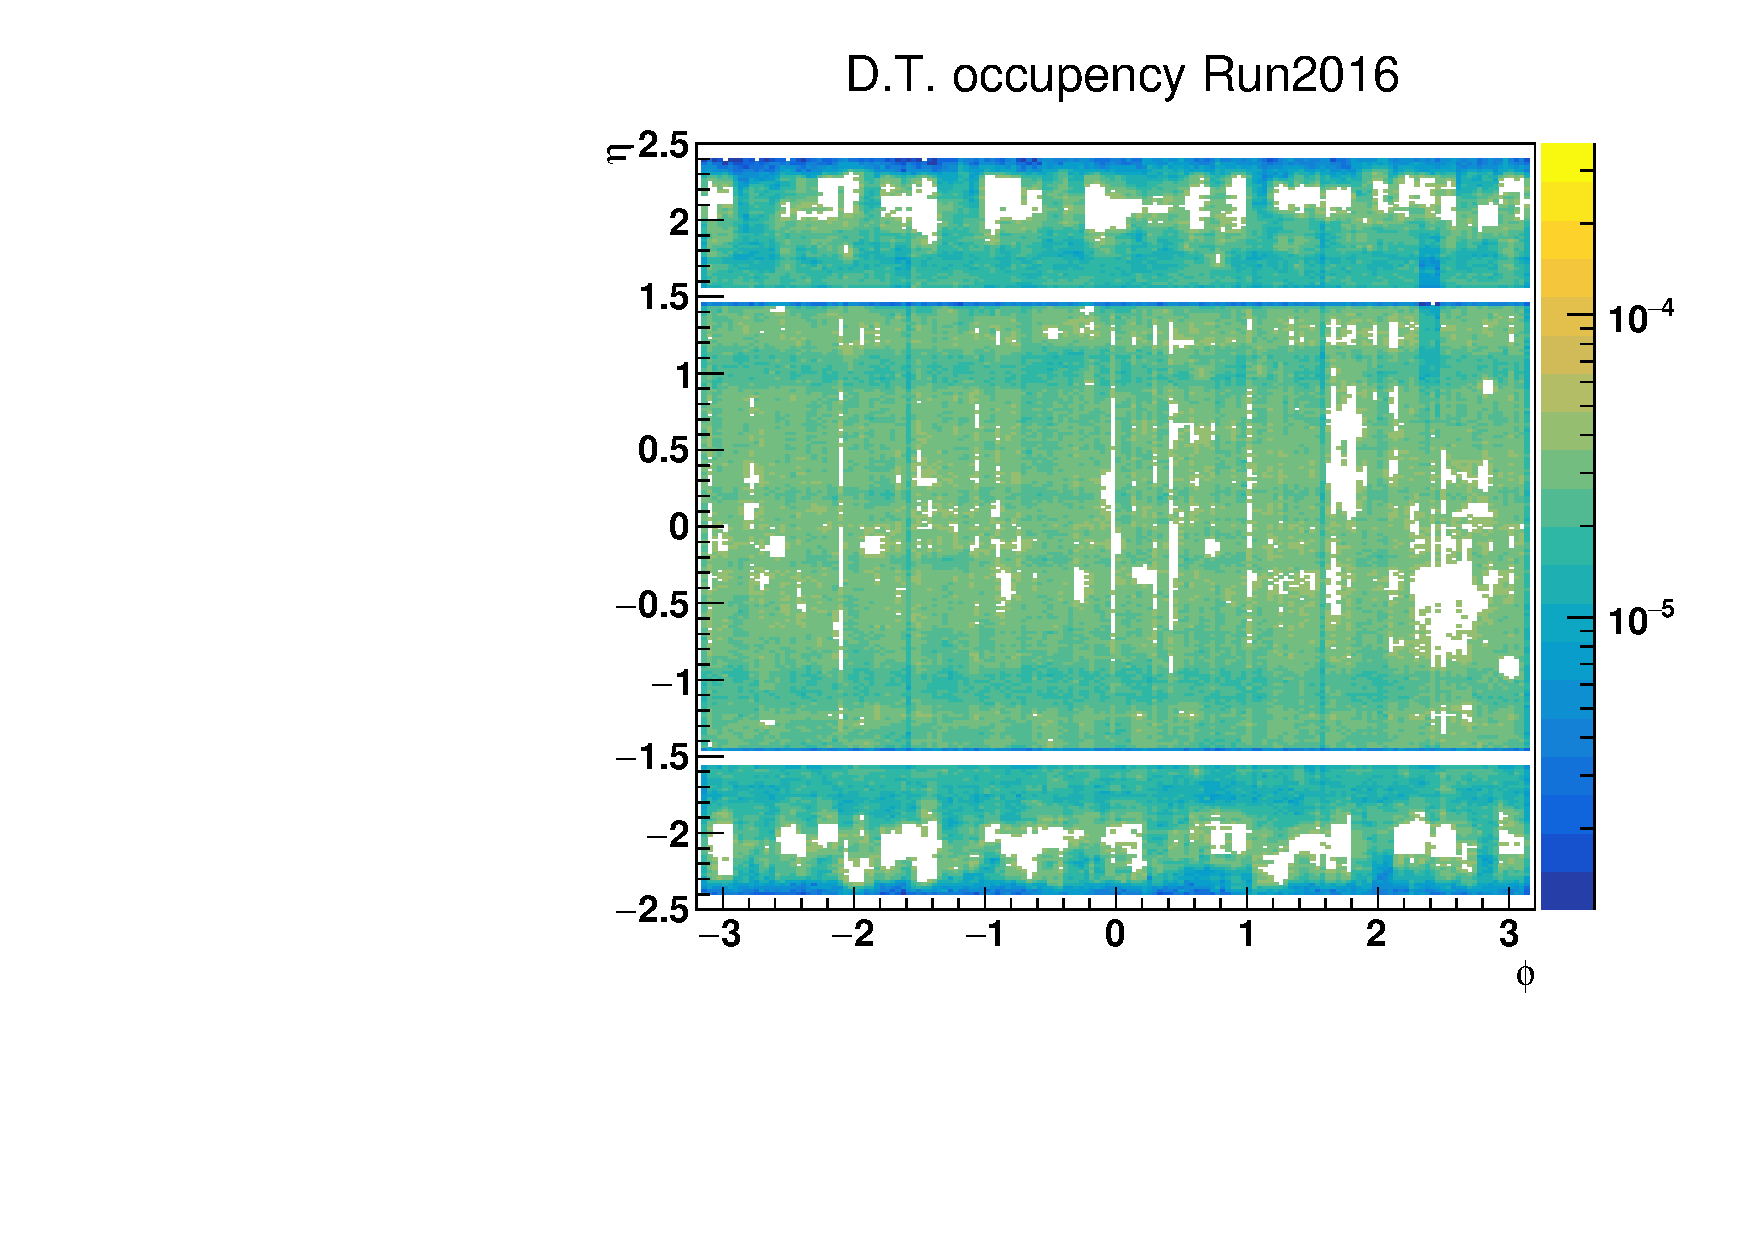
\includegraphics[width=\textwidth]{pdfs/27-hEtaVsPhiDT_maskedRun2016.pdf}
\end{columns}
\scriptsize
mask histograms are made available in Mattermost in rootfiles
}


\frame{\frametitle{Masks 2016B}
\scriptsize
Explore run-dependent masks, defined by bins with a normalized occupancy $>0.5*10^{-4}$ \\
\vspace{.4cm}
\centering
\begin{columns}
\column{.5\textwidth}
\centering
\scriptsize
before mask\\
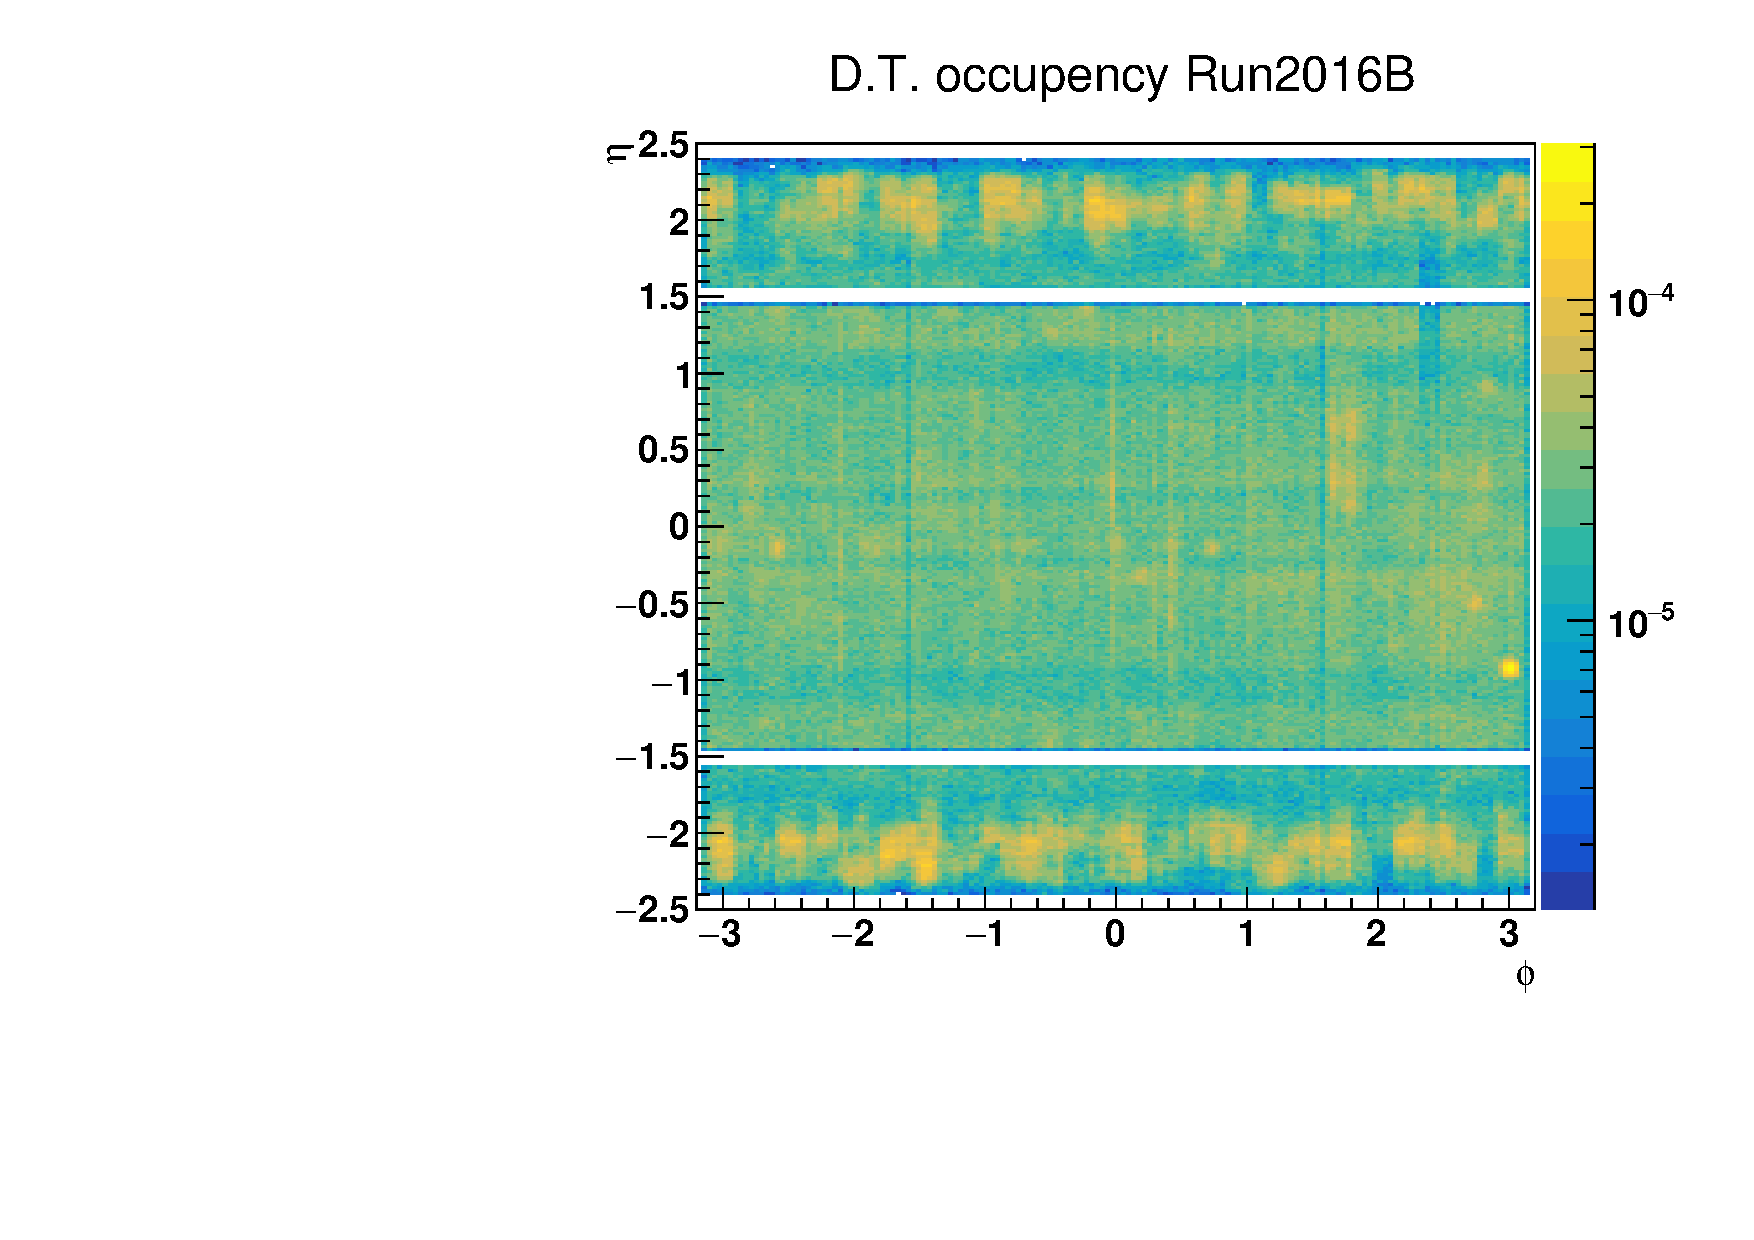
\includegraphics[width=\textwidth]{pdfs/28-hEtaVsPhiDTRun2016B.pdf}
\column{.5\textwidth}
\centering
\scriptsize
after mask\\
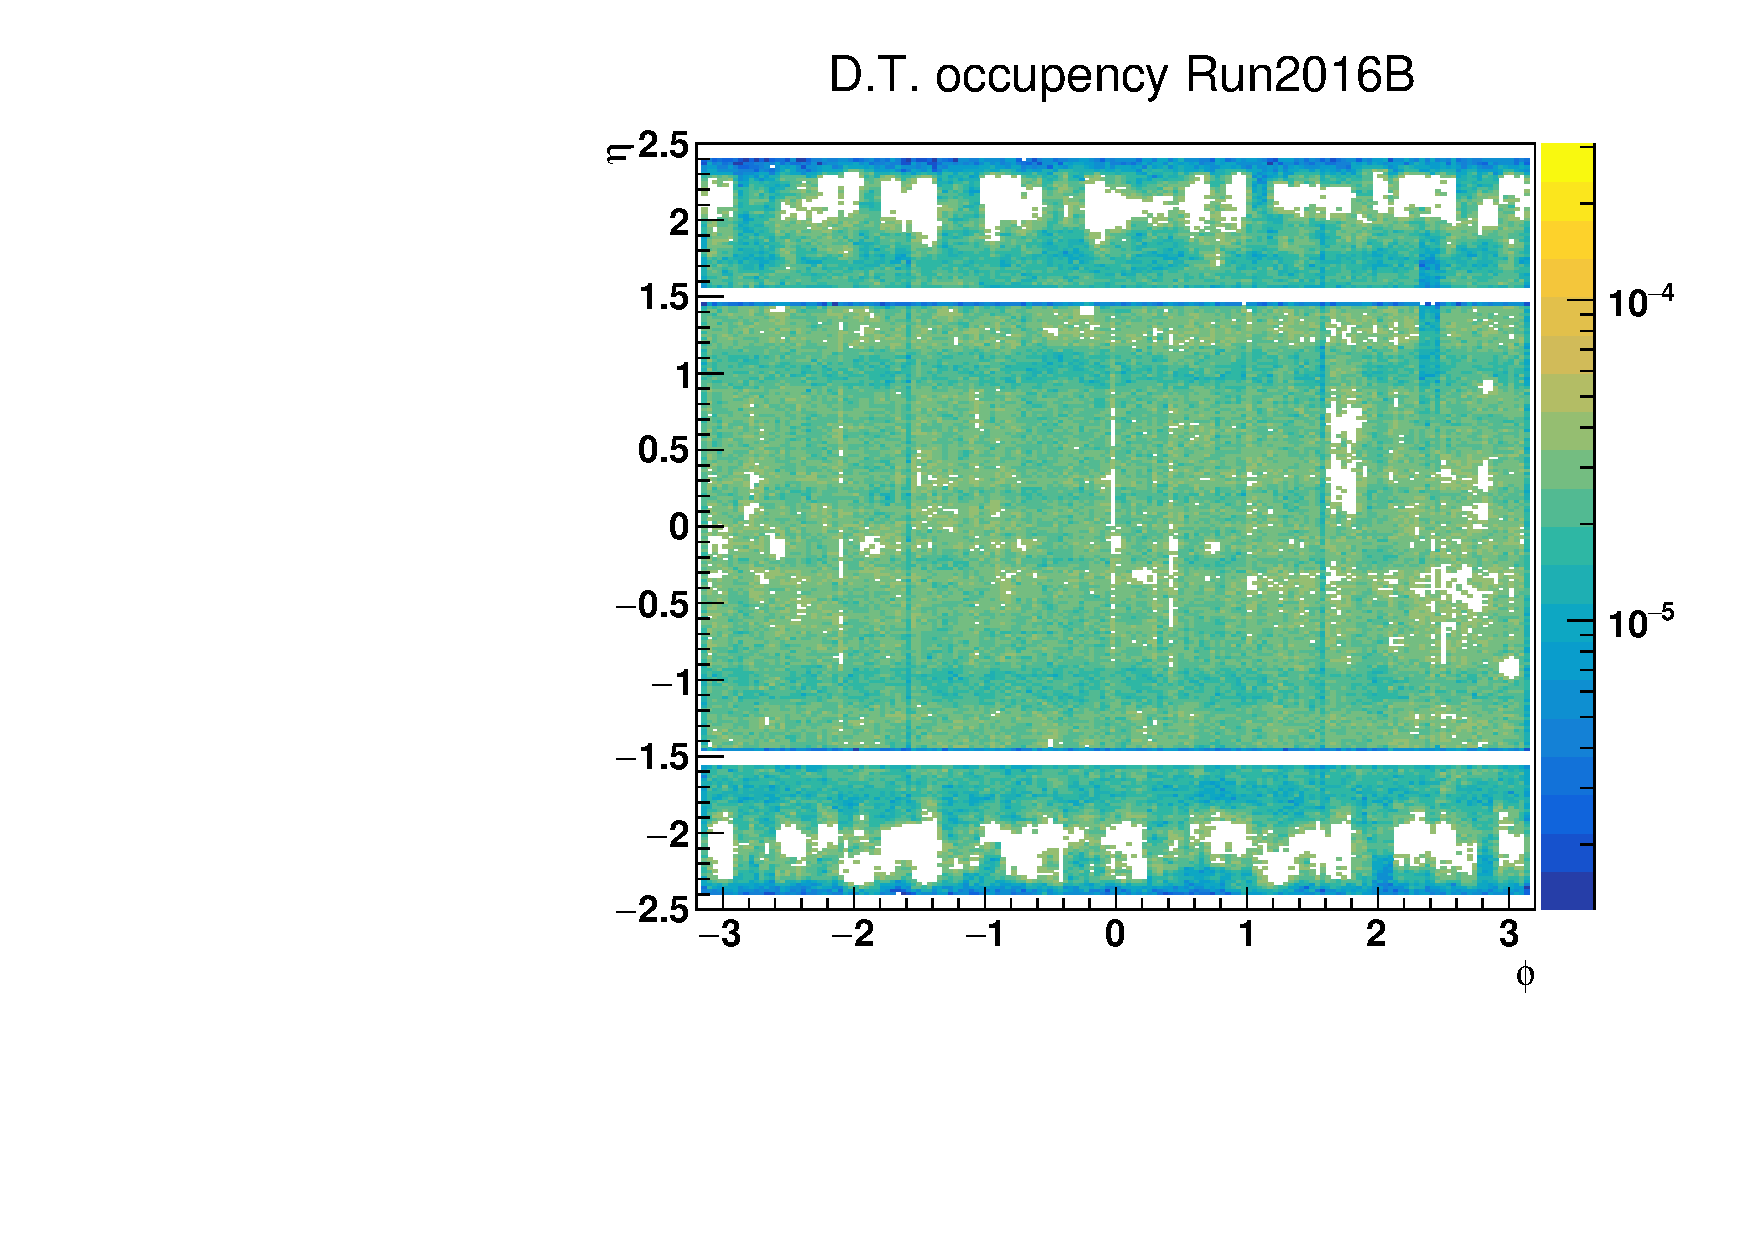
\includegraphics[width=\textwidth]{pdfs/29-hEtaVsPhiDT_maskedRun2016B.pdf}
\end{columns}
\scriptsize
mask histograms are made available in Mattermost in rootfiles
}

\frame{\frametitle{Masks 2016D}
\scriptsize
Explore run-dependent masks, defined by bins with a normalized occupancy $>0.5*10^{-4}$ \\
\vspace{.4cm}
\centering
\begin{columns}
\column{.5\textwidth}
\centering
\scriptsize
before mask\\
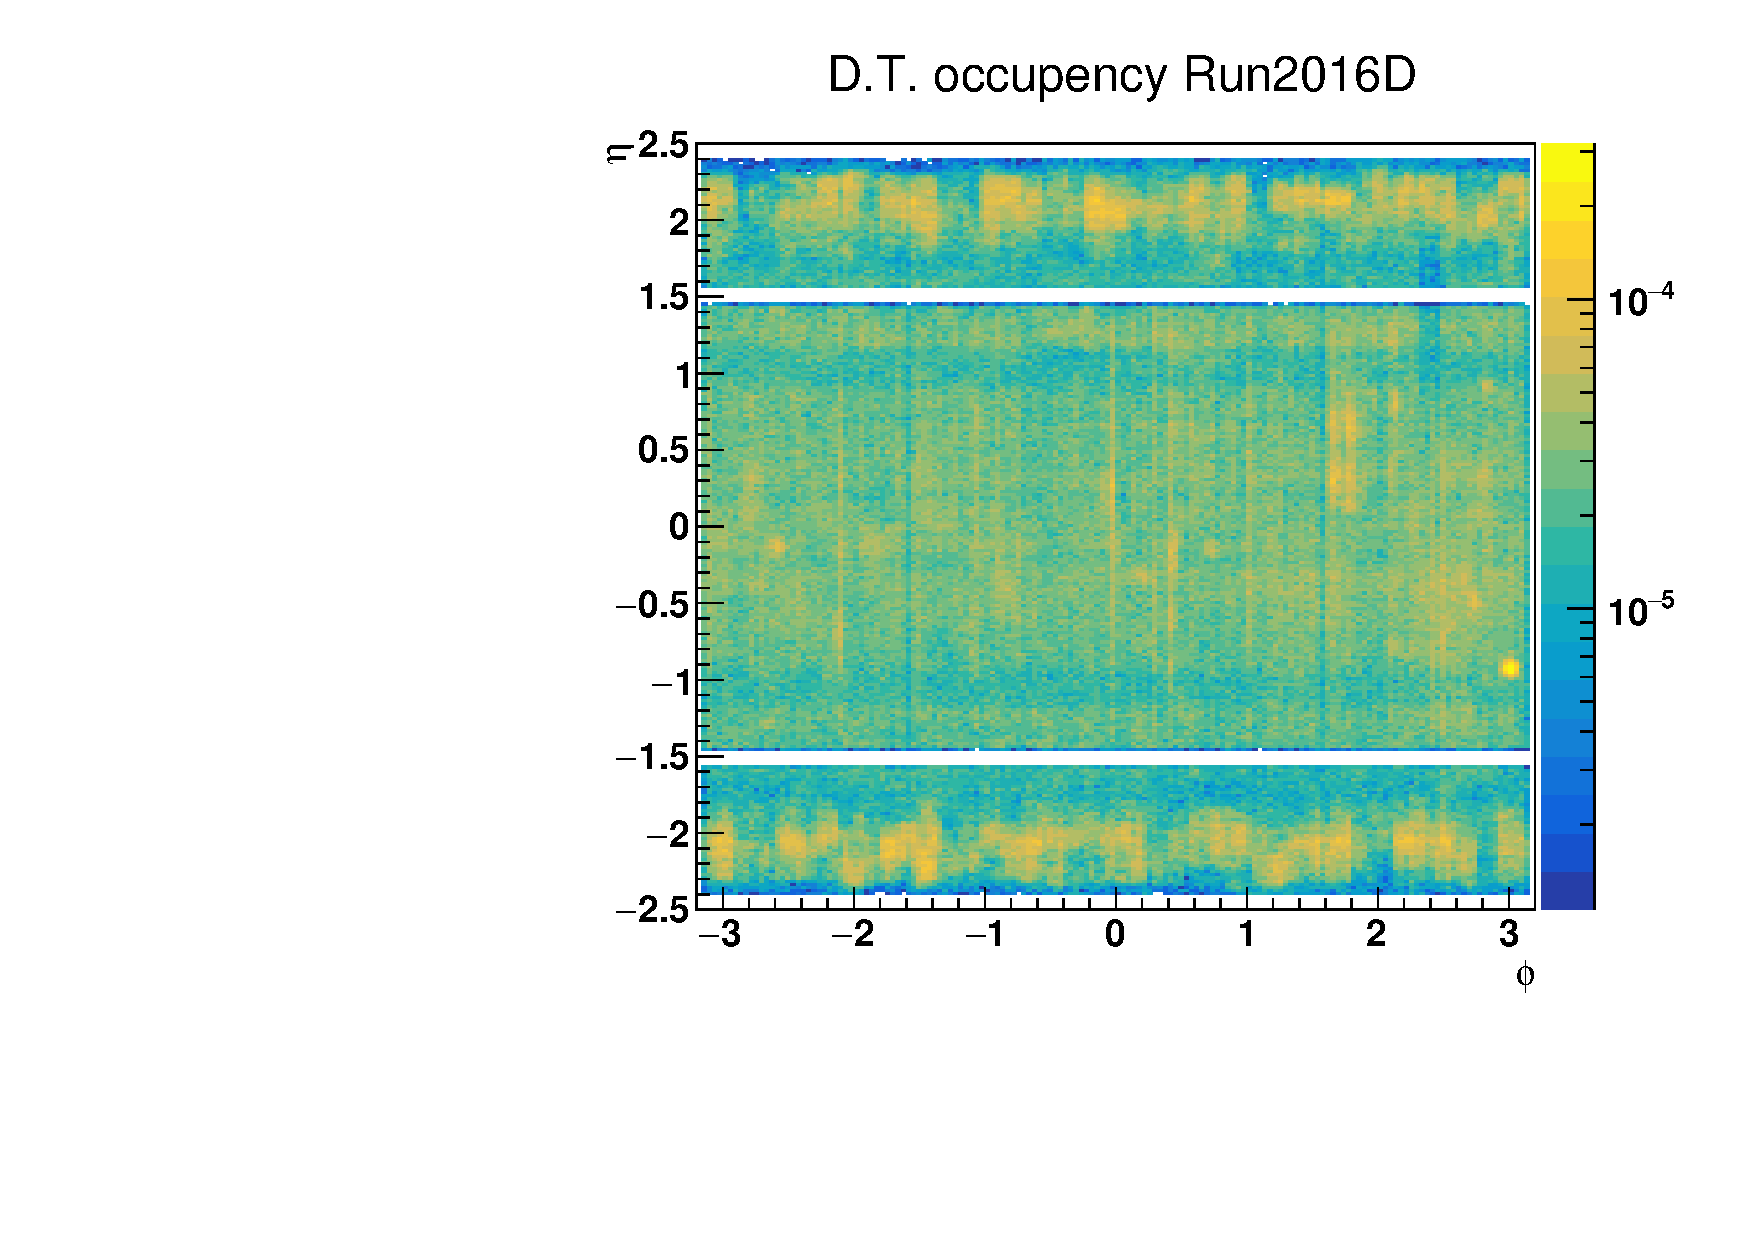
\includegraphics[width=\textwidth]{pdfs/30-hEtaVsPhiDTRun2016D.pdf}
\column{.5\textwidth}
\centering
\scriptsize
after mask\\
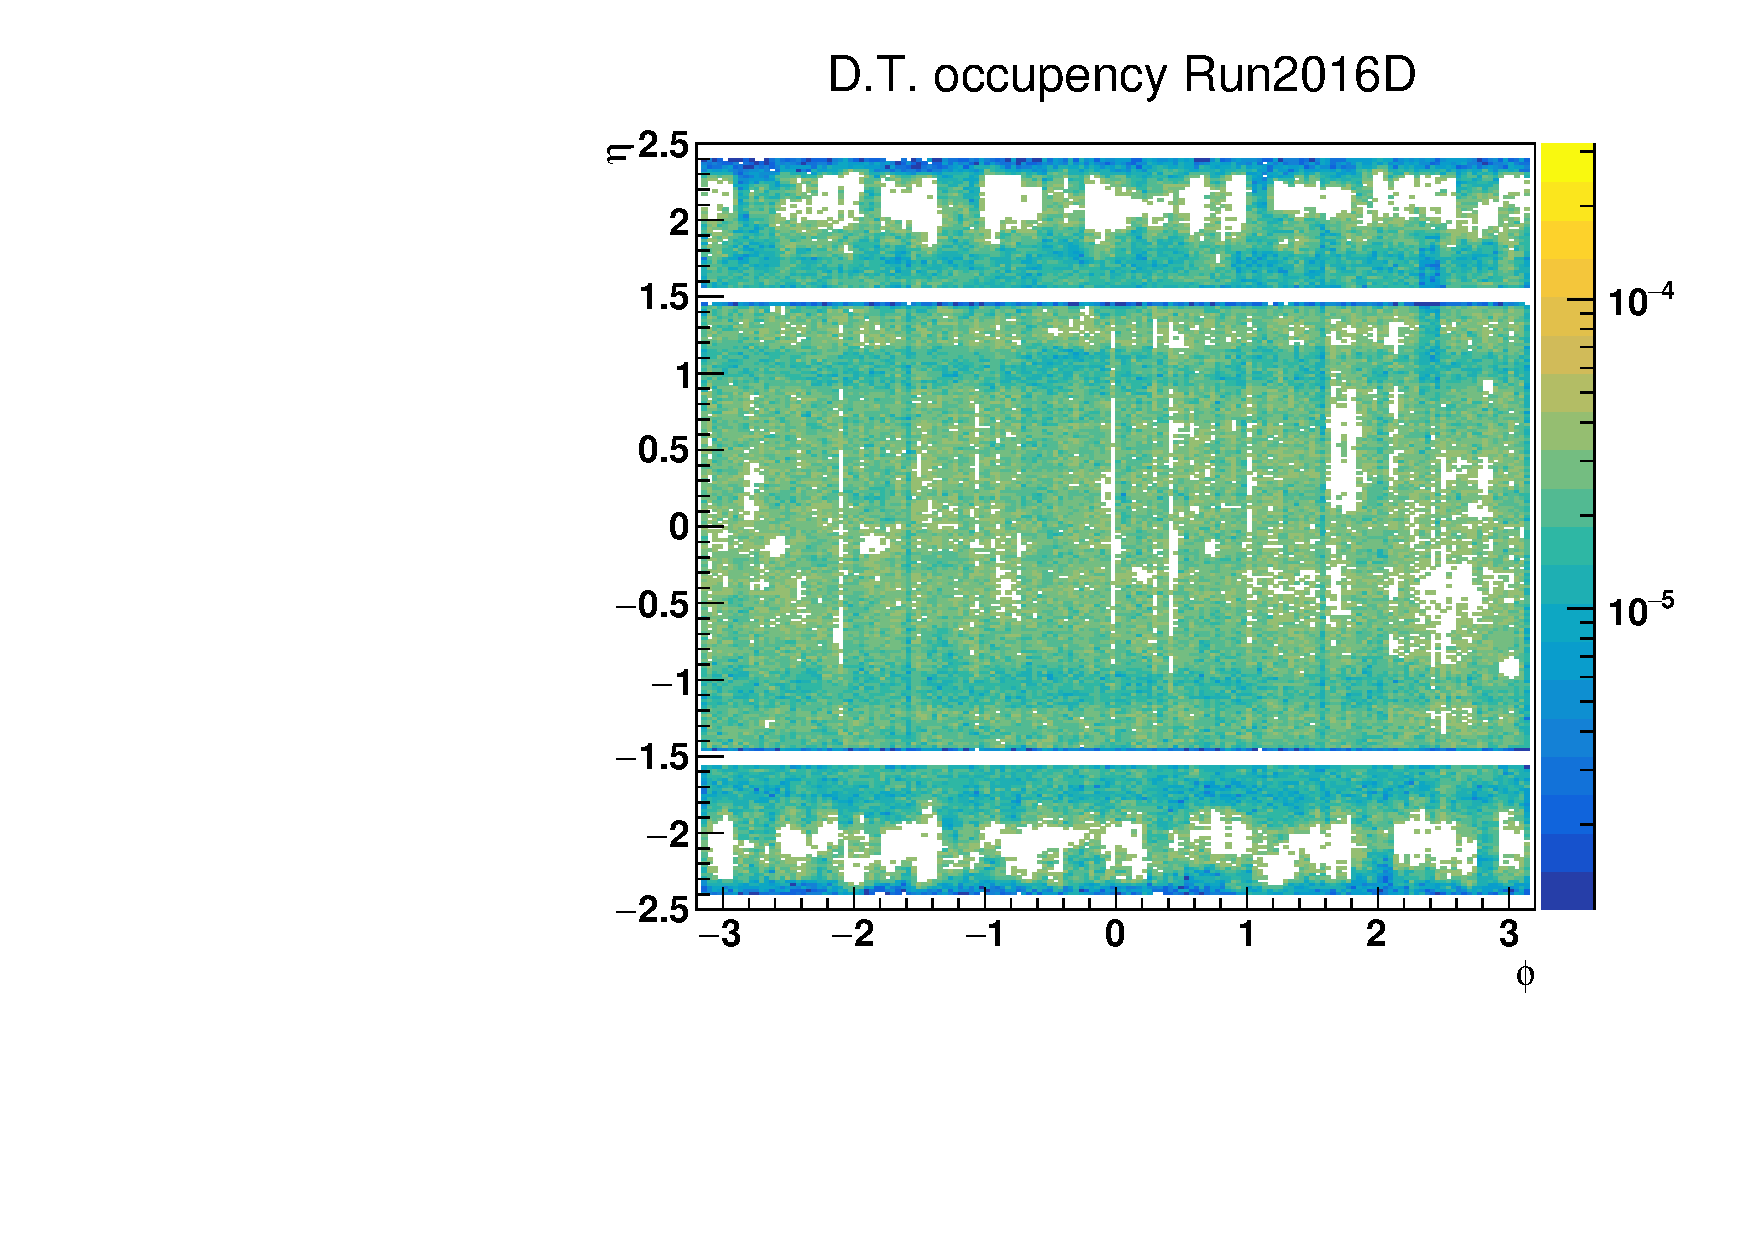
\includegraphics[width=\textwidth]{pdfs/31-hEtaVsPhiDT_maskedRun2016D.pdf}
\end{columns}
\scriptsize
mask histograms are made available in Mattermost in rootfiles
}

\frame{\frametitle{Masks 2016G}
\scriptsize
Explore run-dependent masks, defined by bins with a normalized occupancy $>0.5*10^{-4}$ \\
\vspace{.4cm}
\centering
\begin{columns}
\column{.5\textwidth}
\centering
\scriptsize
before mask\\
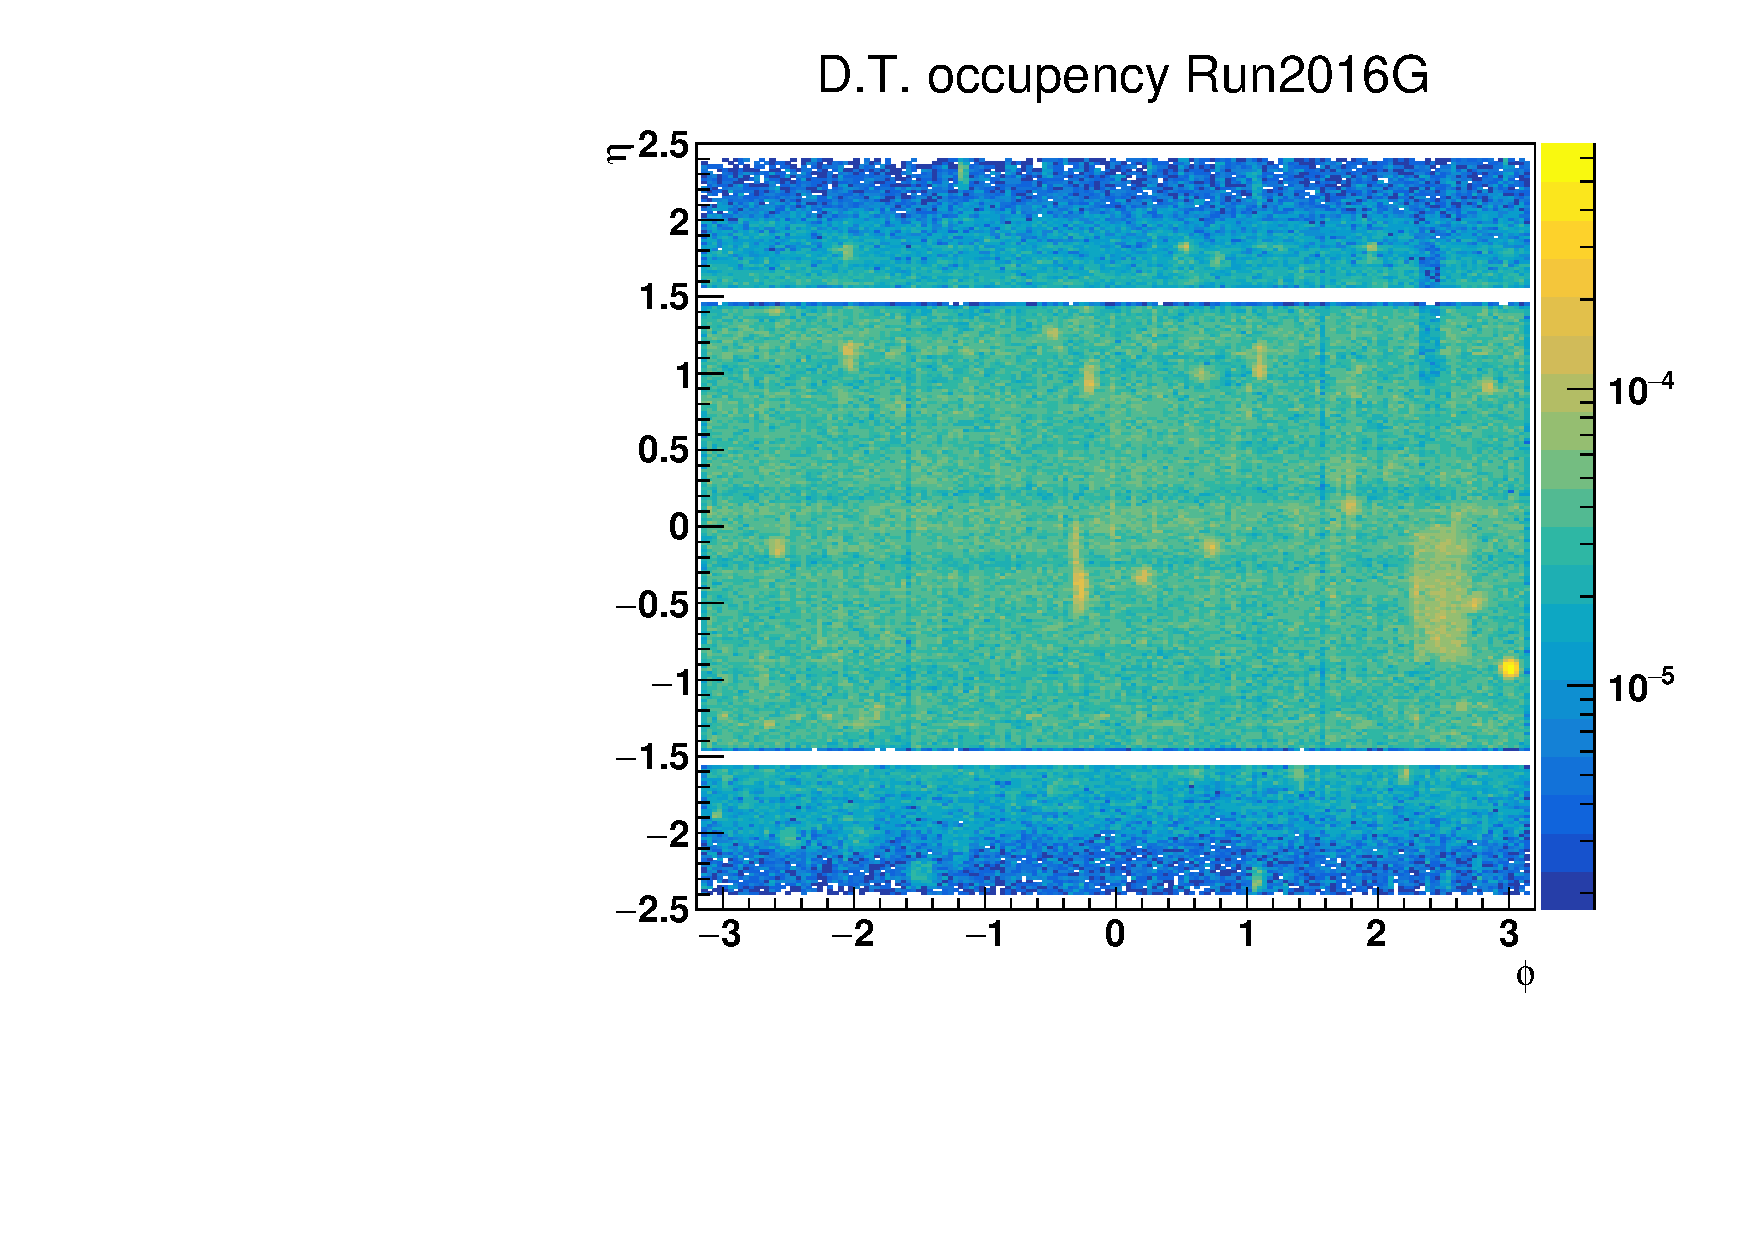
\includegraphics[width=\textwidth]{pdfs/32-hEtaVsPhiDTRun2016G.pdf}
\column{.5\textwidth}
\centering
\scriptsize
after mask\\
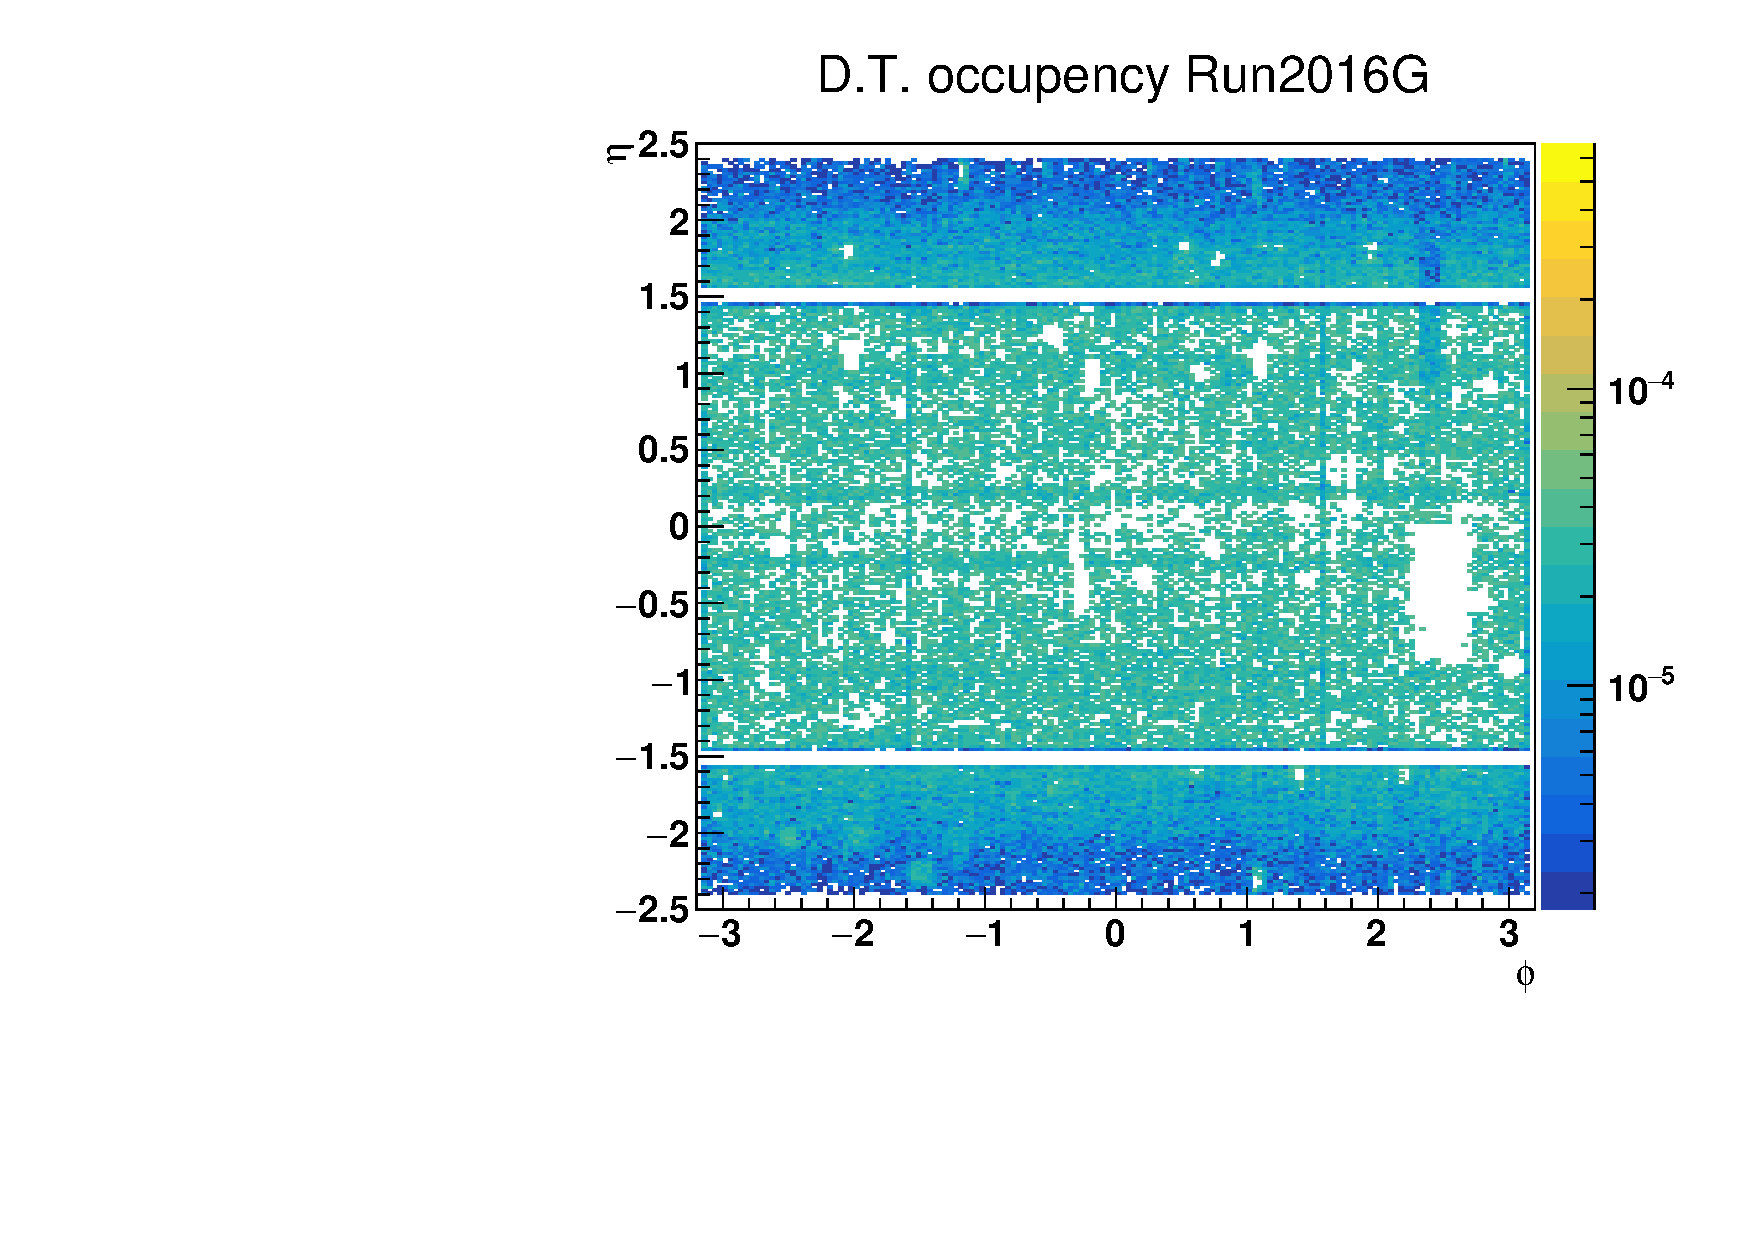
\includegraphics[width=\textwidth]{pdfs/33-hEtaVsPhiDT_maskedRun2016G.pdf}
\end{columns}
}

\frame{\frametitle{Model T1btbLL (requested)}
\begin{center}
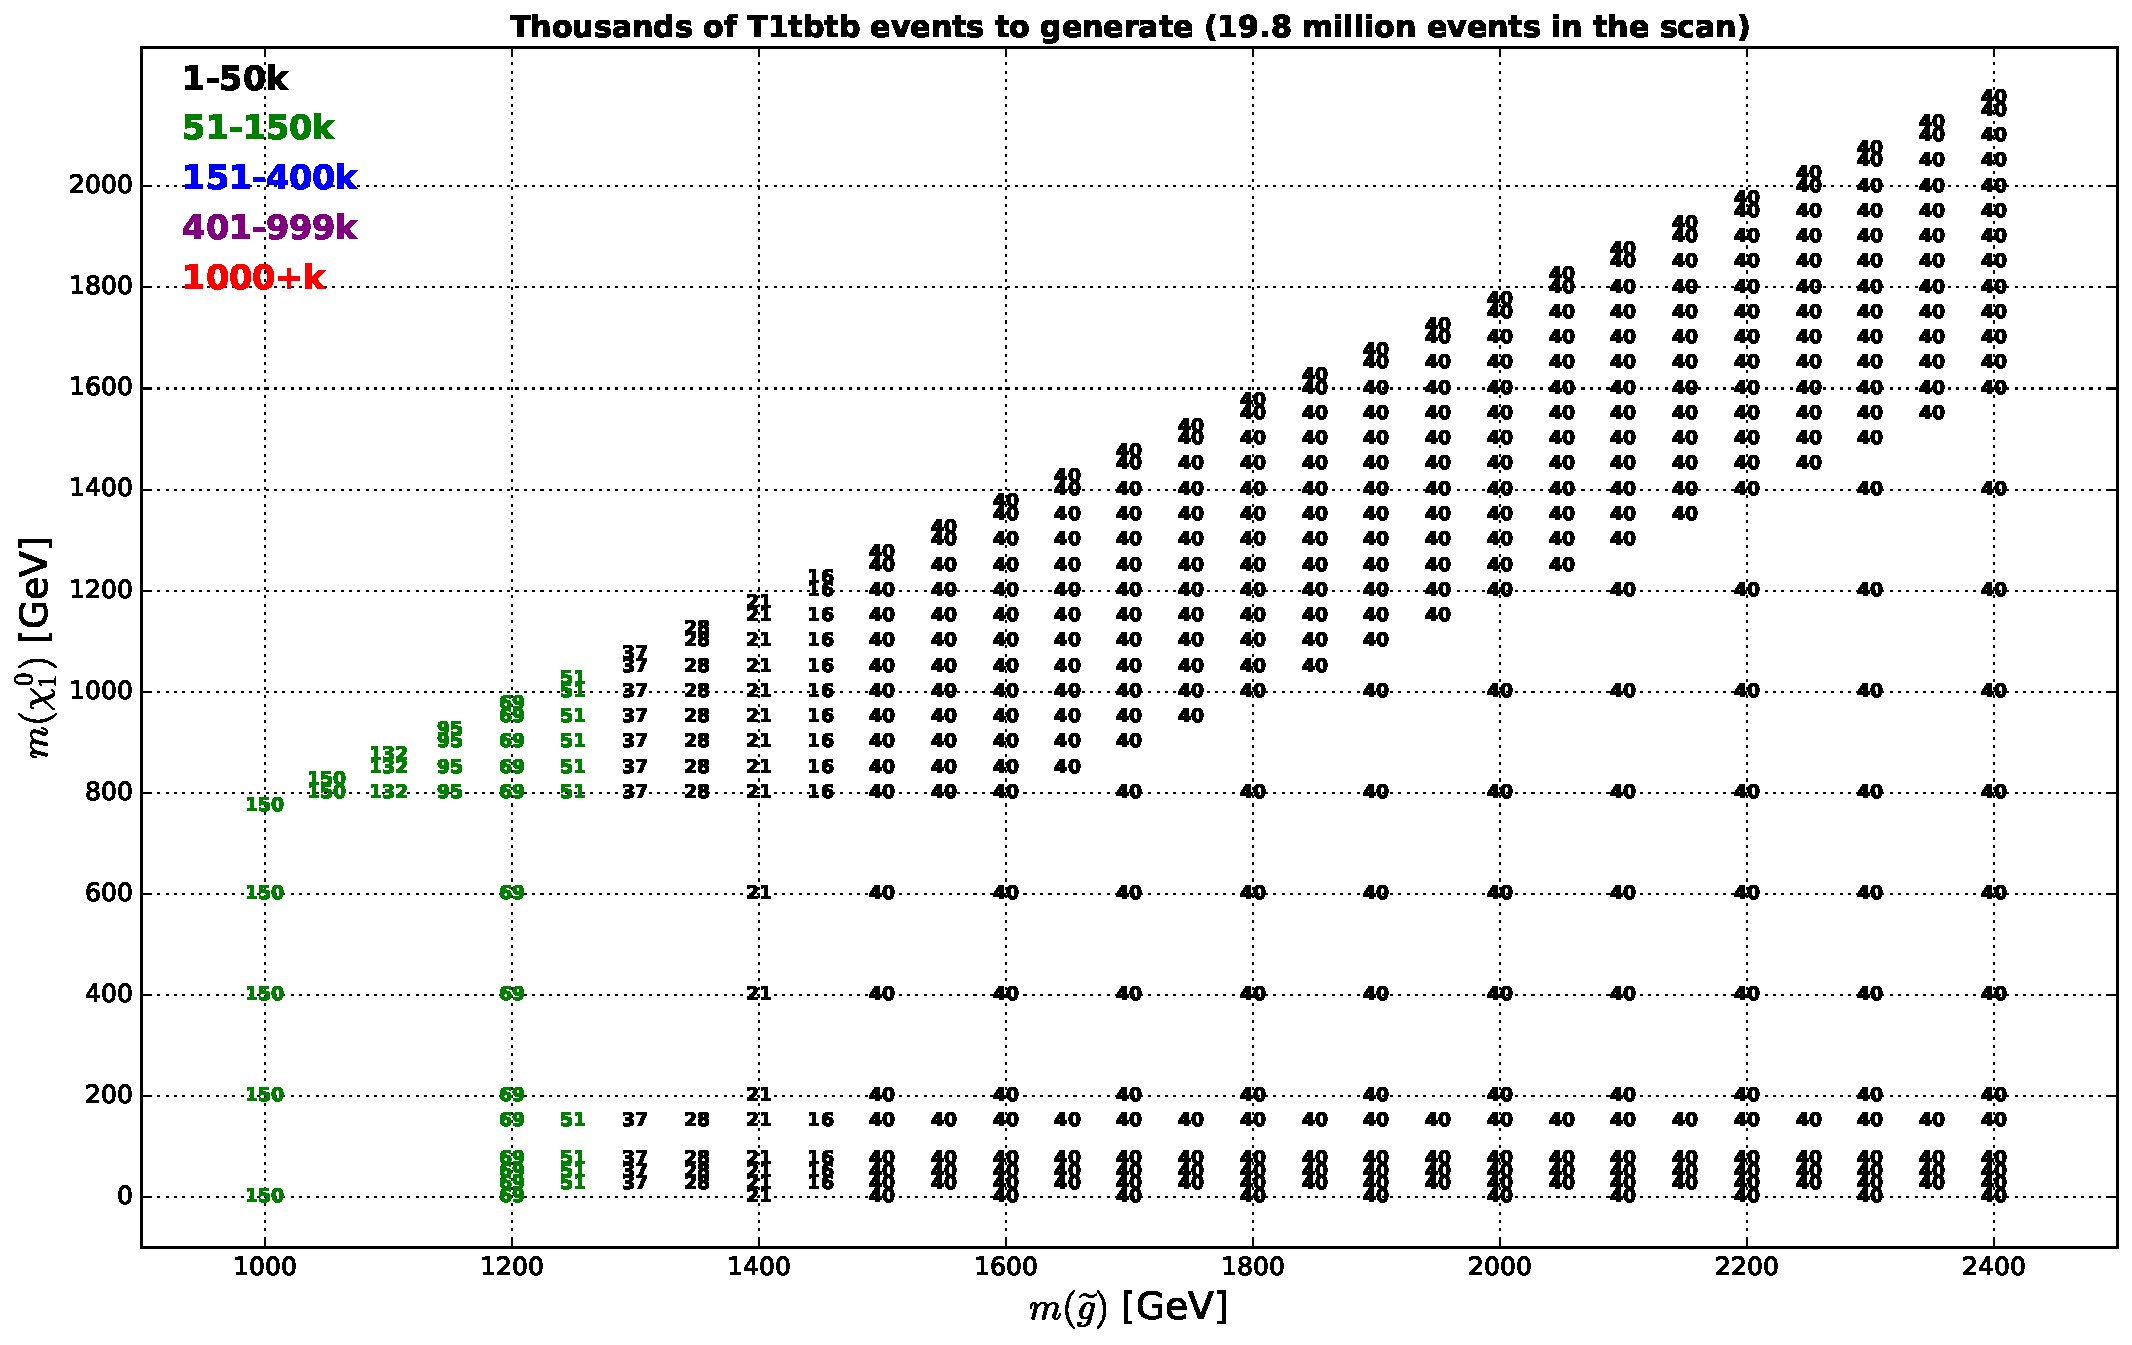
\includegraphics[width=\linewidth]{pdfs/34-T1tbtb_events.pdf}
\end{center}
}



\frame{\frametitle{Electron background closure}
\begin{flushleft}
``n-1" post-baseline plots using W+jets and $t\bar{t}$-jets
\end{flushleft}
\vspace{-.1cm}
\centering
\begin{columns}
\column{.4\linewidth}
\centering
\scriptsize
MHT\\
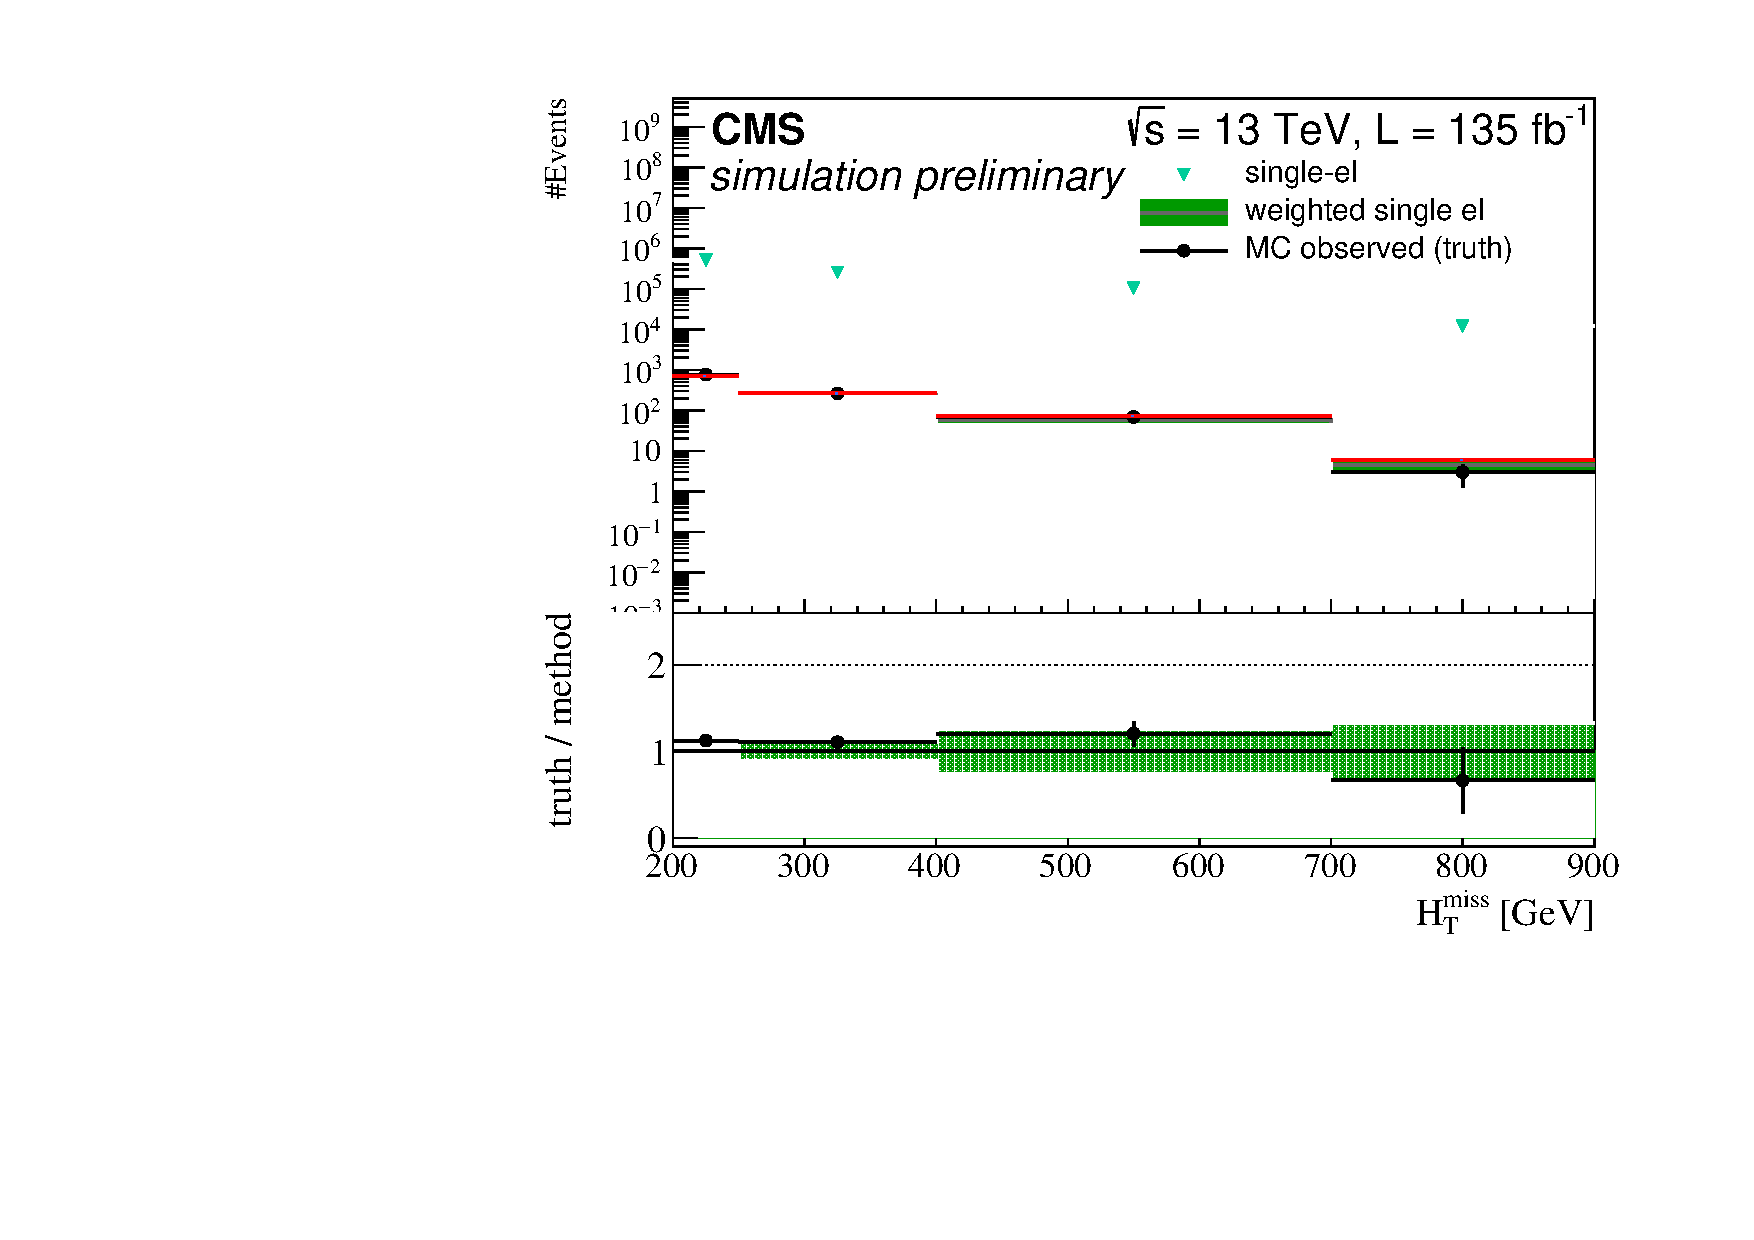
\includegraphics[width=0.8\linewidth]{pdfs/35-ElBaselineMht.pdf}\\
\scriptsize
n(jets)\\
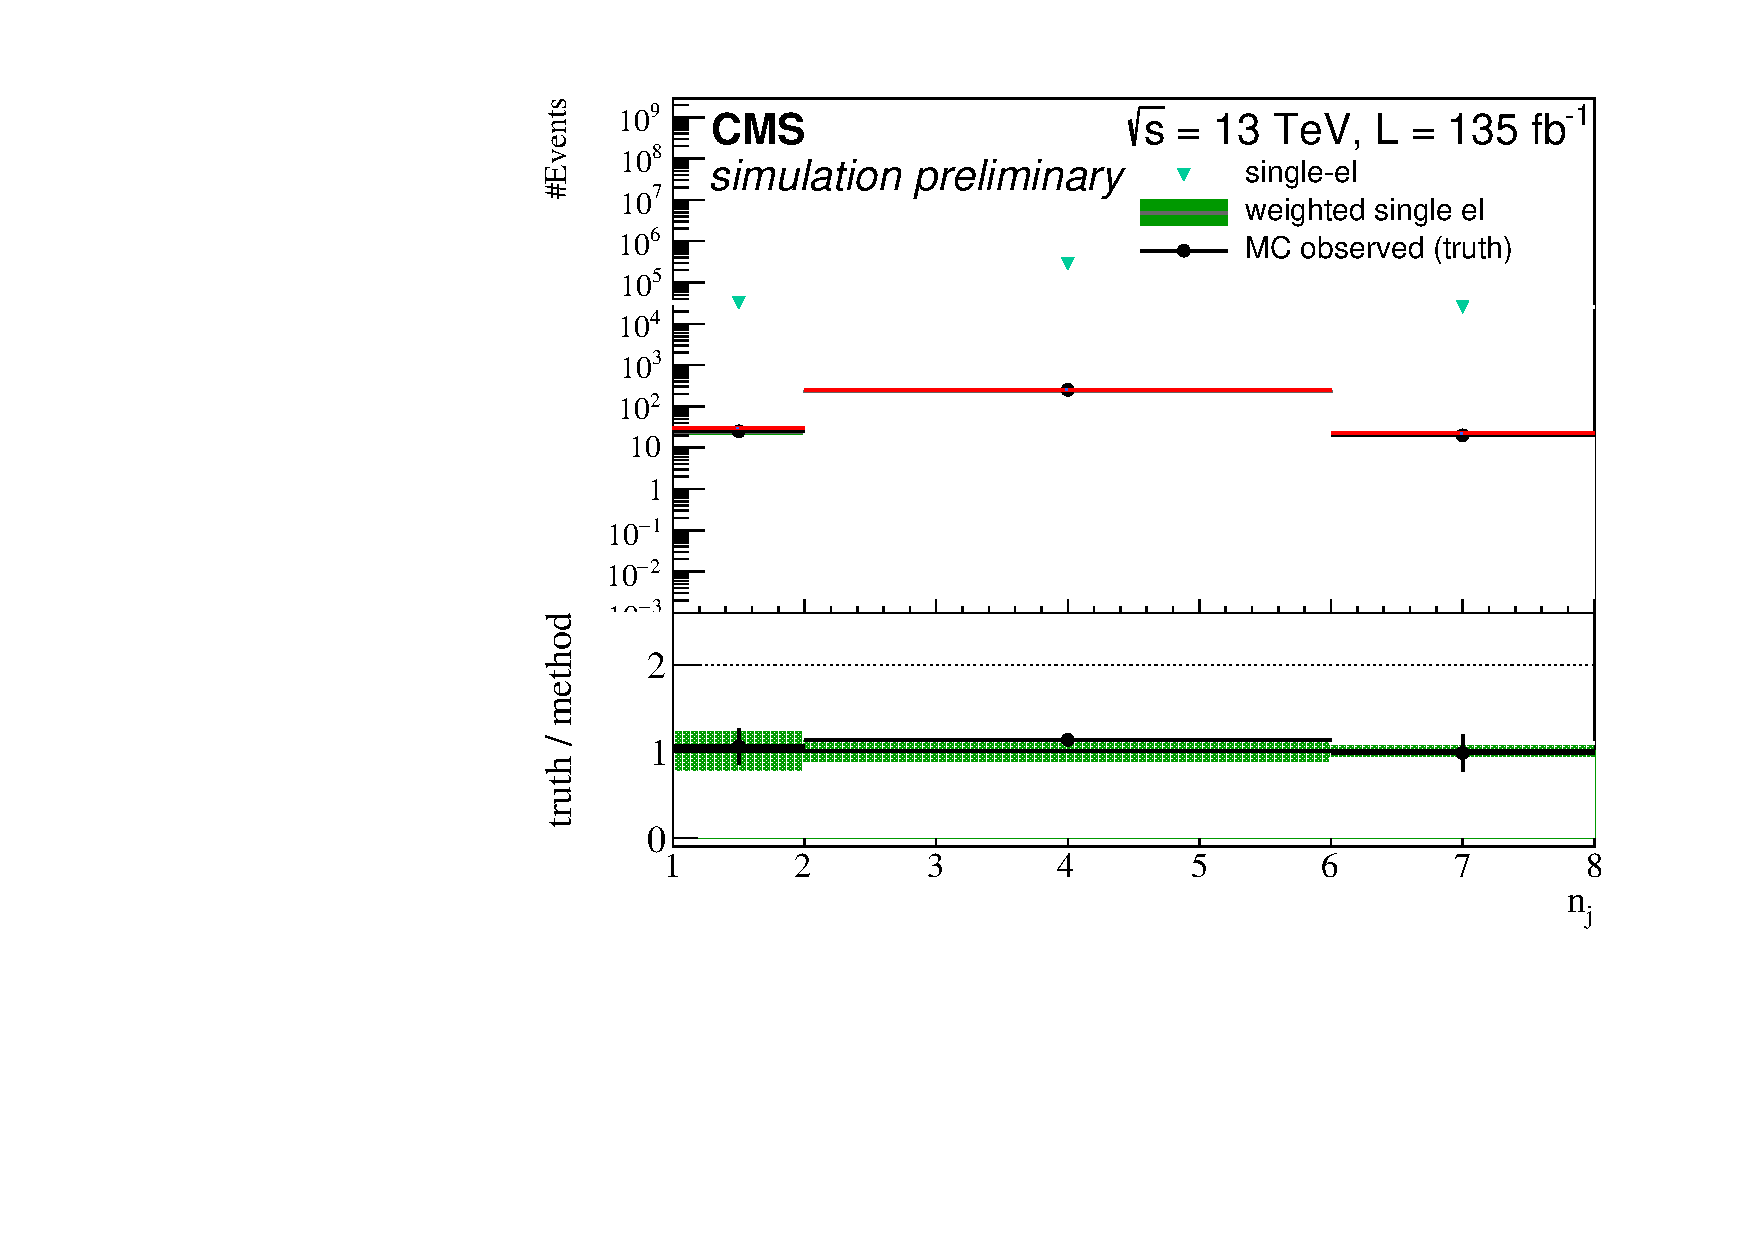
\includegraphics[width=0.8\linewidth]{pdfs/36-ElBaselineNJets.pdf}
\column{.4\linewidth}
\centering
\scriptsize
min($\Delta\phi$(jets, MHT))\\
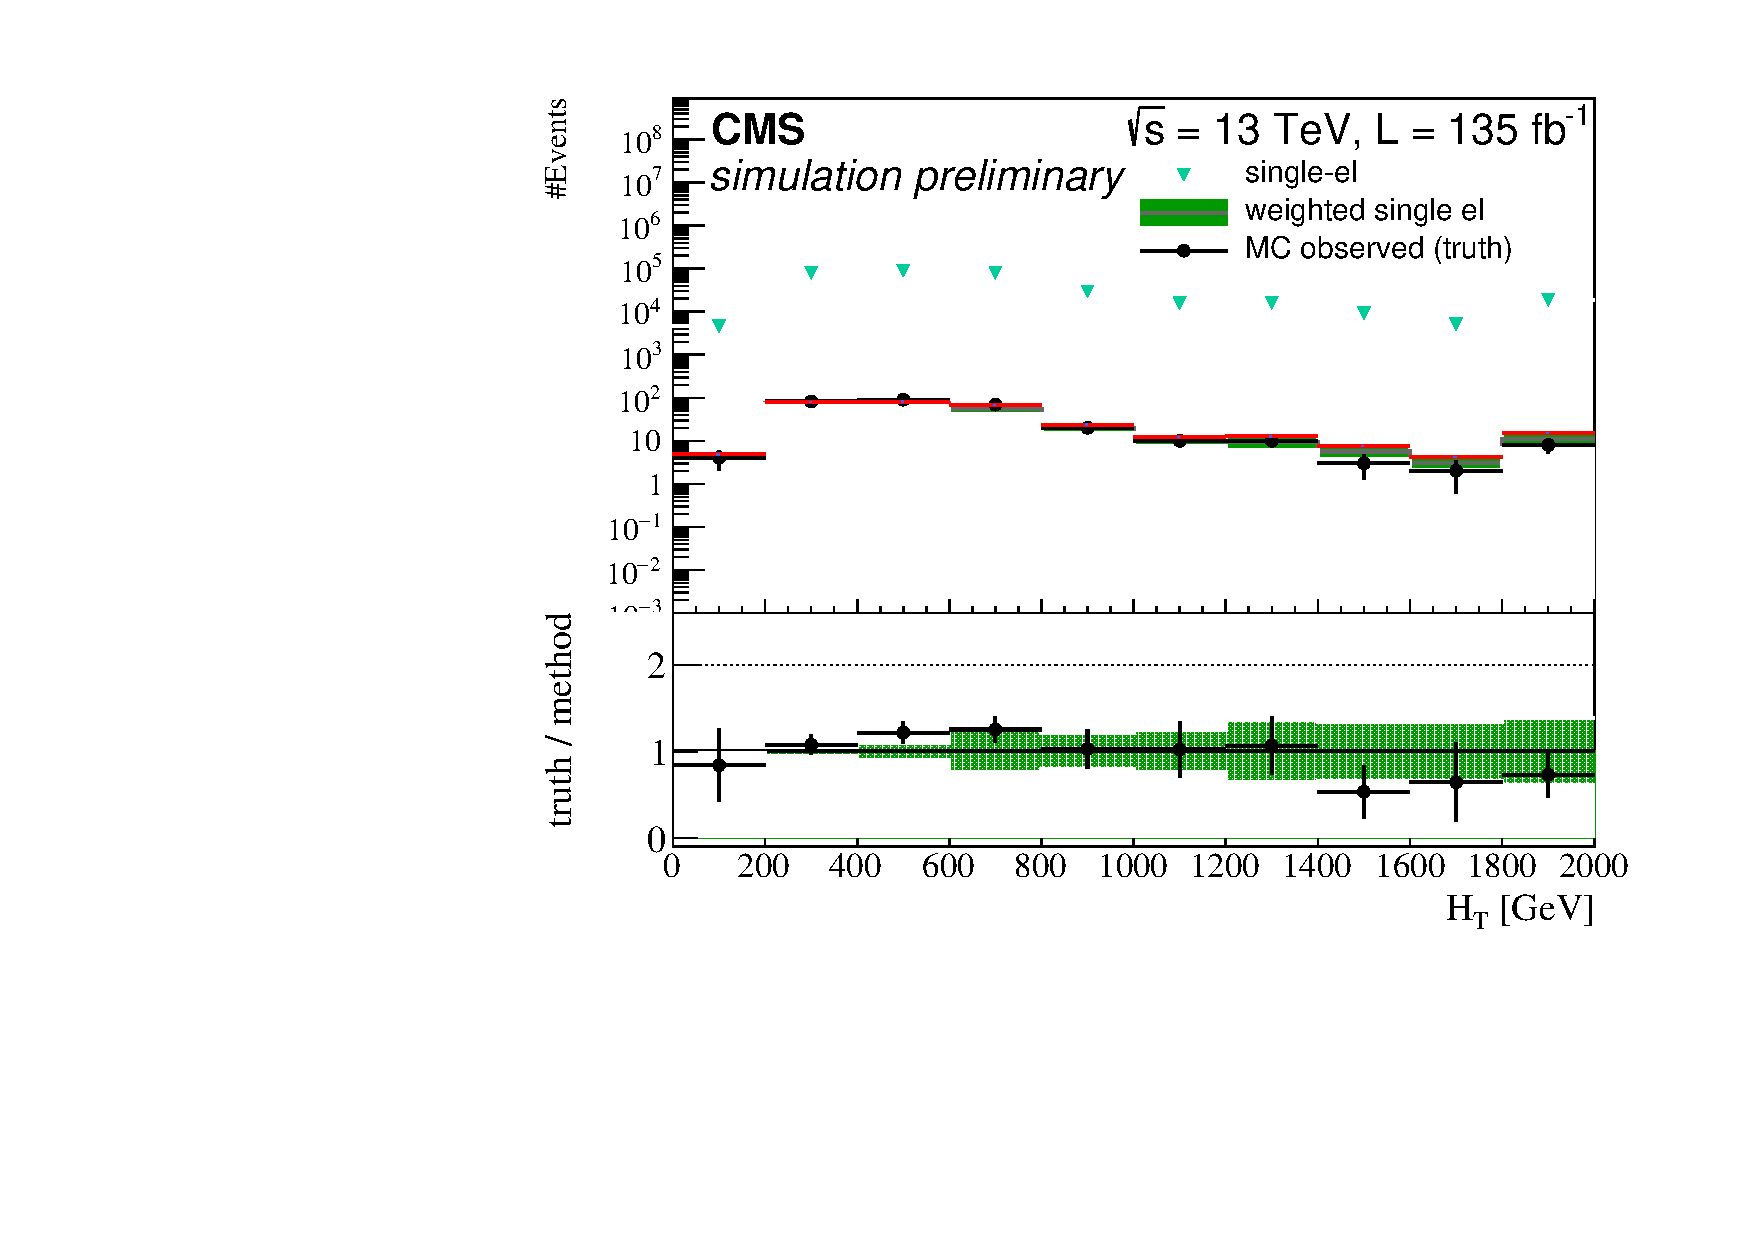
\includegraphics[width=0.8\linewidth]{pdfs/37-ElBaselineHt.pdf}\\
\scriptsize
n(b-tags)\\
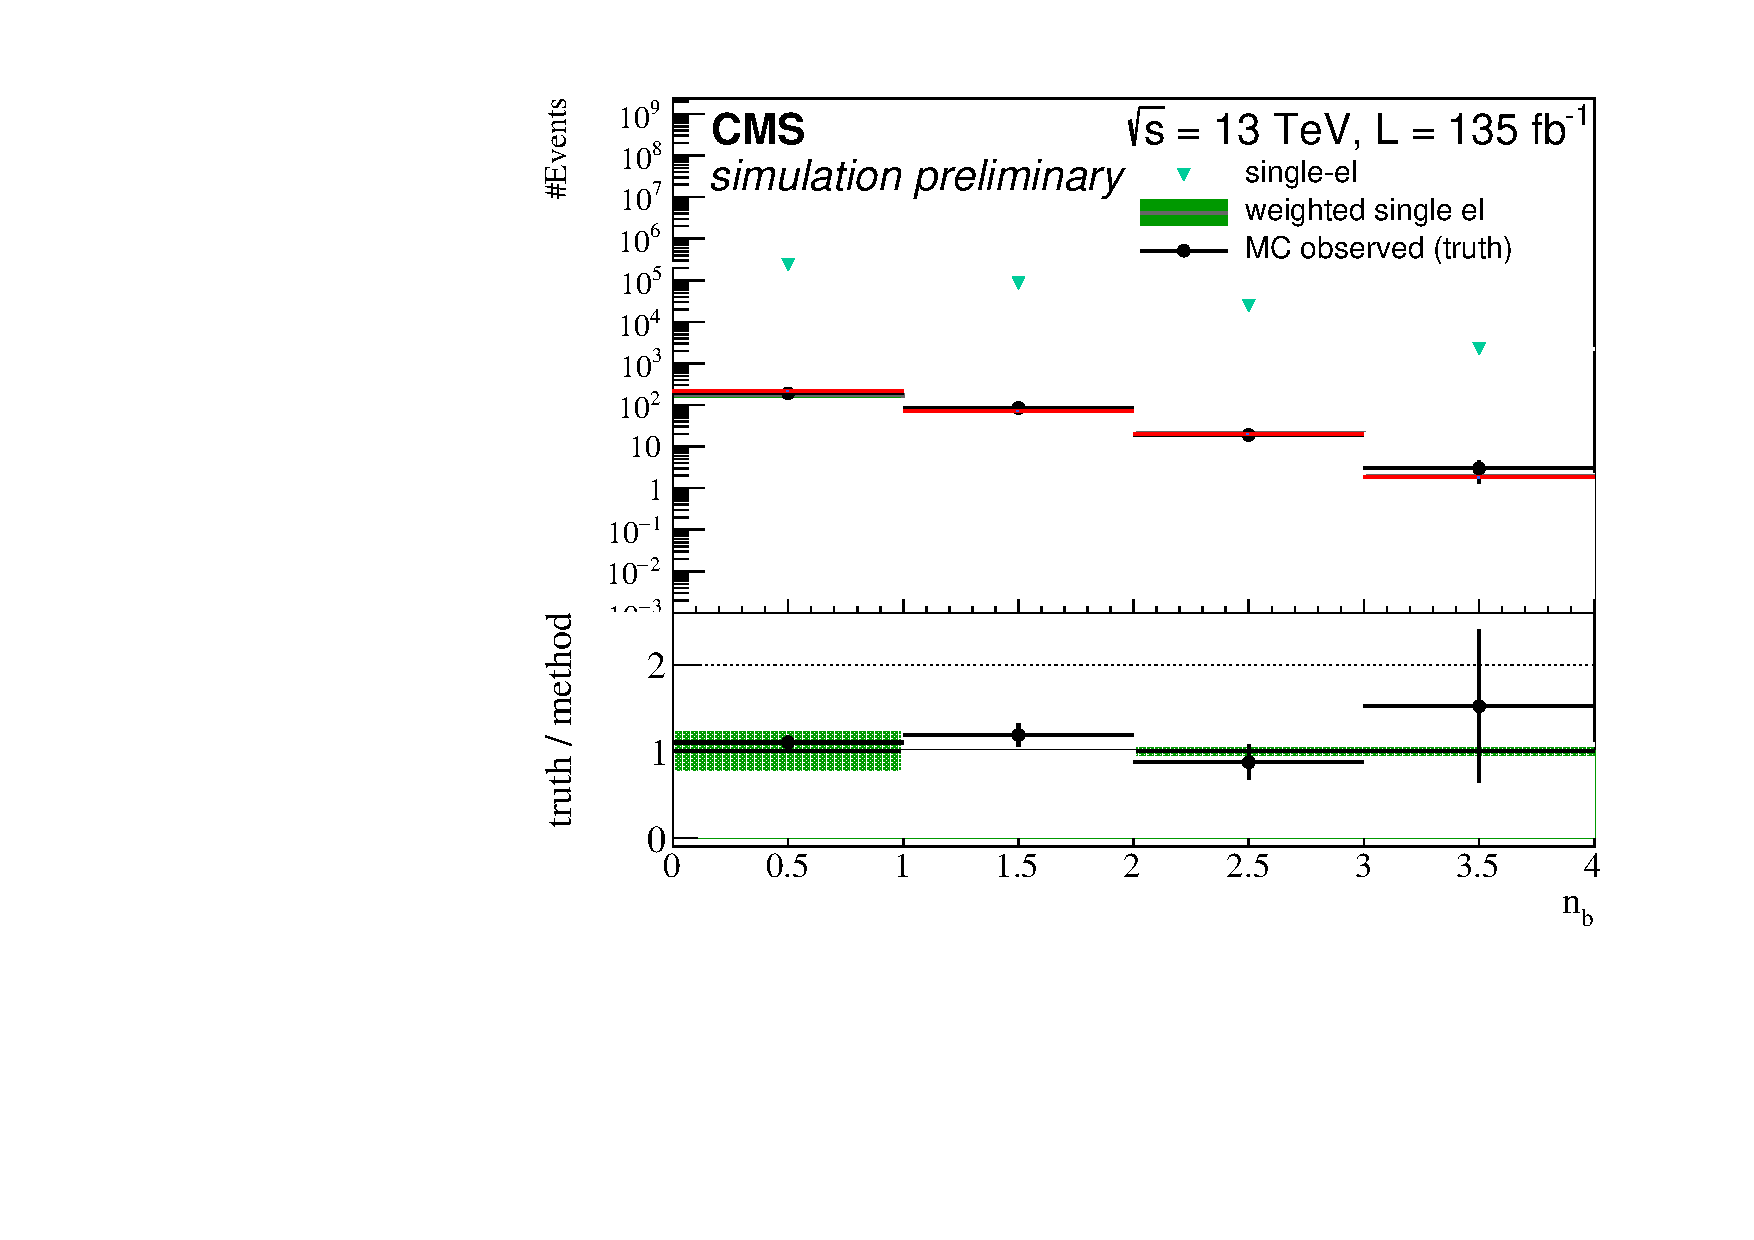
\includegraphics[width=0.8\linewidth]{pdfs/38-ElBaselineBTags.pdf}\\
\end{columns}
}

\frame{\frametitle{Muon background closure}
\begin{flushleft}
``n-1" post-baseline plots using W+jets and $t\bar{t}$-jets
\end{flushleft}
\vspace{-.1cm}
\centering
\begin{columns}
\column{.4\linewidth}
\centering
\scriptsize
MHT\\
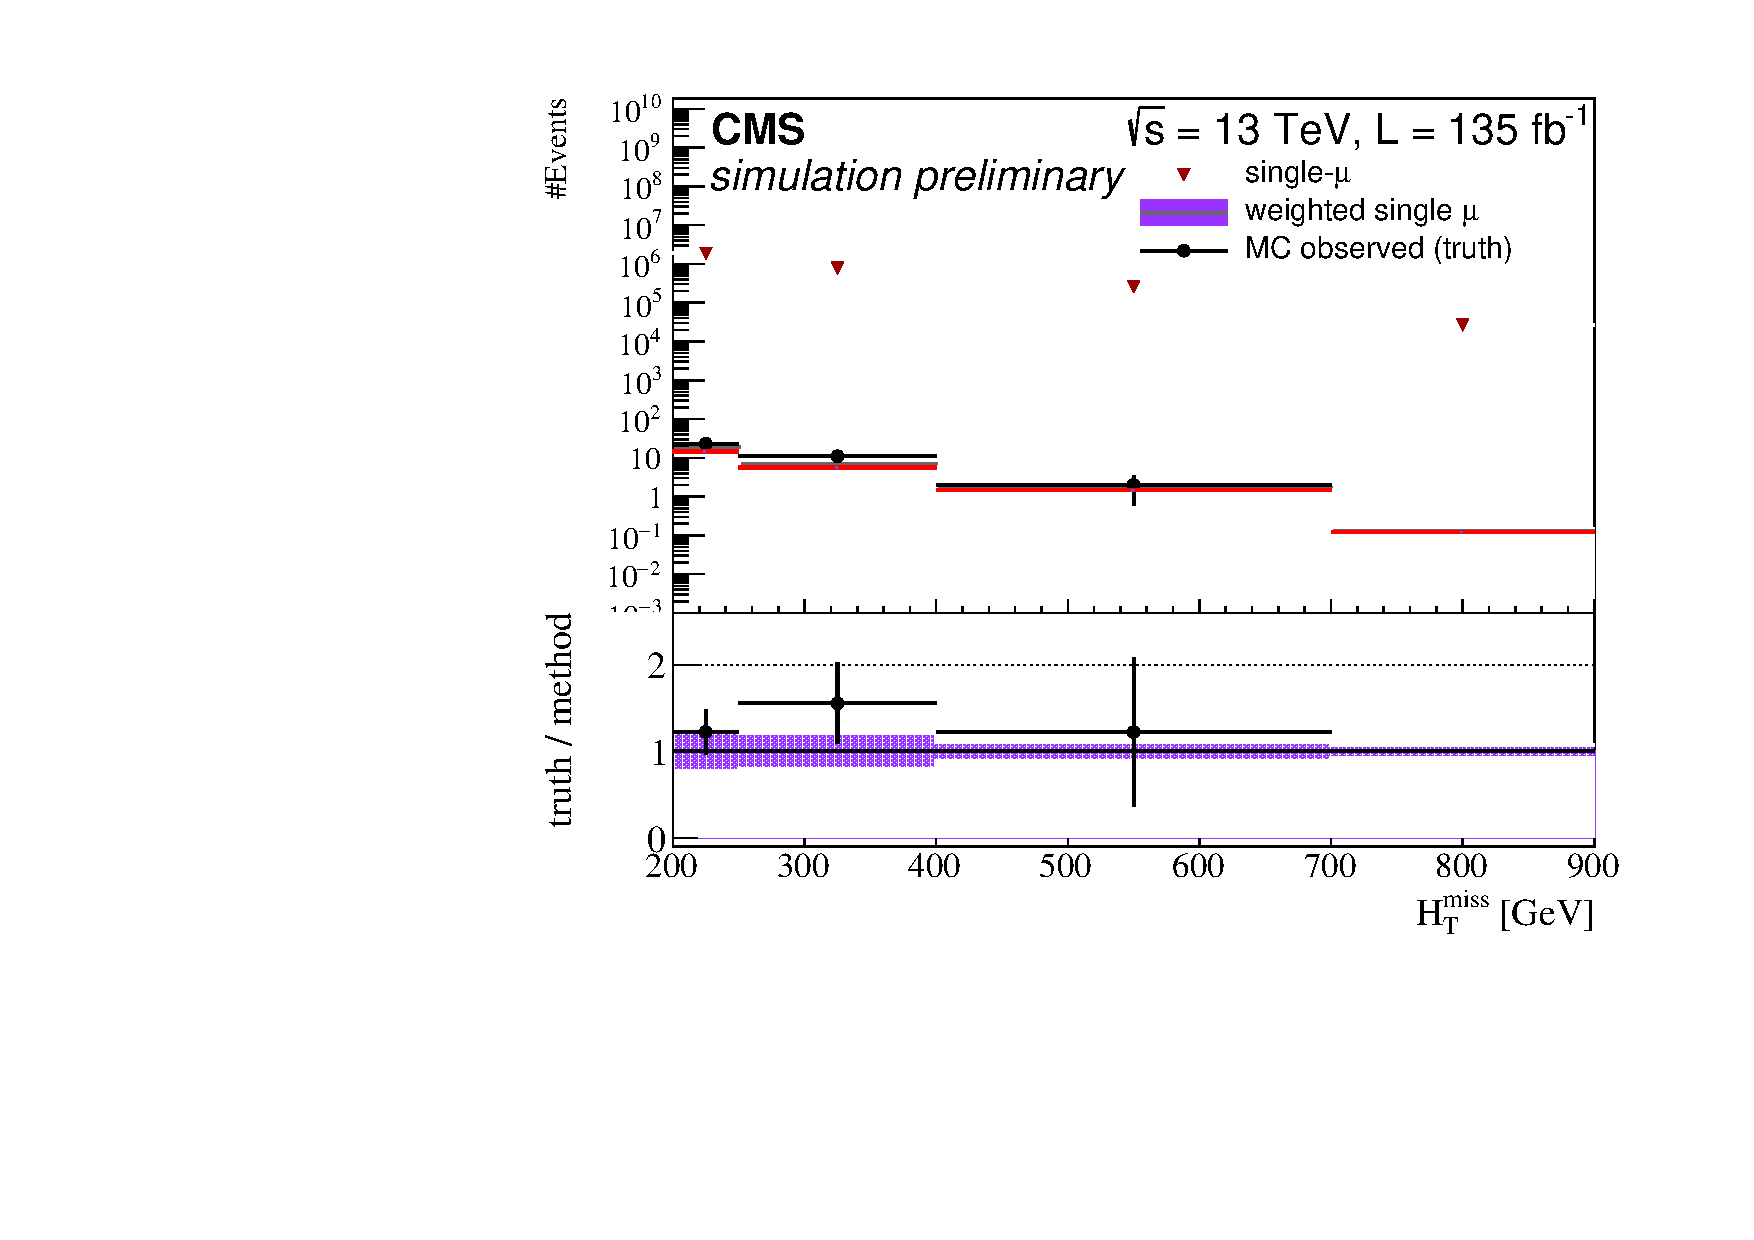
\includegraphics[width=0.8\linewidth]{pdfs/39-MuBaselineMht.pdf}\\
\scriptsize
n(jets)\\
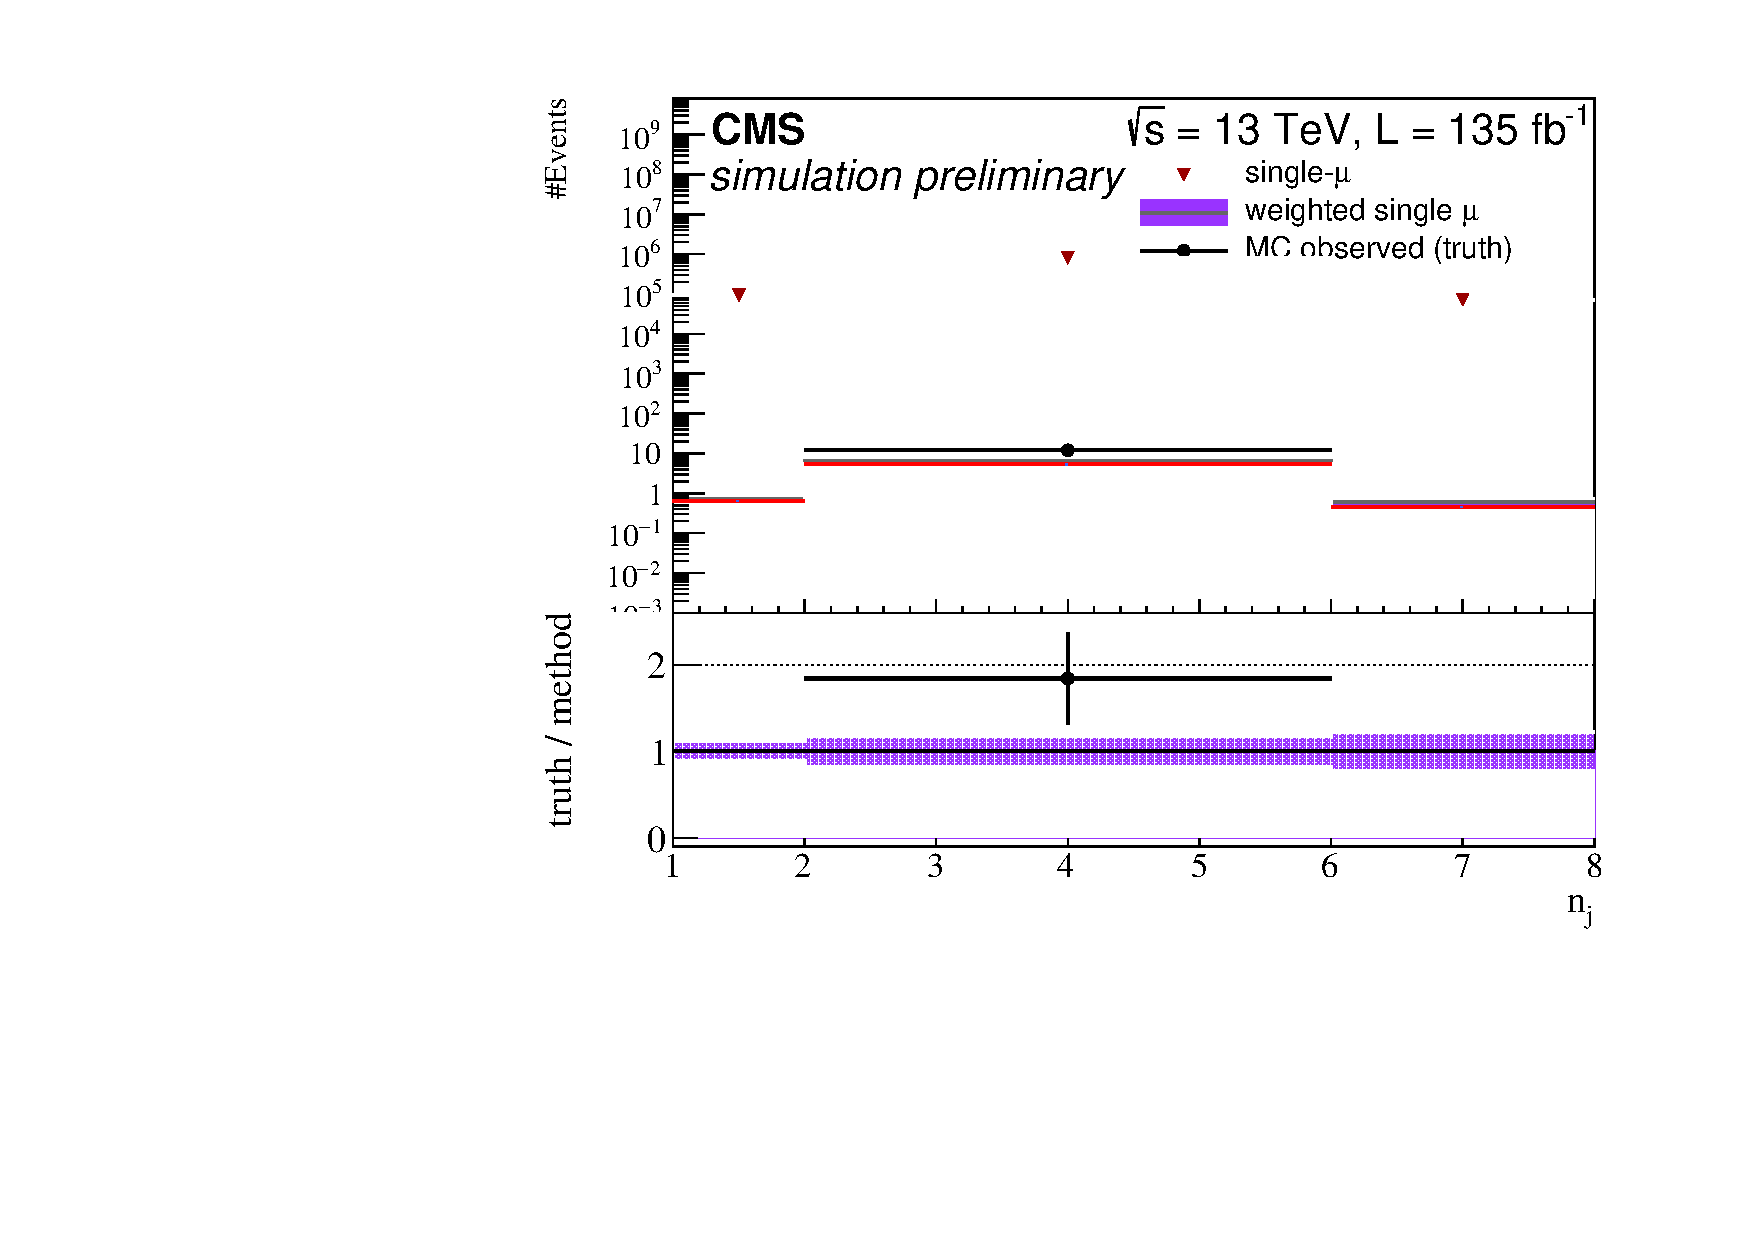
\includegraphics[width=0.8\linewidth]{pdfs/40-MuBaselineNJets.pdf}
\column{.4\linewidth}
\centering
\scriptsize
min($\Delta\phi$(jets, MHT))\\
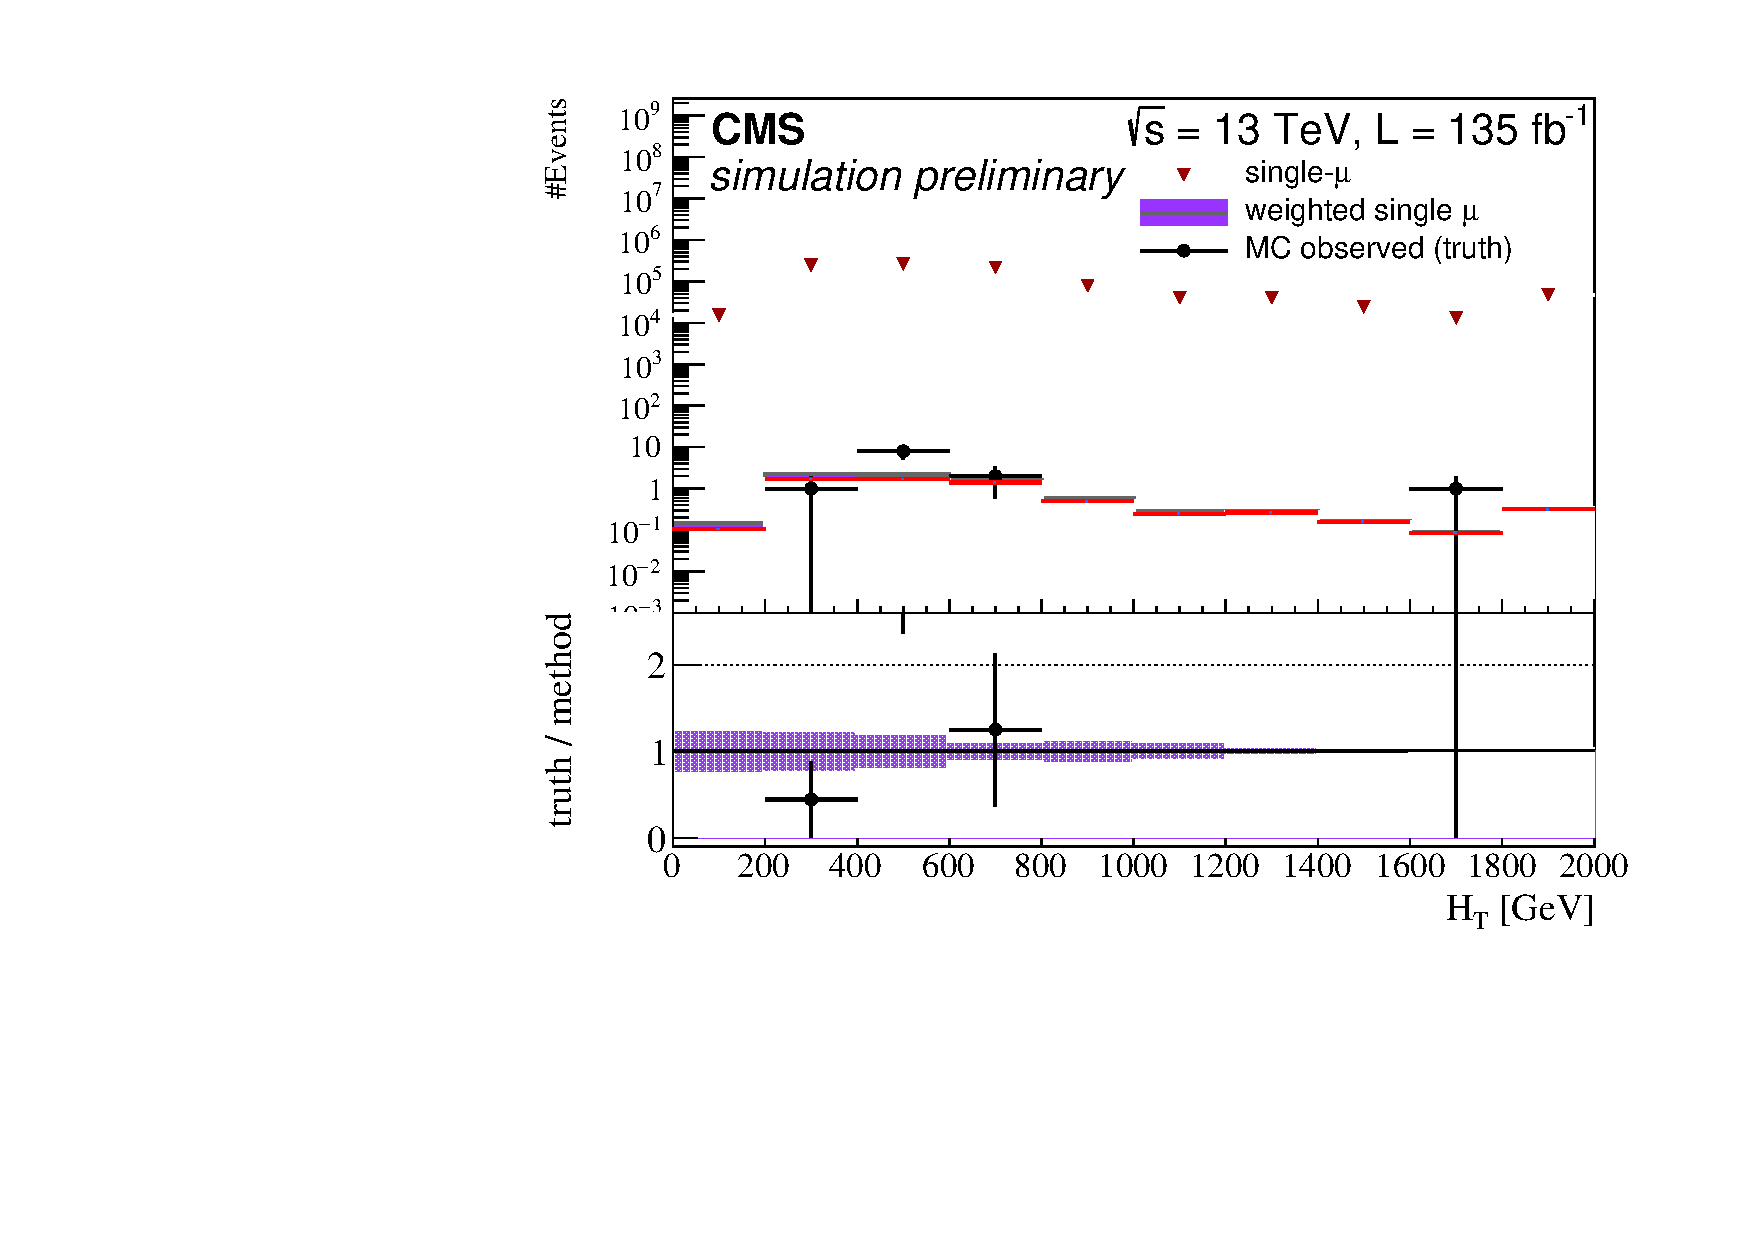
\includegraphics[width=0.8\linewidth]{pdfs/41-MuBaselineHt.pdf}\\
\scriptsize
n(b-tags)\\
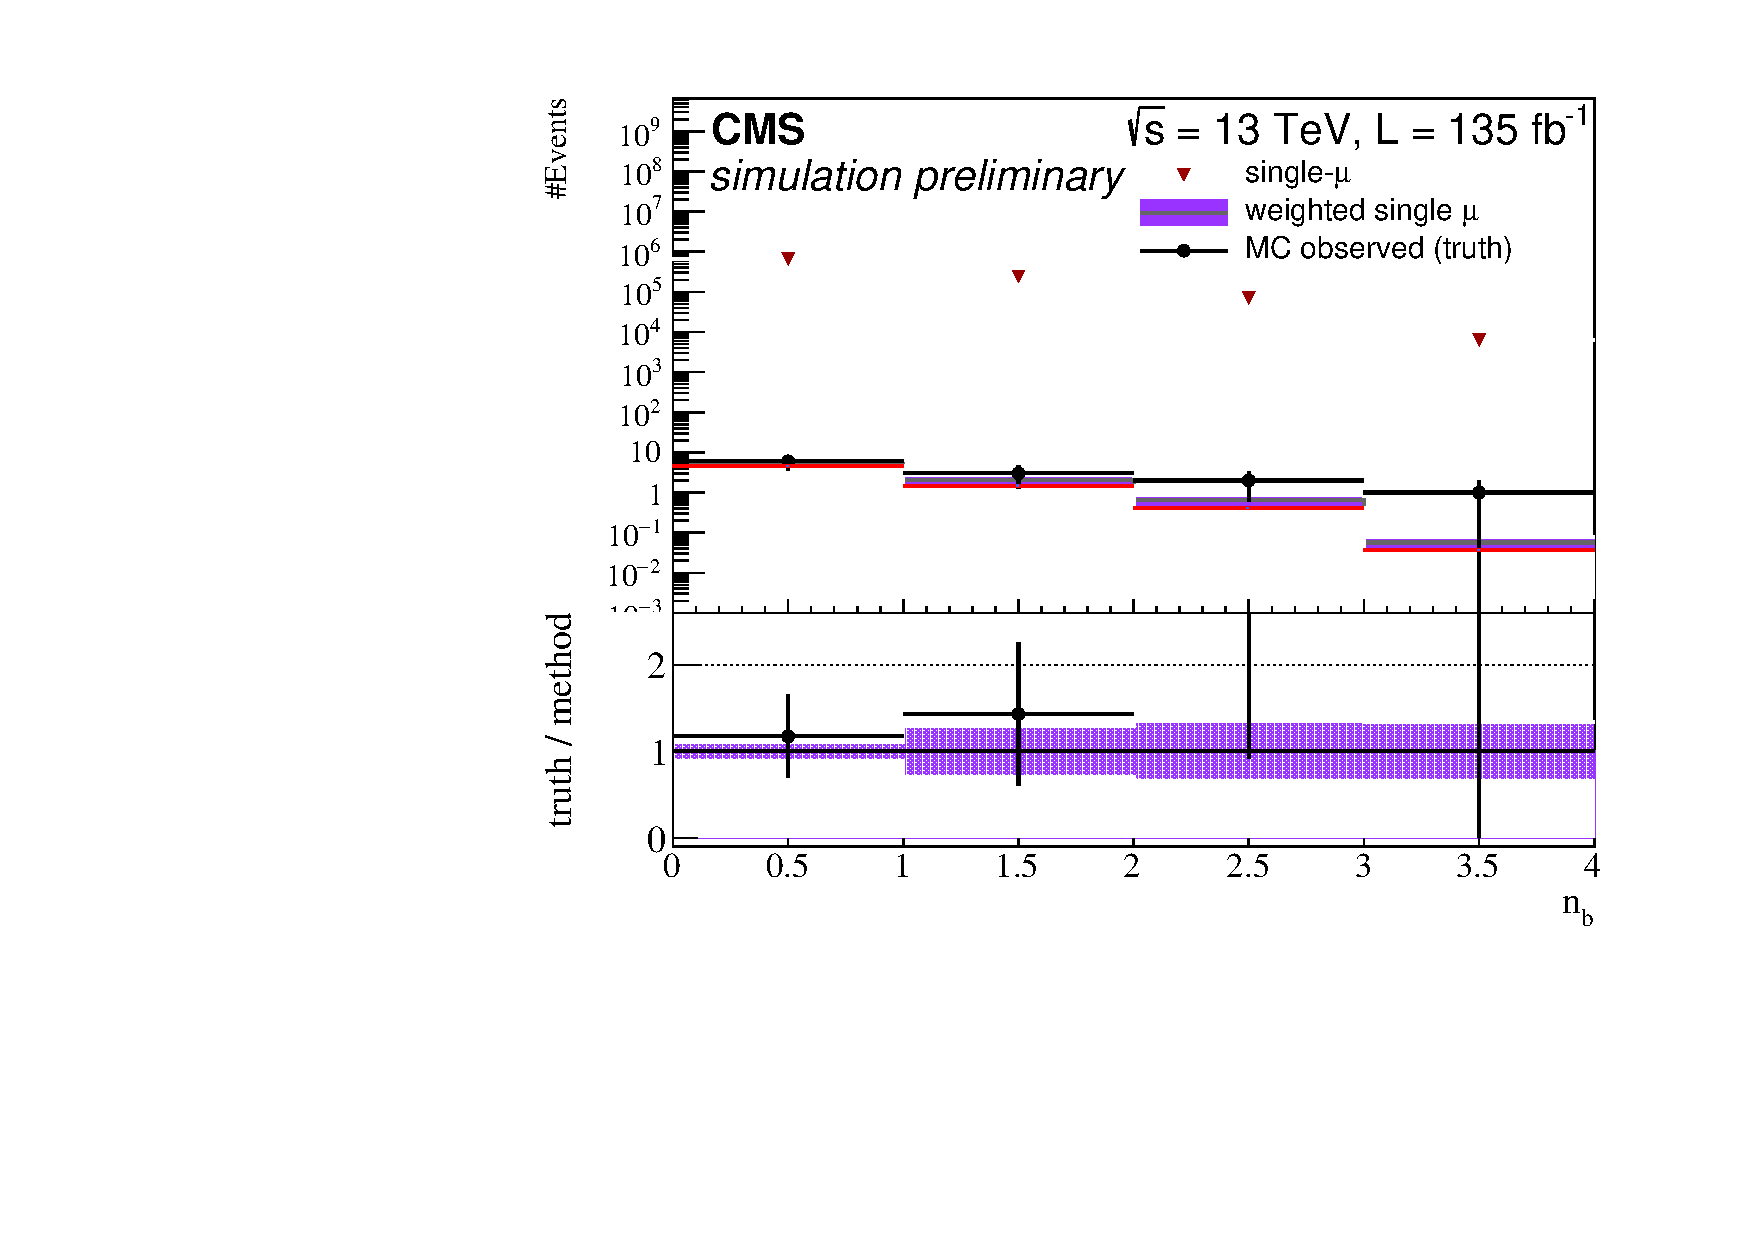
\includegraphics[width=0.8\linewidth]{pdfs/42-MuBaselineBTags.pdf}\\
\end{columns}
}


\frame{\frametitle{Prompt background: smearing dependence of $\kappa$}
\begin{columns}
\centering
\column{.4\linewidth}
\scriptsize
\begin{itemize}
\item Derive $\kappa$ factors smearing quality probes 
\item Derive $\kappa$ factors not smearing quality probes 
\item Make prediction with each version
\item Impact is not large since only the tails of the invariant mass are changed
\end{itemize}
\centering
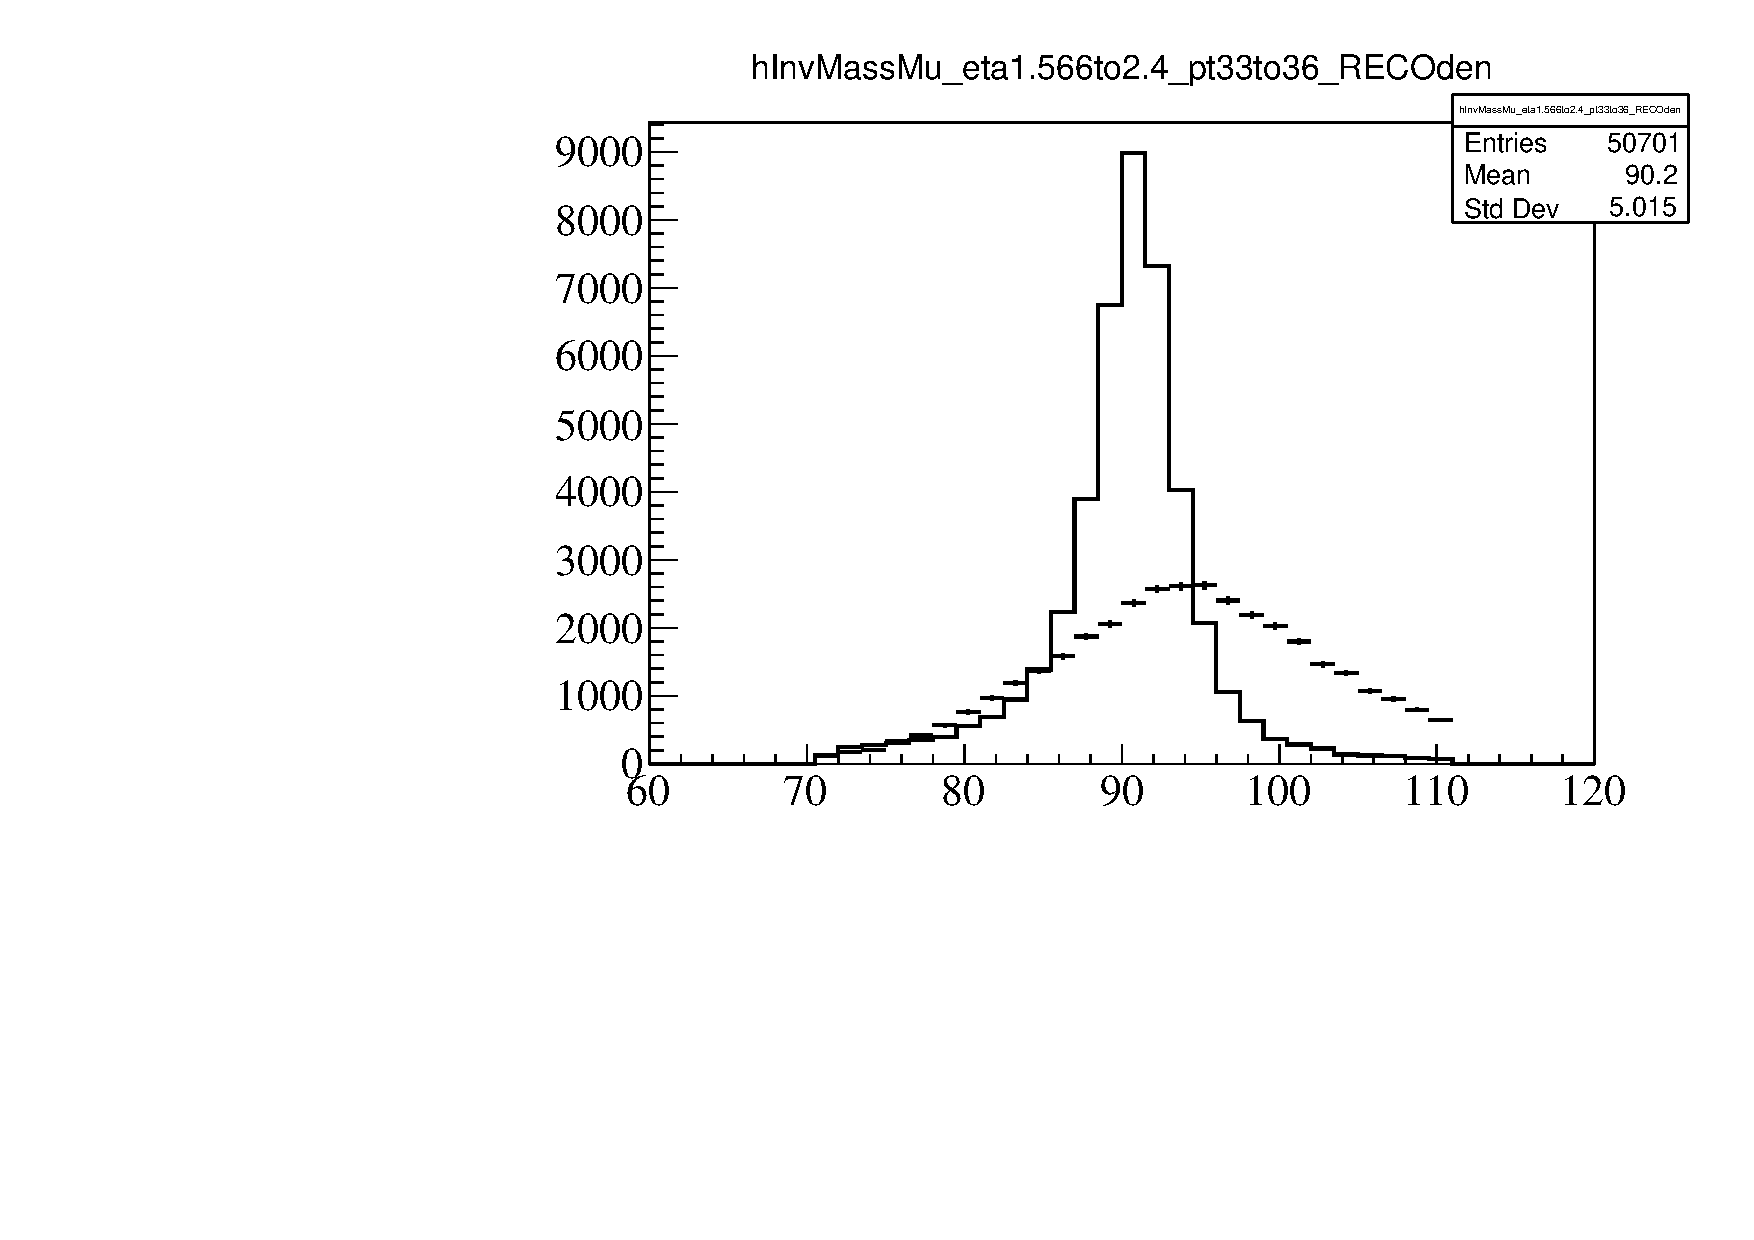
\includegraphics[width=0.9\linewidth]{pdfs/44-SmearedNonSmeared.pdf}
\column{.6\linewidth}
\centering
\scriptsize
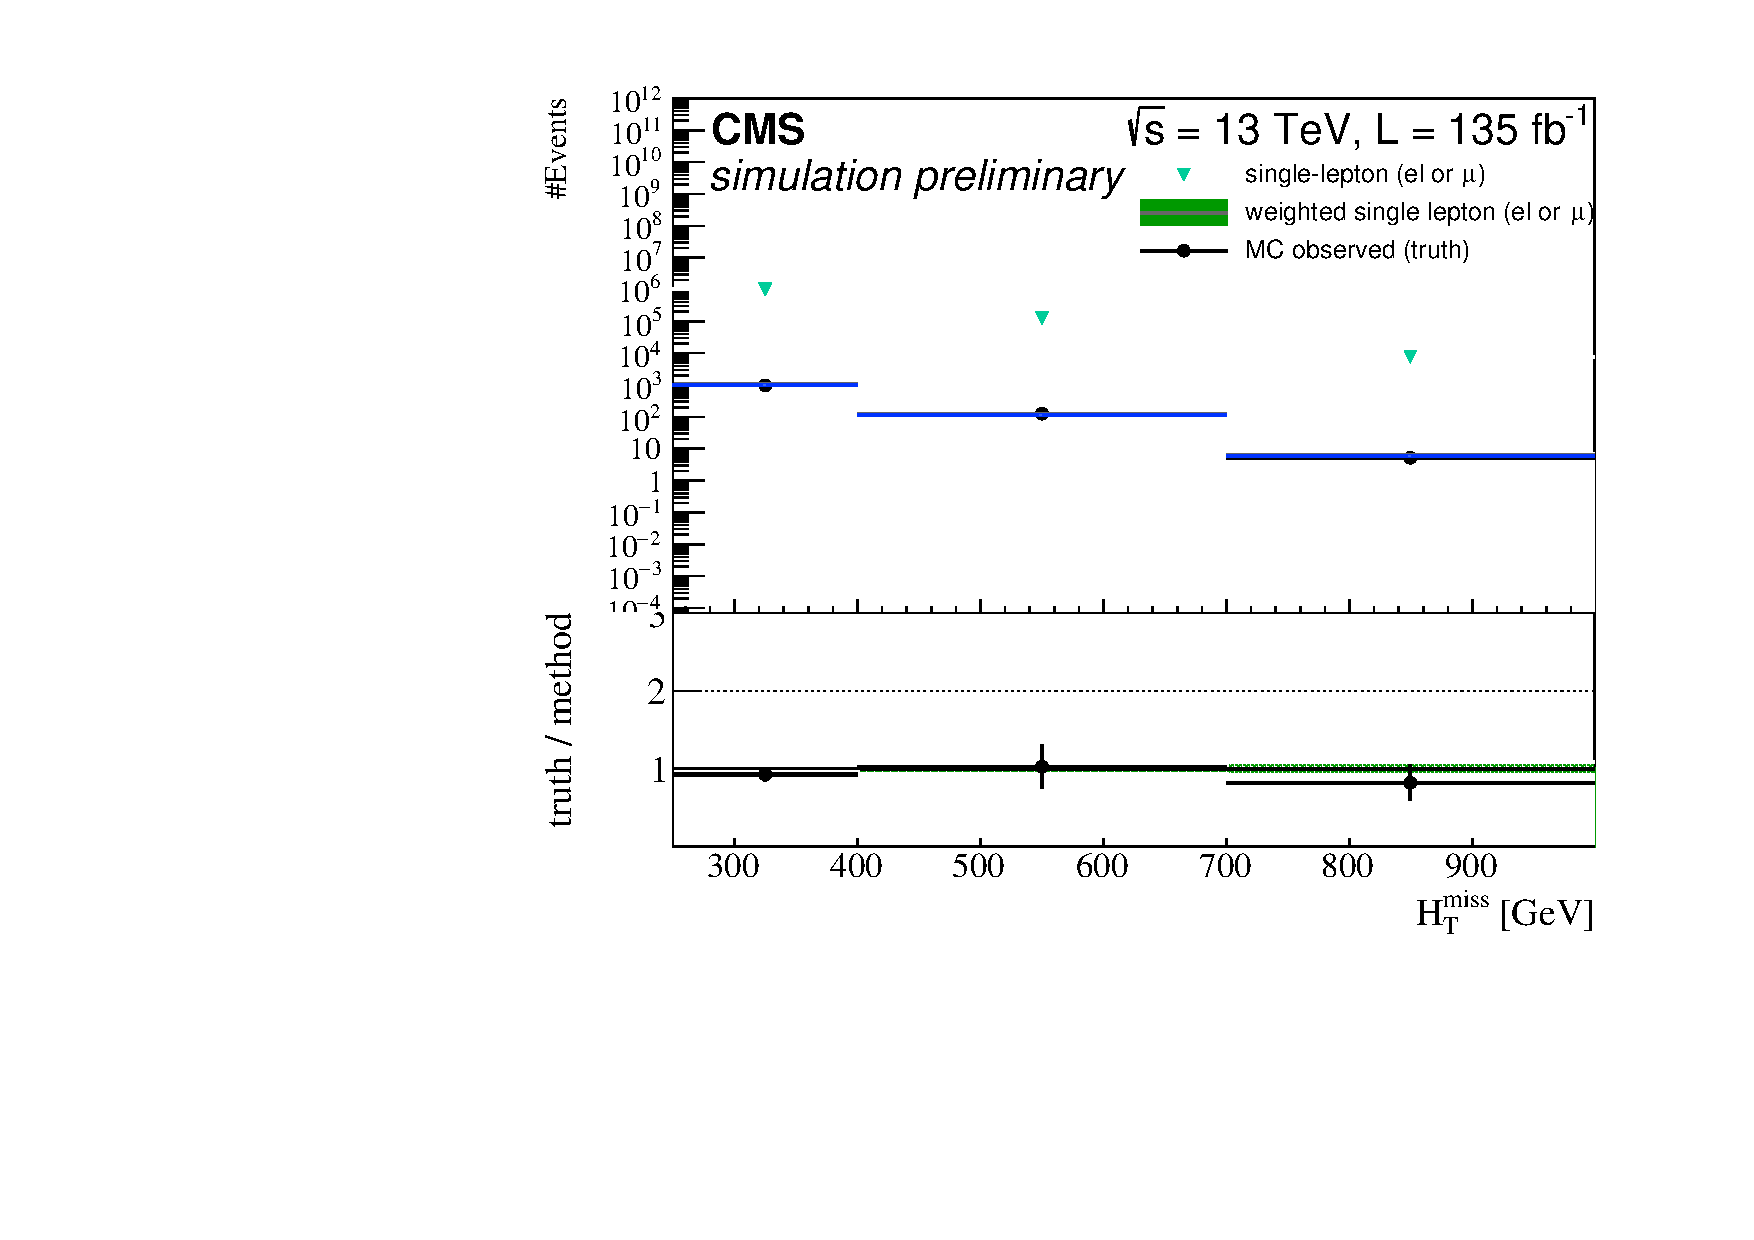
\includegraphics[width=0.5\linewidth]{pdfs/45-ElBaselineMht.pdf}
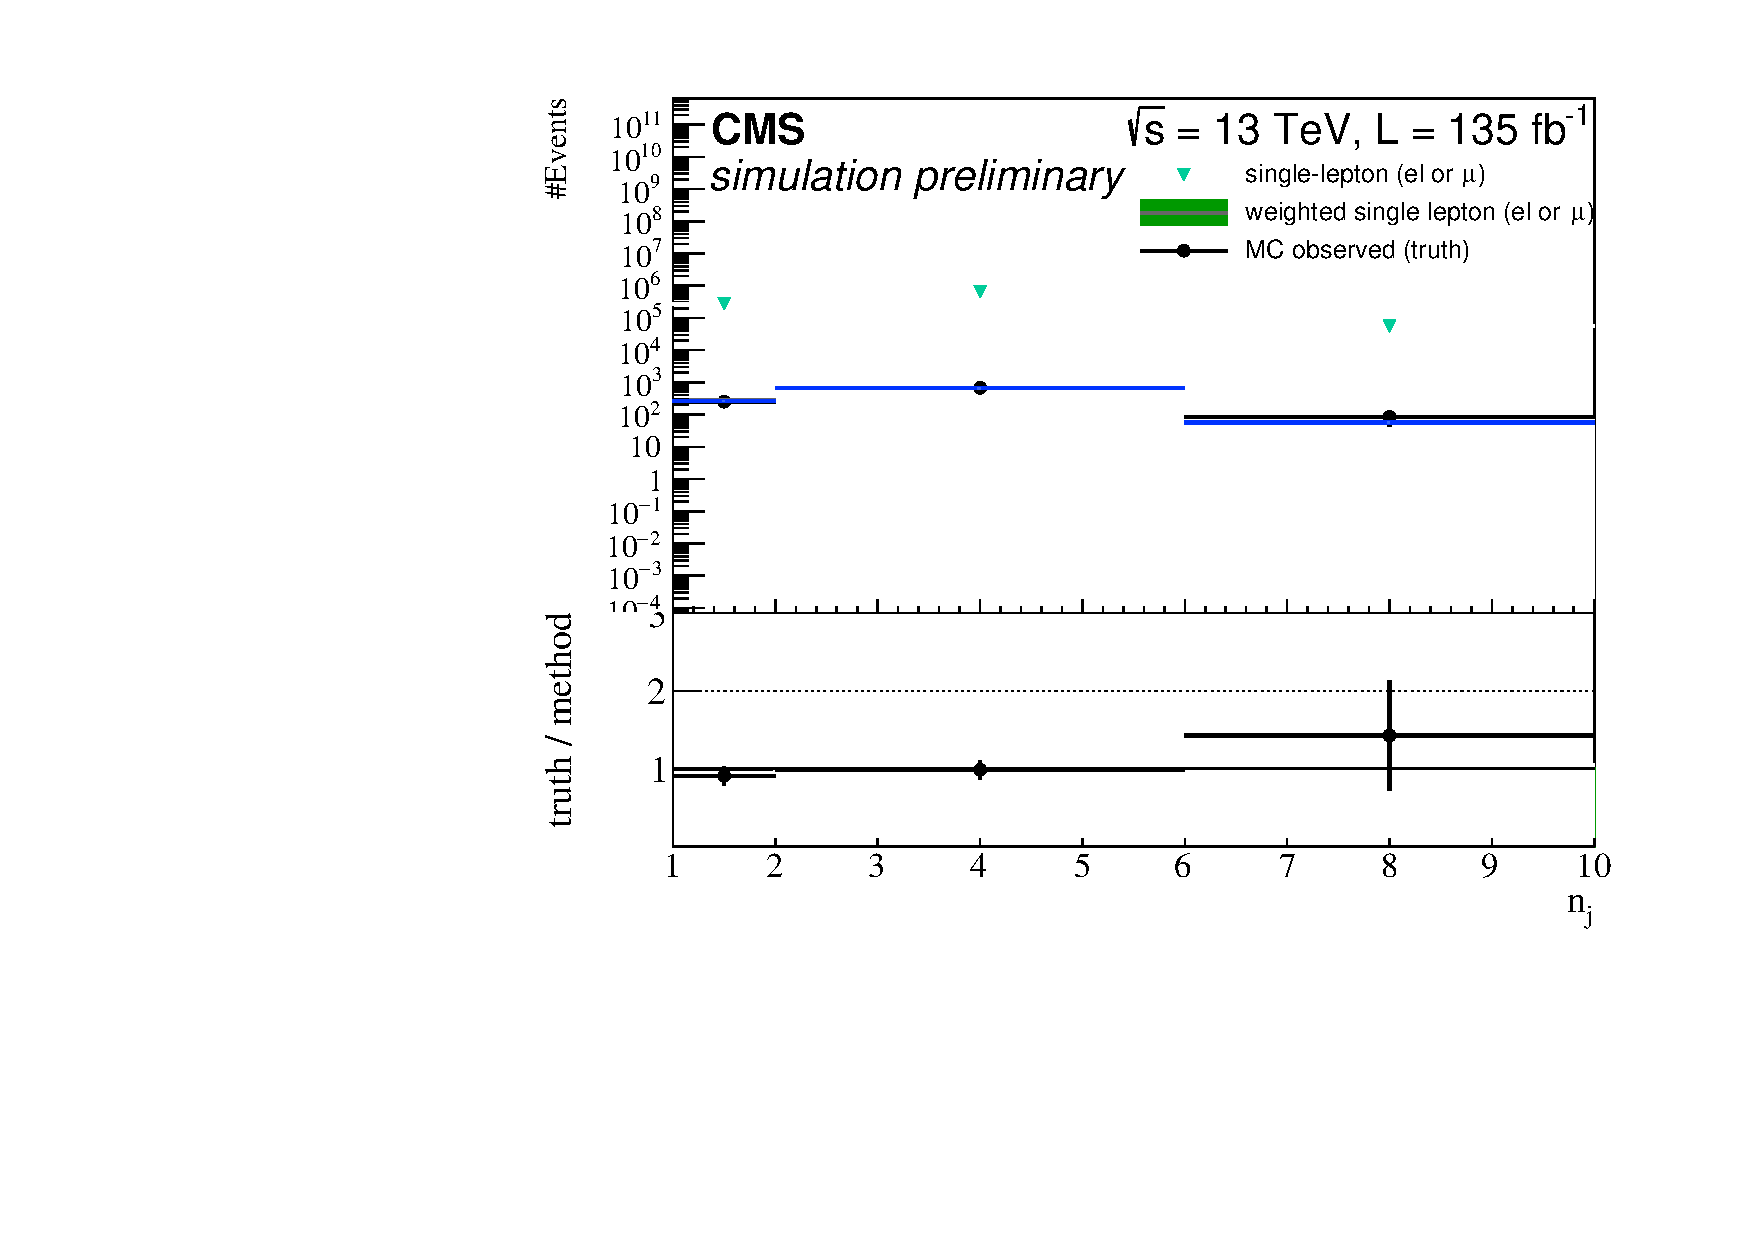
\includegraphics[width=0.5\linewidth]{pdfs/46-ElBaselineNJets.pdf}\\
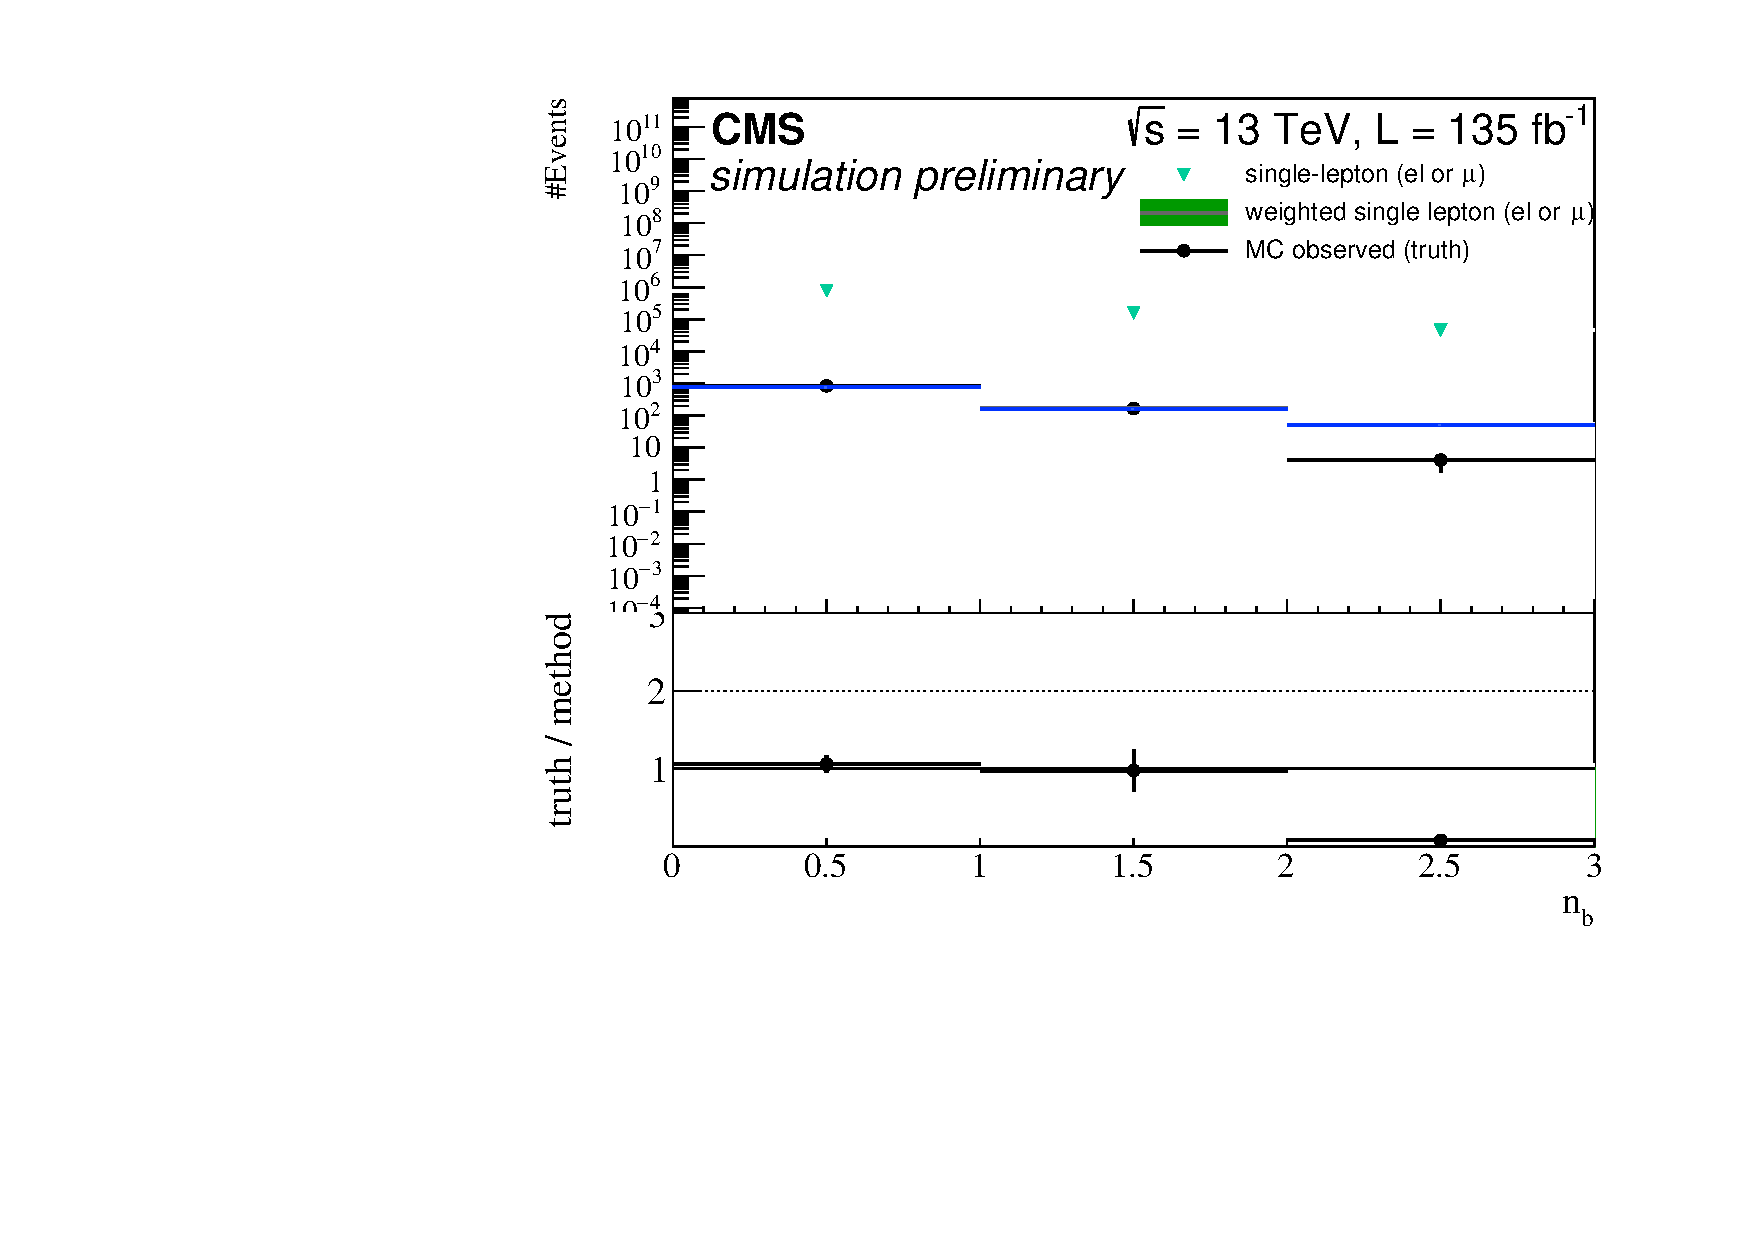
\includegraphics[width=0.5\linewidth]{pdfs/47-ElBaselineBTags.pdf}
\includegraphics[width=0.5\linewidth]{pdfs/48-ElBaselineNTags.pdf}
\end{columns}
}

\frame{\frametitle{}
\vspace{-.16cm}
\centering
\textbf{responses (pixel+strips) - barrel}
\includegraphics[width=.2\linewidth]{pdfs/49-hsmearFillOuthtrkresp0-1p4442-20-30El_PixAndStrips.pdf}
\includegraphics[width=.2\linewidth]{pdfs/50-hsmearFillOuthtrkresp0-1p4442-30-40El_PixAndStrips.pdf}
\includegraphics[width=.2\linewidth]{pdfs/51-hsmearFillOuthtrkresp0-1p4442-40-50El_PixAndStrips.pdf}
\includegraphics[width=.2\linewidth]{pdfs/52-hsmearFillOuthtrkresp0-1p4442-50-70El_PixAndStrips.pdf}
\includegraphics[width=.2\linewidth]{pdfs/53-hsmearFillOuthtrkresp0-1p4442-70-90El_PixAndStrips.pdf}\\
\includegraphics[width=.2\linewidth]{pdfs/54-hsmearFillOuthtrkresp0-1p4442-90-120El_PixAndStrips.pdf}
\includegraphics[width=.2\linewidth]{pdfs/55-hsmearFillOuthtrkresp0-1p4442-120-200El_PixAndStrips.pdf}
\includegraphics[width=.2\linewidth]{pdfs/56-hsmearFillOuthtrkresp0-1p4442-200-300El_PixAndStrips.pdf}
\includegraphics[width=.2\linewidth]{pdfs/57-hsmearFillOuthtrkresp0-1p4442-300-310El_PixAndStrips.pdf}\\
\textbf{responses (pixel-only) - barrel}
\includegraphics[width=.2\linewidth]{pdfs/58-hsmearFillOuthtrkresp0-1p4442-20-30El_PixOnly.pdf}
\includegraphics[width=.2\linewidth]{pdfs/59-hsmearFillOuthtrkresp0-1p4442-30-40El_PixOnly.pdf}
\includegraphics[width=.2\linewidth]{pdfs/60-hsmearFillOuthtrkresp0-1p4442-40-50El_PixOnly.pdf}
\includegraphics[width=.2\linewidth]{pdfs/61-hsmearFillOuthtrkresp0-1p4442-50-70El_PixOnly.pdf}
\includegraphics[width=.2\linewidth]{pdfs/62-hsmearFillOuthtrkresp0-1p4442-70-90El_PixOnly.pdf}\\
\includegraphics[width=.2\linewidth]{pdfs/63-hsmearFillOuthtrkresp0-1p4442-90-120El_PixOnly.pdf}
\includegraphics[width=.2\linewidth]{pdfs/64-hsmearFillOuthtrkresp0-1p4442-120-200El_PixOnly.pdf}
\includegraphics[width=.2\linewidth]{pdfs/65-hsmearFillOuthtrkresp0-1p4442-200-300El_PixOnly.pdf}
\includegraphics[width=.2\linewidth]{pdfs/66-hsmearFillOuthtrkresp0-1p4442-300-310El_PixOnly.pdf}
}



\frame{\frametitle{Prompt background: PU dependence of $\kappa$ }
\centering
\begin{columns}
\column{.4\linewidth}
\scriptsize
\begin{itemize}
\item merge all $p_{T}$ bins within a category of $\eta$, short/long, and electron/muon
\item compute $\kappa$ in data and MC in three bins of n(vtx)
\item scale ratio to the first bin value, modulo a presentation factor: $10^n$
\item no dominant trend for data or MC
\end{itemize}
\centering\column{.6\linewidth}
\centering
\scriptsize
\includegraphics[width=1.0\linewidth]{pdfs/67-KappaVsPileup.pdf}
\end{columns}
}


\frame{\frametitle{Systematics}
\begin{itemize}
\scriptsize
\item uncertainty in background predictions:
\begin{itemize}
\scriptsize
\item non-closure uncertainty
\item control region statistics (very small)
\item any additional systematic based on control region validation
\end{itemize}
\item signal systematics:
\begin{itemize}
\scriptsize
\item standard systematics 
\begin{itemize}
\scriptsize
\item JEC, JER
\item Pile-up
\item b-tagging and lepton scale factors
\item ISR systematic
\item FastSim MET correction
\item MC stats
\end{itemize}
\item disappearing electron scale factors
\end{itemize}
\end{itemize}
}


\backupend

\end{document}


